\documentclass[12pt,oneside]{report}
\usepackage[utf8]{inputenc}
\usepackage[T1]{fontenc}
\usepackage[english]{babel}
\usepackage{titlepic}
\usepackage{graphicx}
\usepackage[11pt]{moresize}
\usepackage{eso-pic}
\usepackage[export]{adjustbox}
\usepackage{fancyhdr}
\usepackage{vmargin}
\usepackage{titlesec}
\usepackage{textpos}
\usepackage{minted}
\usepackage{float}
\usepackage[breaklinks=true,hidelinks]{hyperref}
\usemintedstyle{manni}

\renewcommand{\thesection}{\arabic{section}}
\renewcommand{\thefigure}{\arabic{chapter}.\arabic{section}.\arabic{figure}}

\newcommand{\HRule}{\rule{\linewidth}{0.5mm}}

%%%% Footer and Header %%%%%%%%%%%%%%

\pagestyle{fancy}
\fancyhf{}
\fancyfoot[C]{\footnotesize{\rightmark}}
\fancyfoot[R]{Page -- \thepage}
\renewcommand{\footrulewidth}{0.5pt}
\renewcommand{\headrulewidth}{0pt}


% Redefine the plain page style
\fancypagestyle{plain}{
\fancyhf{}
\fancyfoot[C]{\footnotesize{\rightmark}}
\fancyfoot[R]{Page -- \thepage}
\renewcommand{\footrulewidth}{0.5pt}
\renewcommand{\headrulewidth}{0pt}
}

\begin{document}
%----------------------------------------------------------------------------------------
%	MARGINS
%----------------------------------------------------------------------------------------
\setmarginsrb{ 1.2in}   % left margin
             { 0.6in}   % top margin
             { 1.2in}   % right margin
             { 0.8in}   % bottom margin
             {  20pt}   % head height
             {0.25in}   % head sep
             { 9pt}     % foot height
             { 0.75in}  % foot sep

%%%%%%% Title Page %%%%%%%%%%%%%%%%%%%

%---title format---
%%%%%%%%%%%%%%%%%%%%%%%%%%%%%%%%%%%

\titleformat{\chapter}[display]
{\normalfont\Large\bfseries}
{} % label
{0.5ex} % sep
{
	\rule{\textwidth}{1pt}
	\vspace{1ex}
	\centering
} % before-code
[
\vspace{-0.5ex}%
\rule{\textwidth}{0.3pt}
] % after-code

\titlespacing*{\chapter} {0pt}{0mm}{2mm}   
%%%%%%%%%%%%%%%%%%%%%%%%%%%%%%%%%%%%

	\begin{titlepage}
		\begin{center}
			\vspace*{\fill}
			
 			\begin{figure}[h]
       	 		
\includegraphics[width=4cm, center]{Figures/LogoEcam.png}	
       	 	\end{figure}
 			\vspace{\baselineskip}
 			
       		\HUGE{Kitbox Sales Interface}
       		\vspace{0.5cm}


       		\normalsize{Juin 2018} 
			
       		\vspace*{\fill}
       		
       		\large{DENIS Maxime 15089 \\
                DUCOULOMBIER Théo 16067\\
                SCARITO Michaël 16117\\
                SMITS Victor 16107\\
                SNYERS Harold 16243}
            \vspace{\baselineskip}
            
            \large{Ecole centrale des arts et métiers}
            \vspace{\baselineskip}
            
       		\small{BAC 3 Génie Électrique}
       		\vspace{\baselineskip}
       		
       		\normalsize{Année académique 2018-2019}
   		\end{center}
	\end{titlepage}

%%%%% table of content %%%%%%
\tableofcontents

\newpage
%%%%% begin report %%%%%%
\chapter{Kitbox Sales Interface}
\vspace{\baselineskip}
\vspace{\baselineskip}

\section{Introduction}
    \paragraph{}
    As part of the "Génie Logiciel" course, we were asked to create an application for the furniture manufacturer "Kitbox". The company needed an interface so that customers could order their furniture more efficiently and thus reduce the workload of the storekeepers. In this report, we will start by carrying out an analysis of the needs of the company. We will then review the various diagrams that have allowed us to arrive at an appropriate solution. Finally, we will focus on the different pages of the application. Those allow the user to create a custom-made or standard sized cabinet, to get information about the company or to consult his cart.

\newpage
\section{Needs Analysis}
    \paragraph{} Prior to rush on the solution, we needed to analyse and understand the real problem. Here we have a list of all the requirements and additional options.
    \vspace{\baselineskip}
    
    The application must be capable of:
    \begin{itemize}
        \item Creating a cabinet with standard dimensions or not.
        \item Updating the database reservation section with the current order.
        \item Checking if all the parts are available in the stock.
        \item Telling the customer he has to pay in advance if some pieces are missing.
        \item Calculating the price for one cabinet and for the final cart.
        \item Gather all the information about an element of a cabinet (Stock reference, price, remaining quantity in stock).
        \item If a cabinet is erased, the database must update the reservation section.
        \item Asking for the customer’s email when finishing the order.
        \item Displaying only the dimension and colour corresponding with the current combination.
    \end{itemize}
    \vspace{\baselineskip}
    
    The application could be able to :
    \begin{itemize}
        \item Display the cabinet while the customer is working on it.
        \item Having a page displaying information about the company.
        \item Display a progress bar when adding a cabinet to the cart. 
        \item Display images on the homepage.
    \end{itemize}
    \vspace{\baselineskip}
    
    The user must be capable of :
    \begin{itemize}
        \item Selecting the colour of his choice for each floor of a cabinet.
        \item Adding a door if he wants to.
        \item Going to the creation page in an user friendly way.
        \item Knowing the final dimensions of his cabinet without calculating.
        \item Creating a cabinet easily.
        \item Deleting a cabinet after creating it.
    \end{itemize}
    \vspace{\baselineskip}
    
    \newpage
    The user could be able to : 
    \begin{itemize}
        \item Sign in for a newsletter.
        \item Interact with the cabinet which displayed in the creation page.
    \end{itemize}
    \vspace{\baselineskip}

    The storekeeper must be capable of :
    \begin{itemize}
        \item Updating the order status.
        \item Finding an order by its reference.
        \item Getting information about the remaining stock.
        \item Closing order when the customer has pay.
        \item Adding parts in the stock.
        \item Modifying the price of parts.
        \item Gather the part's list of an order.
        \item Seeing parts which need to order.
        \item Registering customer information.
        \item Creating profile for customers.
    \end{itemize}
    \vspace{\baselineskip}

    There are still some technical requirements as the project must operate on \textit{Windows 8X86} or above, have an \textit{Access Database}, be up-gradable and responsive.

\newpage
\section{Diagrams}
    \subsection{Activity}
        \paragraph{}
        To understand this diagram, we need to begin on the black dot in the top centre (\textit{Figure \ref{activitydiagram}}). The customer asks for the catalogue before placing an order. Once he is decided to buy something, he has to confirm his order before completing it. Here begins the storekeeper’s interface. 
        
        \paragraph{}
        First things first, it is necessary to check if all the parts needed are in stock. If not, the storekeeper must order it and ask the customer to pay an advance. When all the parts are in stock, the storekeeper must provide an invoice, and the customer must pay the total amount, or the remaining sum if he had to wait for some parts.
        
        \paragraph{}
        When all of those steps have been completed, the storekeeper prints the parts’ list before gathering them all and closing the order. Finally, the customer may leave the store with his order to take it home. 
    \vspace{\baselineskip}
    \vspace{\baselineskip}
    
    \subsubsection{Activity standard dimension}
        \paragraph{}
        As there are two ways to create a cabinet, there are also two activity diagrams related to it. The first one deals with the creation based on standard dimension (\textit{Figure \ref{activitystandartdiagram}}). It is very simple, the user must choose one of the standard height, width and depth. If he wishes to, he can modify the visual aspect of the box or add a door before confirming his cabinet.
    \vspace{\baselineskip}
    \vspace{\baselineskip}
    
    \subsubsection{Activity cabinet creation}
        \paragraph{}
        The second way allows the user to fully customise his cabinet by adding boxes of the same width and depth on top of each other (\textit{Figure \ref{activitycabinetdiagram}}). As long as the cabinet does not exceed the maximum height or number of boxes, the user is allowed to add a box to the cabinet and customise it. By customising, we mean choosing the colour and adding a door. Once the cabinet is done and confirmed, the software must compute the right angle to take. If it is not a standard dimension, the size directly above is chosen, and the angle is cut to the desired size. The command can then be confirmed.
    \newpage
    
    \subsection{Use case}
        \paragraph{}
        The use case diagram (\textit{Figure \ref{usecasediagram}}) shows us the actors and the main actions to interact with the application. In our case, we have two main actors, the customer and the storekeeper. We decided, with our client, what the customer should be able to do. 
        
        \paragraph{}
        With the user interface, the customer should be able to consult the catalogue, order a cabinet or pay it. Consulting the catalogue means that he can look through the different parts from the database. Once he has decided to buy a cabinet, two choices are offered to the user, finalise the order or create a new one. When he has confirmed his order, he must pay for it. 
        
        \paragraph{}
        There are two possibilities. First, some of the needed parts are out of stock; the storekeeper must order it. An advance will be asked to the customer, and the rest will be paid once all the ordered parts are in stock. The second possibility is that all the parts are in stock. Therefore the customer must pay the total amount and can leave with his cabinet. The storekeeper can act as a customer and therefore, use all those actions as well.
        
        \paragraph{}
        We can link three main use cases to the storekeeper. The first one allows him to see the progress of the orders in the form of list. Once he has chosen an order in this list, he can get the part’s list to gather those. In this use case he can also search for an order based on the order number. To end this case he can finally close a pending order. For example, when the order leaves the warehouse.\\
        The second case offers him the possibility to fill the stock. It means that once he receives a restocking, the storekeeper has to update his stock. Finally, the third case gives him an overview on the current stock.
    
    \newpage
    \subsection{Class diagram}
        \paragraph{}
        The source code is based on a pattern composite (\textit{see Figure \ref{compositepattern}}), which allows us to create a cabinet which is composed of different elements described further. The cabinet is composed of objects which are described thanks to properties such as their price, stock reference, quantity, visual and physical description.
        \vspace{\baselineskip}
        
        \begin{figure*}[h!]
            \centering
			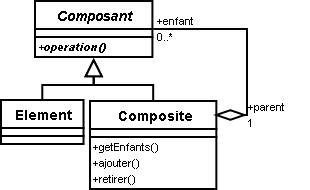
\includegraphics[width = 0.5\textwidth]{Figures/composite.png}
			\caption{Composite Design Pattern}
			\label{compositepattern}
		\end{figure*} 
			
        \paragraph{}
        Interfaces are there to gather all the parts of an element, for example, the IStorageBox interface assembles the empty box (without door) and the double door if needed. It assures the scalability of our application. Abstract classes set the shared methods of the object put together. Thanks to those classes, we avoid repetition in the code. This and the scalability are two main points of the object-oriented programming.
        
        \paragraph{}
        A cabinet is composed of boxes which make up one or more floor. The customer can choose to add doors if he wishes. Those boxes are made of several components reunited by the IComponent interface and GenericComponent.
        
        \paragraph{}
        The object named “Cart” (\textit{see Figure \ref{cartclass}}) enables us to link the customer’s purchase to his email address. This process leads to easier order recognition. All the elements in the cart are then added in a JSON string send to the interface to be displayed. We have chosen to use JSON for its ability to set and find values to a certain key. This structure simplifies our work in the interface and allows us to send a representation of the cart to the database. 
        \vspace{\baselineskip}
         
        \begin{figure*}[h!]
            \centering
			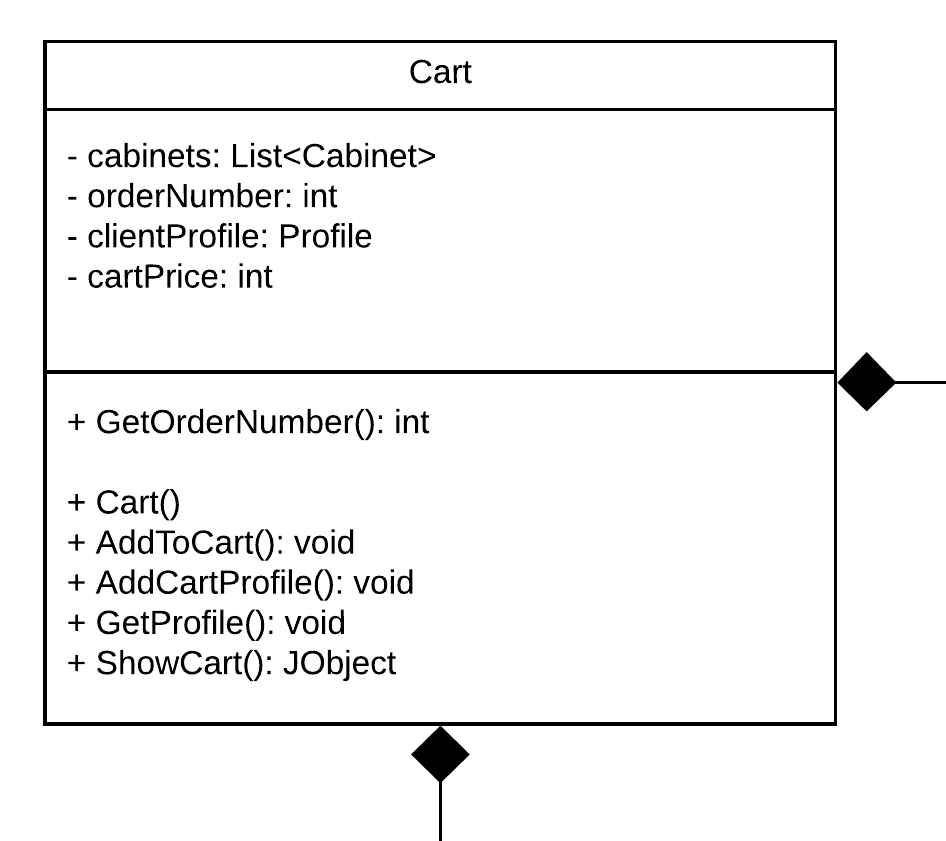
\includegraphics[width = 0.4\textwidth]{Figures/CartClass.png}
			\caption{Class Cart}
			\label{cartclass}
		\end{figure*} 
		
		\newpage
        \paragraph{}
        When a floor’s component is generated, four SQL requests are executed. The first one allows to retrieve the stock reference according to the characteristics. The second one updates the reservation column and the third one gets the price. Finally, the last one gets the remaining quantity in the stock.
        
        
        \paragraph{}
        Thanks to a dll package, we integrate the source code with the interface, therefor only a few commands are required: cart creation, cabinet creation, cabinet floor creation, adding the floor in the cabinet and adding cabinet in cart (\textit{see Figure \ref{cabinetclass}}). To create the “CabinetFloor”, those attributes are needed: length, depth, height, colour and door colour. The double door will only be automatically generated if the “DoorColor” attribute is set. You can find the complete diagram in the appendix \ref{classdiagram}.
        \vspace{\baselineskip}
        
        \begin{figure*}[h!]
            \centering
			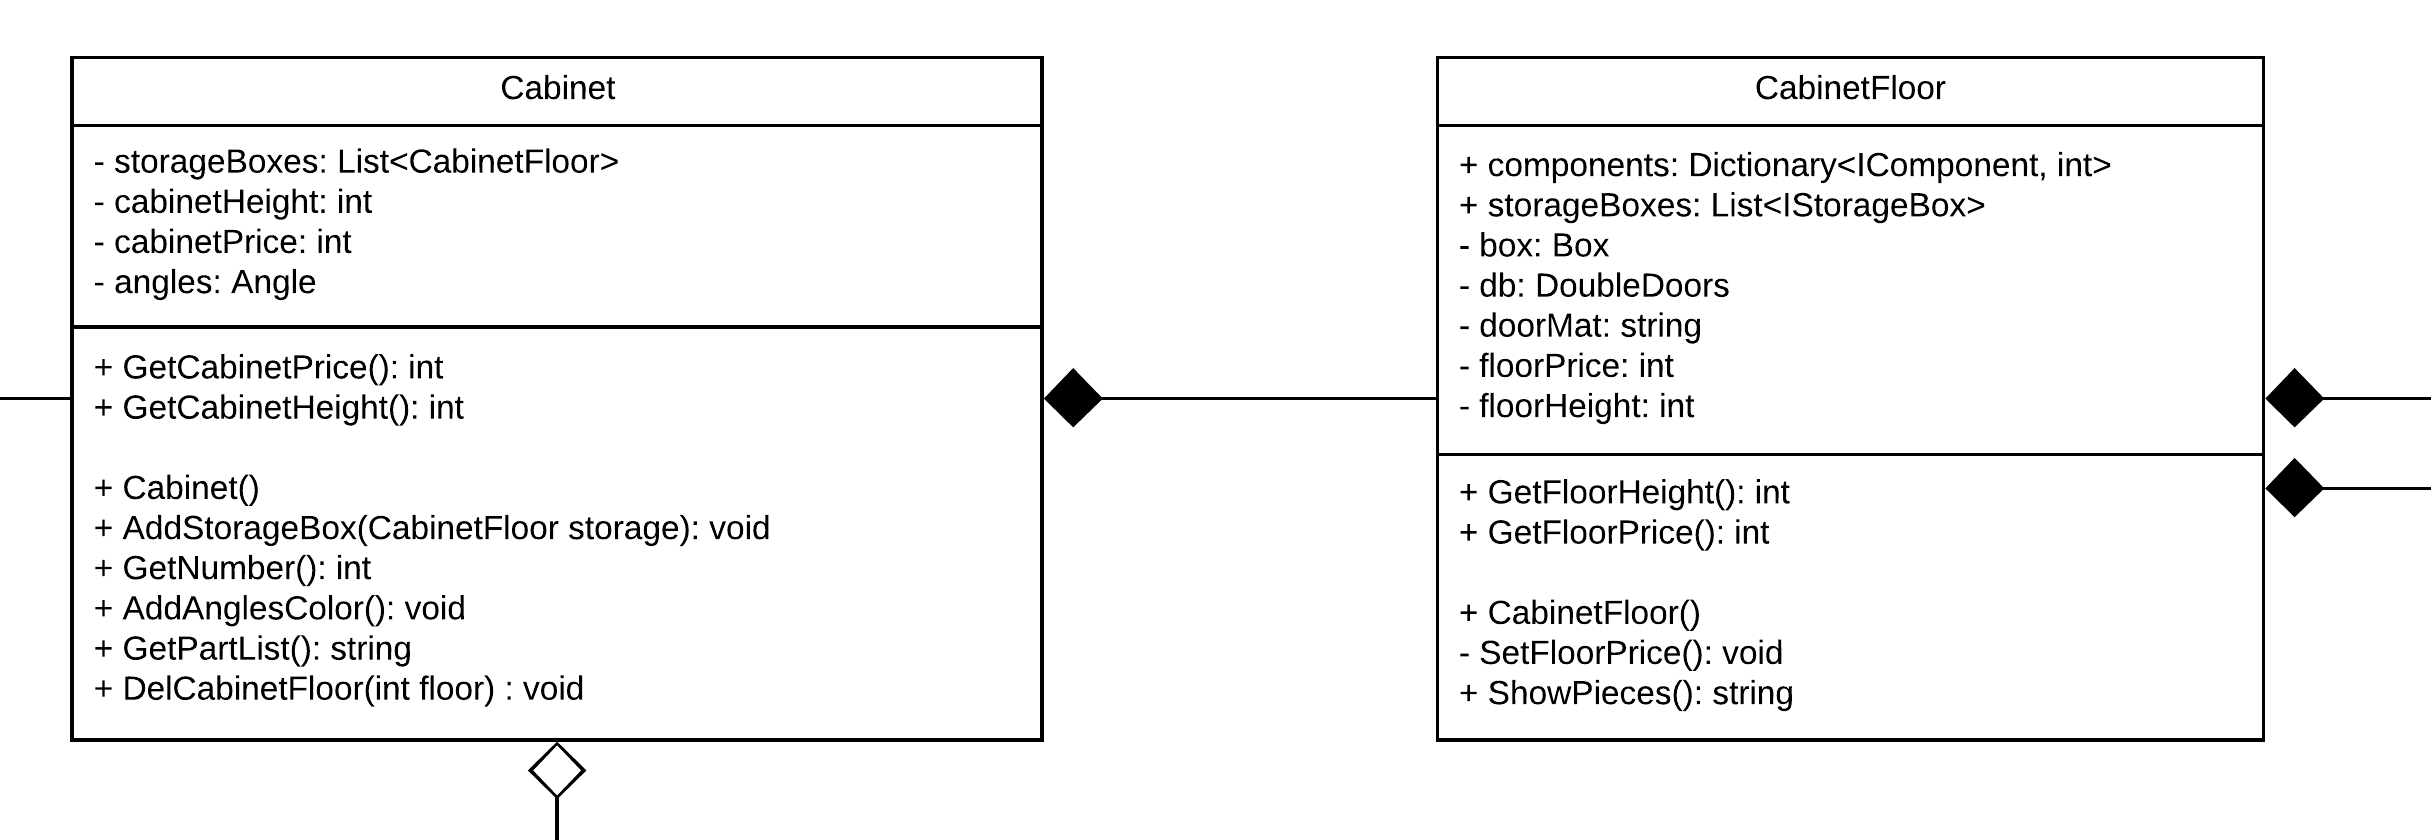
\includegraphics[width = 0.65\textwidth]{Figures/CabinetClass.png}
			\caption{Class Cabinet and CabinetFloor}
			\label{cabinetclass}
		\end{figure*} 
		
        \paragraph{}
        Regarding the technology, we chose to develop our application in C\# and our interface is made using a Windows Form. There are two interfaces, the first one for the customer, which enables him to create and order a cabinet. The second one has been developed for the storekeeper where he can access the database to see the stock and close orders. We chose to use Windows Form because of its easy interface generation and pre-coded elements.
 
    \newpage
    \subsection{Entity - relation}
        \vspace{\baselineskip}
        
        \begin{figure*}[h!]
            \centering
			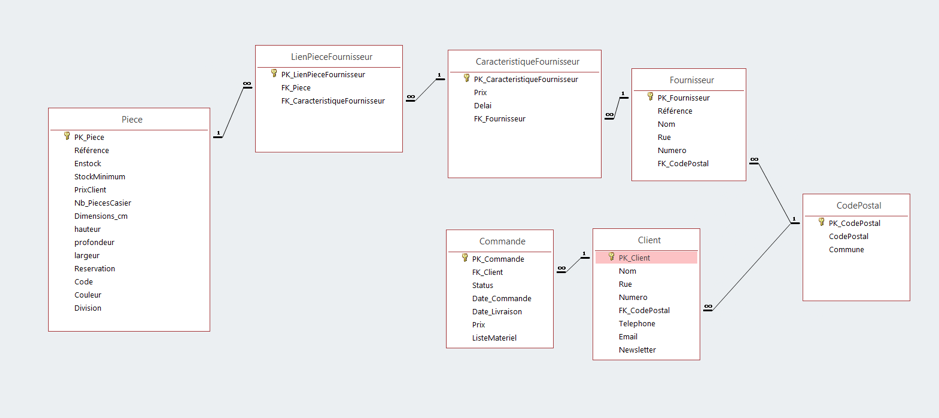
\includegraphics[width = 1\textwidth]{Figures/EntityRelation.png}
			\caption{Entity-Relation Diagram}
			\label{entityrelation}
		\end{figure*} 
		
        \paragraph{}
        There are two parts in this diagram, a first one about the parts and their suppliers and a second one where we can find the tables containing the client and the order.
        
        \paragraph{}
        To make our database, we used Access, but first, we began with the excel from the customer, which we separated in multiple spreadsheets. These different spreadsheets are the tables that you can see on the diagram ( Piece, LienPieceFournisseur...) in them we added the characteristics which are in relation with the title of the table.  
        
        \paragraph{}
        So in "Piece" you will find all the properties to identify the different parts of the shelf, in "LienPieceFournisseur" you have the different foreigner keys which allow not to duplicate data in our database and just have a table which makes the link between the parts characteristics and the supplier. For one part you can have more than one supplier. It is the same for the Zip code; we have only one table which has a link with the supplier and the client, so we do not duplicate data. 
        
        \paragraph{}
        We wanted something simple and easy to deal with, so there is no 1 to 1 relation only 1 to infinite, therefore, we have a short amount of table and no purely unnecessary table.
        
\newpage
\section{User Interface}
Images of the user interface are available in Appendix \ref{AppendixA} section \ref{Userinterface}, please refer to help you understand the following explanations. 
    \subsection{Dashboard and homepage}
        \paragraph{}
        When you start the application, you are welcomed by a homepage with a carousel containing pictures of kitbox cabinets. (Under that carousel, we made a label box available so that the client can put a welcoming word for the user, or something else). This carousel works with a timer and a method that loops through images located in the bin/debug/image folder.
        
        \paragraph{}
        On the left hand side of the the user interface, you can find a navigation bar. We decided to make our user interface like a website. What we mean by that is that we are playing with the visibility to show the different pages. You can go through the various pages using this navigation bar as its name indicates. 
        
        \vspace{\baselineskip}

        \textbf{How did we proceed?}
        
        \paragraph{}
        As we decided to work with the .NET framework, our graphical interface is a winform. This winform can include multiple forms and it is possible to navigate between them. We decided to use an alternative way to multiple forms and used an one and only form which contains in his initial state the dashboard elements.
        
        We divide the dashboard into four parts : 
        
        \begin{itemize}
            \item The upper part is providing the logo and the name of our client's company.
            \item The bottom part is not very important.
            \item The section on the left side is the navigation bar.
            \item The centre block which will incorporate the content of different pages we have made available.
        \end{itemize}
        
        \paragraph{}
        The centre block will thus contain the actual content of our user interface. This alternative way makes us use user controls, which are used to group a set of controls and behaviours in a reusable way. You can not show a user control on the screen unless it's added to a form somewhere. By using those user controls, it enabled us to structure our code and pass on information more easily from one page to another. What makes it more structured? Each user control has his own code, and thus, it separates each part from each other, which makes it easier to modify the code for a specific feature/page.
        
        \newpage
        The navigation bar contains multiple buttons enabling the navigation between the different parts of the application. As you can see on Figure \textit{\ref{fig:navigationBar}}, it enables the user to navigate between the "Dashboard", "Creation", "Cart" and "About Us" pages.
        
        \begin{figure}[h!]
            \centering
			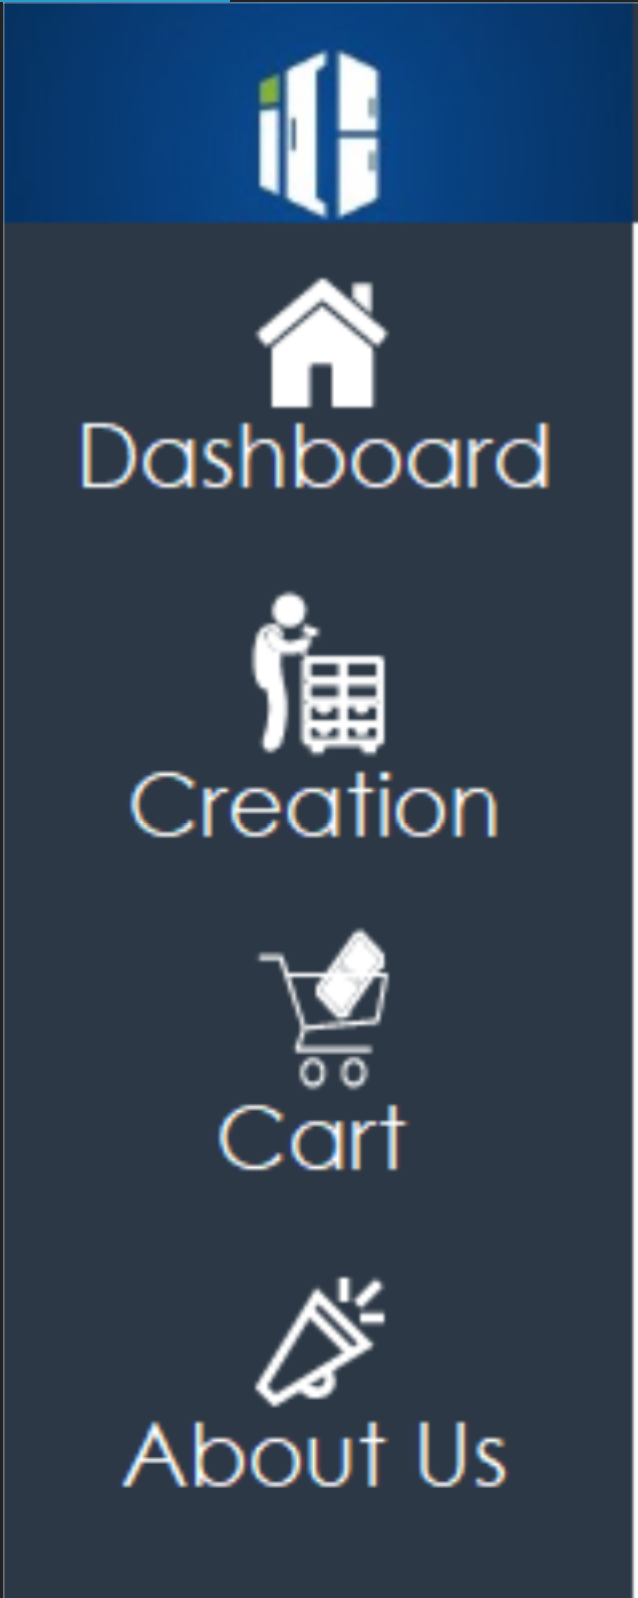
\includegraphics[width = 0.25\textwidth]{Figures/navigationBar.PNG}
            \caption{Navigation bar of user interface}
            \label{fig:navigationBar}
        \end{figure}
        
        \paragraph{}
        As we move into the navigation bar, the second tab is “Creation”. 
        \vspace{\baselineskip}
        \vspace{\baselineskip}
        
    \subsection{Creation}
        \paragraph{}
        You are welcomed with a little message explaining the two different kinds of creation the user can choose from. The two options are the following : 
        
        \begin{itemize}
            \item Creation from scratch: which enables the user to be completely free in his choice of box dimensions.
            \item Creation from standard dimensions: which allows the user to choose from standard sizes for the cabinet. All the boxes are of the same height.
        \end{itemize}
        \vspace{\baselineskip}
        
        When the user has chosen his creation mode, the user arrives on the specific creation page. He can still select the other method in a user-friendly way if he wants to.

        \newpage
    
        \subsubsection{Creation from scratch}
            \paragraph{}
            As we said, the user has more freedom in this part, with a little supplement to pay, as each box of the cabinet can have different heights. This creation enables also to make higher cabinets.
            
            \paragraph{}
            As you can see on figure \textit{\ref{fig:CommonBoxFeatures}}, first the user is asked how much boxes he wants his cabinet to have. After that, he needs to choose the colour of the angles, the depth and the width of the cabinet, as the boxes cannot vary in those dimensions in one cabinet. 
            
            \begin{figure}[h!]
                \centering
    			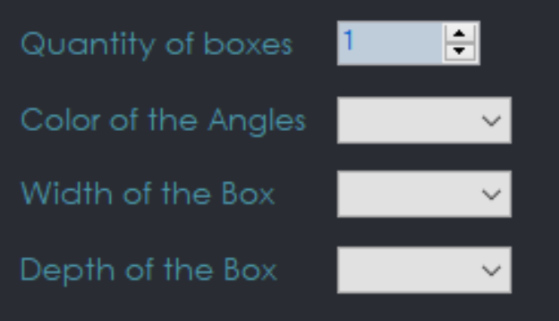
\includegraphics[width = 0.4\textwidth]{Figures/CommonBoxFeatures.PNG}
                \caption{Creation form scratch first parameters}
                \label{fig:CommonBoxFeatures}
            \end{figure}
            
            \paragraph{}
            As you add new boxes, thus increment the number of boxes you want, a new tab page is added, containing the specific features for each box of the cabinet like shown on Figure \textit{\ref{fig:creationTabPage}}. The user will, therefore, be able to choose the height and colour of the box-level of the assembly he is creating. In that same tab page, he will be asked if he wants a door for that floor. If the user has chosen a door, the colour and materials he has opted for will be displayed. 
            \vspace{\baselineskip}
            \begin{figure}[h!]
                \centering
    			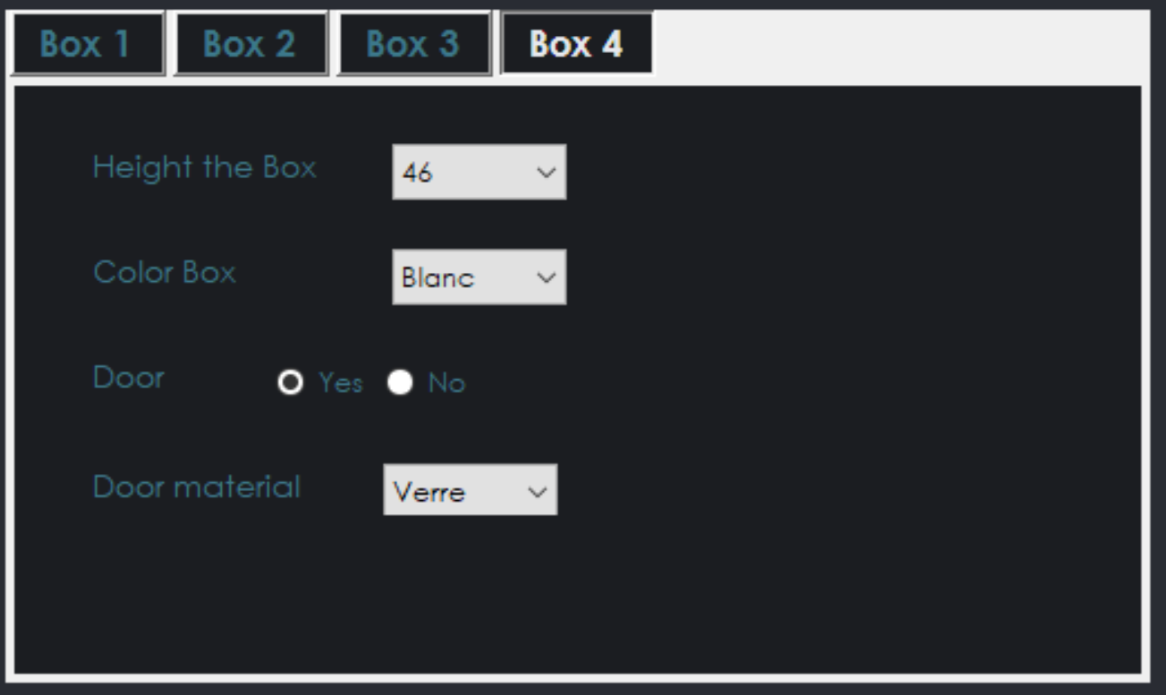
\includegraphics[width = 0.7\textwidth]{Figures/CreationTabPages.PNG}
                \caption{Creation form scratch box specific parameters}
                \label{fig:creationTabPage}
            \end{figure}
            
            \paragraph{}
            As you may have seen, a picture of the box is displayed on the right side to enable the user to have an idea of what it will look like. As the user makes his choices, the cabinet image will update itself depending on the box quantity, colour and door material of each box. 
            
            \paragraph{}
            A numeric up-down box gives the number of boxes. The rest of the choices are made available in combo boxes containing data coming from the database. We load those data via SQL request commands filtering the needed possibilities available for the specific features. Then they are loaded in each combo box when the user control is created.
            
            In \textit{Figure \ref{fig:loaddataheight}} you can find an example loading the data in the height combo boxes. 
            \vspace{\baselineskip}
            \begin{figure}[h!]
                \begin{minted}[
frame=lines,
framesep=2mm,
baselinestretch=1.2,
fontsize=\footnotesize,
linenos
]
{csharp}

// Loading Height data from data base
private void LoadDataBoxHeight()
{
    System.Windows.Forms.ComboBox[] list = {
        comboBoxHeight1,
        comboBoxHeight2,
        comboBoxHeight3,
        comboBoxHeight4,
        comboBoxHeight5,
        comboBoxHeight6,
        comboBoxHeight7
    };
    LoadDataGeneralForHeight(list, "SELECT DISTINCT hauteur FROM Piece WHERE" + 
                             "référence LIKE 'PA%' AND référence NOT LIKE 'PAH%' ");
}
\end{minted}
                \caption{Method retrieving the different combobox using same data and loading that data in the comboboxes}
                \label{fig:loaddataheight}
            \end{figure} 
            
            \paragraph{}
            On the other hand the \textit{Figure \ref{fig:loaddata}} shows the method called when the page ‘creation from scratch’ is loaded for the first time. As you can see the load method is called containing two parameters, the list of comboboxes the interface has to load and the SQL command to load the specific data needed from the database. This method will try to load the data by first clearing the comboboxes, execute the SQL command and store the retrieved data. Then it will for each combobox, load the stored data.
            \vspace{\baselineskip}
            \newpage
            
            \begin{figure}[h!]
                \begin{minted}[
frame=lines,
framesep=2mm,
baselinestretch=1.2,
fontsize=\footnotesize,
linenos
]
{csharp}

// function model for loadData
private void LoadDataGeneral(System.Windows.Forms.ComboBox[] m, string n)
{
    foreach (System.Windows.Forms.ComboBox i in m)
    {
        i.Items.Clear();
    }
    try
    {
        string q = n;
        cmd.CommandText = q; // execution of a SQL instruction
        cn.Open();
        dr = cmd.ExecuteReader();
        if (dr.HasRows)
        {
            while (dr.Read())
            {
                foreach (System.Windows.Forms.ComboBox i in m)
                {
                    i.Items.Add(dr[0].ToString());
                }
            }
        }
        dr.Close();
        cn.Close();
    }
    catch (Exception e)
    {
        cn.Close();
        MessageBox.Show(e.Message.ToString());
    }
}
\end{minted}
                \caption{Method enabling the loading and charging of data from the database using oledb}
                \label{fig:loaddata}
            \end{figure}

            \paragraph{}
            The door feature is made of a radio button and a combobox. This radio button will cause the combo box to be visible or not, according to the choice the user makes. At the same time, the door will be added or removed from the image. The code on \textit{Figure \ref{fig:loadImage}} shows how the colour and doors of the boxes on the cabinet's image are updated. There is a set of images available in the resources. Each one is named after the colour and door material of the box. If the user chooses to add at least one door to his cabinet, he will need to re-select a new width as not all width are available with doors, if he had already chosen a width.
            
            \paragraph{}
            \begin{figure}[h!]
                \begin{minted}[
frame=lines,
framesep=2mm,
baselinestretch=1.2,
fontsize=\footnotesize,
linenos
]
{csharp}
// general function to add color to box cabinet image
private void AddColorOrDoorToBox(ComboBox box, ComboBox door, WinFormPanel shelf)
{
    string color = box.Text;
    // in case color reset to null (initial state is white)
    if (color == "")
    {
        color = "blanc";
    }
    if (door.Text == "")
    {
        Image myImage = new Bitmap(
            GetRelativePath(Path.Combine(AppDomain.CurrentDomain.BaseDirectory)) +
            @"Documents\GitHub\Projet_KitBox\Interface\KitBoxApplication\" + 
            "KitBoxApplication\Resources\" + color + "NoDoor.png");
        shelf.BackgroundImage = myImage;
    }
    else
    {
        string doorMat = door.Text;
        Image myImage = new Bitmap(
            GetRelativePath(Path.Combine(AppDomain.CurrentDomain.BaseDirectory)) +
            @"Documents\GitHub\Projet_KitBox\Interface\KitBoxApplication\" + 
            "KitBoxApplication\Resources\" + color + doorMat + ".png");
        shelf.BackgroundImage = myImage;
    }
}
\end{minted}
                \caption{Method loading the right image for the box from the properties selected}
                \label{fig:loadImage}
            \end{figure}
            
            \paragraph{}
            Although the height of each box is free, there is still a max height that can not be exceeded. To prevent the user exceeding it, we displayed a box giving a real-time report of the height the cabinet. This height will be shown in green if the maximum height has not been exceeded yet and in red if it is exceeded as shown on \textit{Figure \ref{fig:maxHeight}}. If the user still tries to make a cabinet with a height exceeding the maximum, a message box will appear asking the user to change some of the heights of their boxes to reduce the total height of the cabinet.
            \vspace{\baselineskip}
            
            \begin{figure*}[h!]
                \centering
    			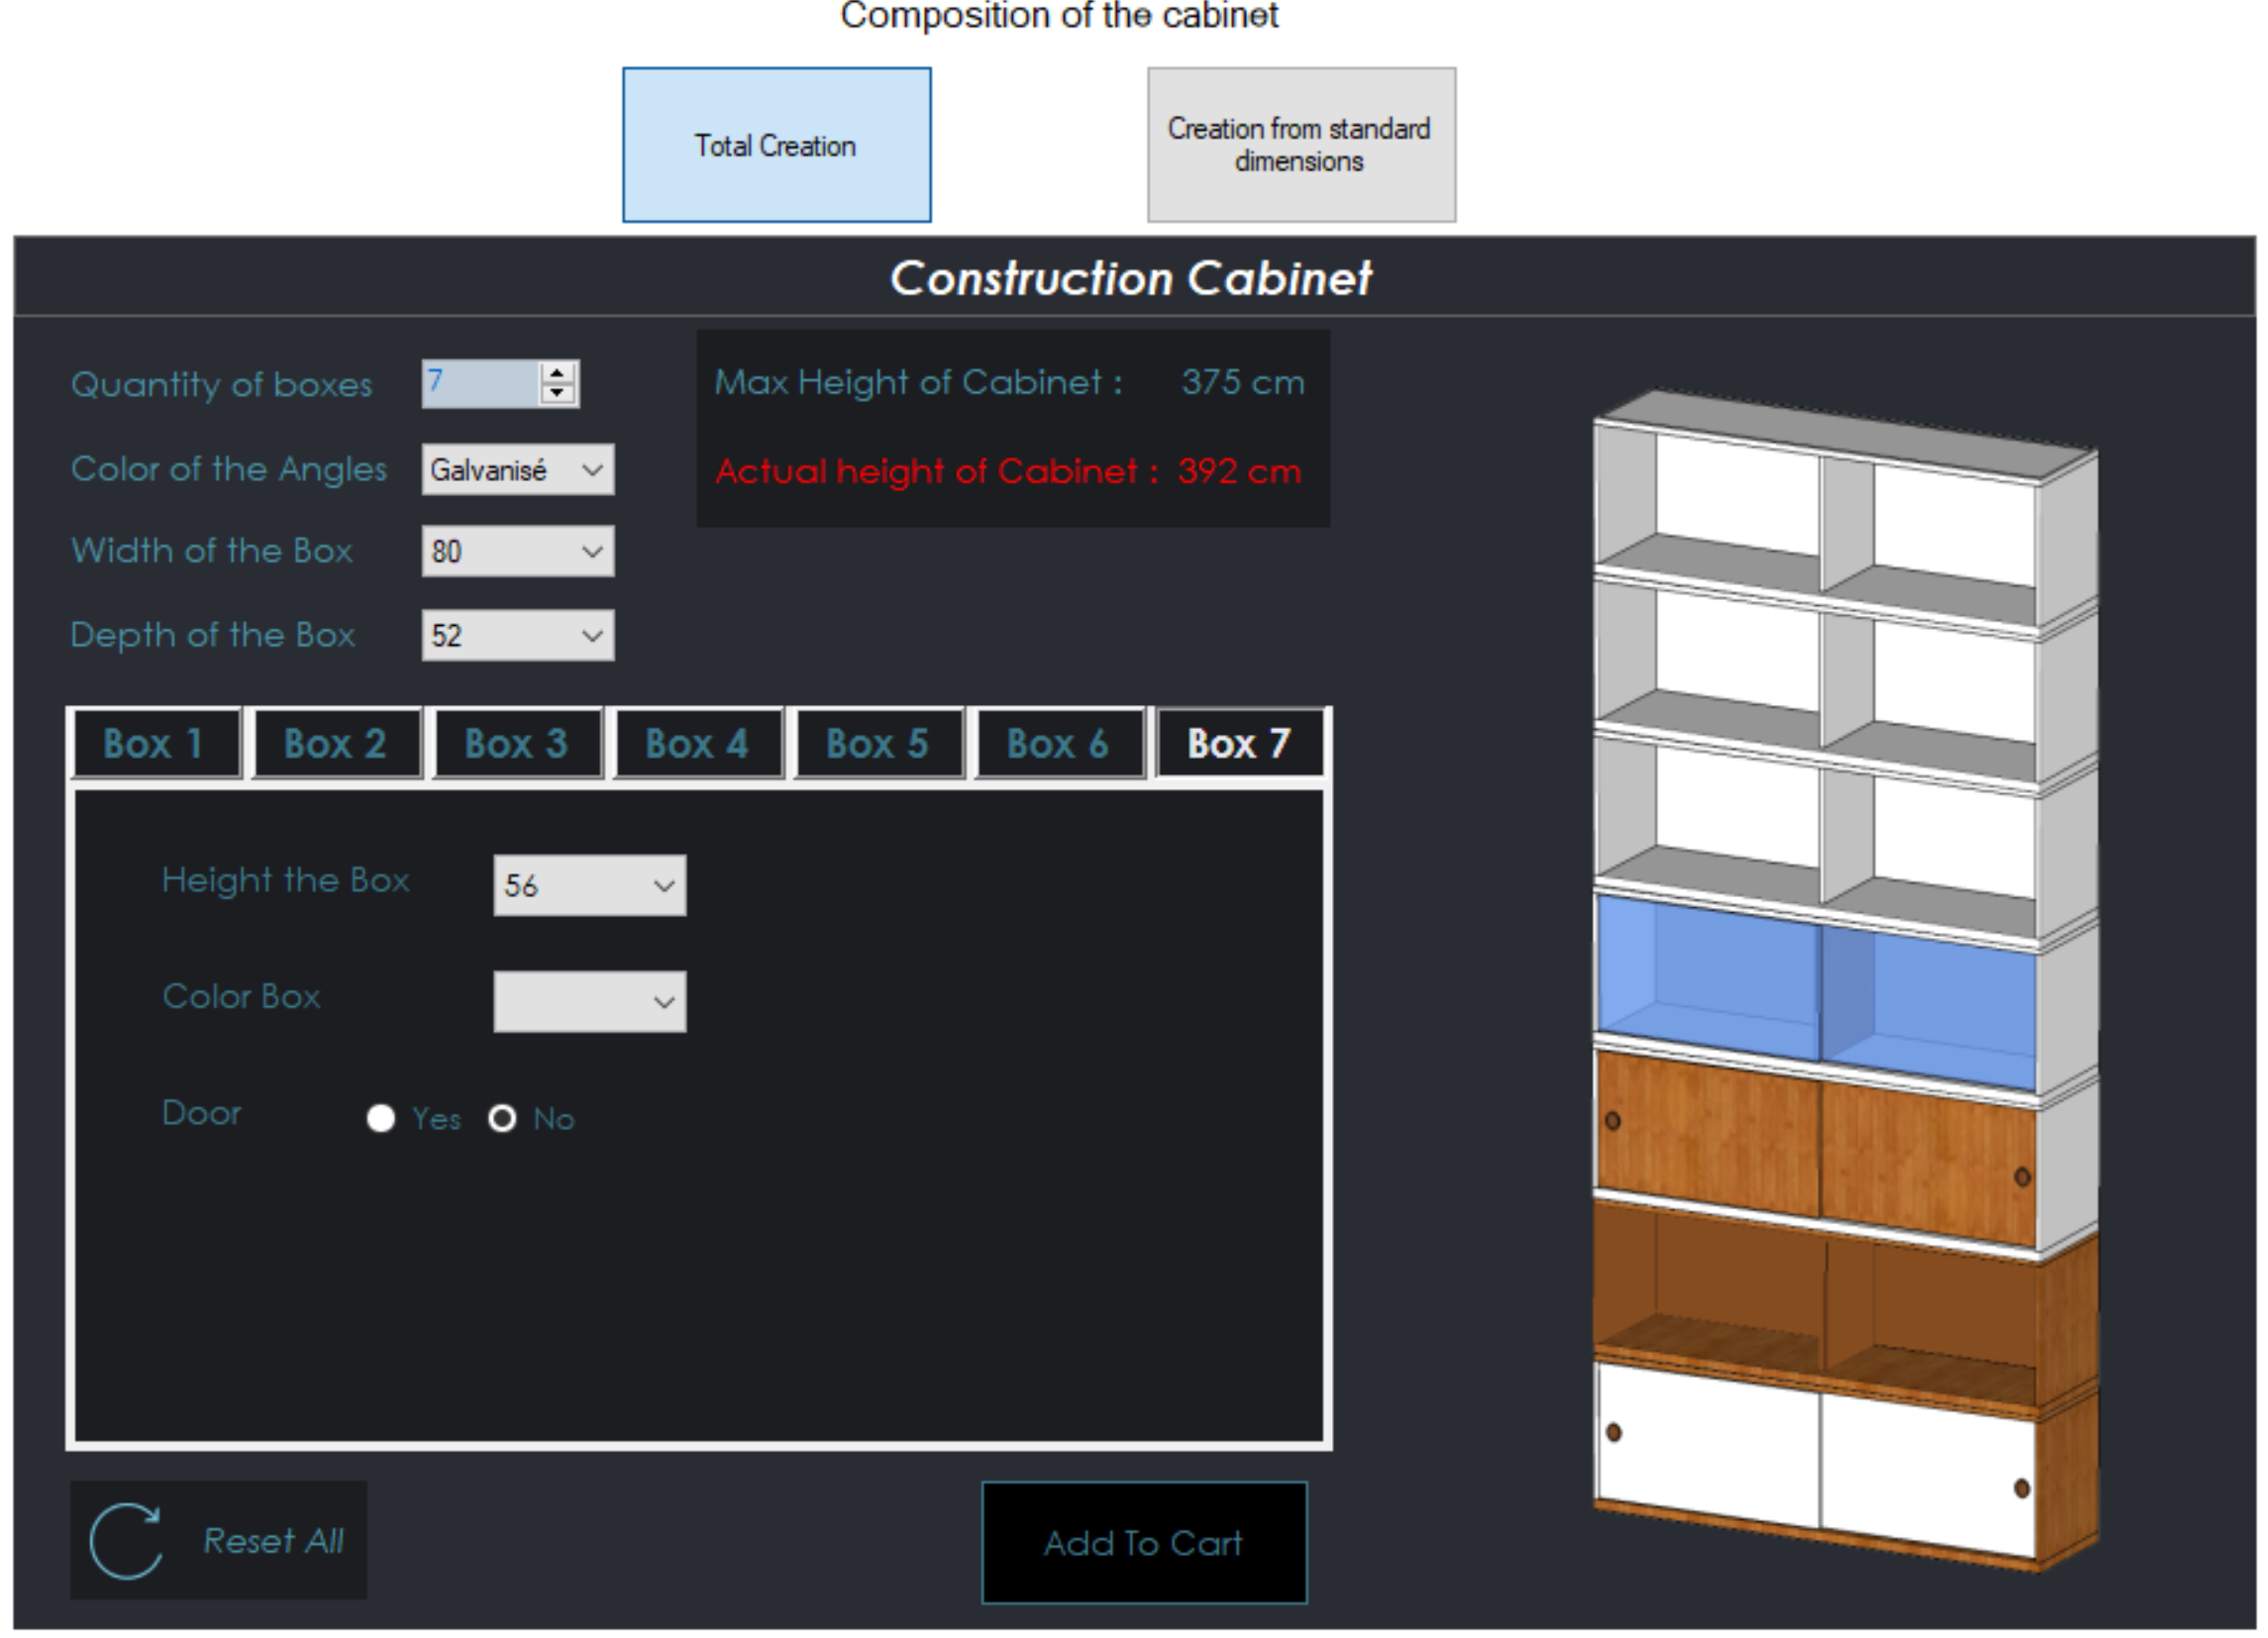
\includegraphics[width = 1\textwidth]{Figures/CreationScratchHeight.PNG}
    			\caption{Creation From Scratch Interface exceeding maximum height}
    			\label{fig:maxHeight}
    		\end{figure*}
            \vspace{\baselineskip}
            
            At last, there are two buttons : 
            \begin{itemize}
                \item “Reset All” button: which resets every combobox, numericupdown and radio button to its initial state.
                \item “Add to Cart” button: which adds the cabinet the user has composed to the cart.
            \end{itemize}
            \vspace{\baselineskip}
            
            Three different outcomes are possible : 
            \begin{itemize}
                \item A message telling the user the maximum height has been exceeded 
                \item A message telling the user to fill every empty combo box 
                \item A loading bar showing that the cabinet is being created
            \end{itemize}
            \vspace{\baselineskip}
            
            This last outcome was needed because each construction of our cabinet takes a certain time. To show the user the cabinet is being processed, we added a loading bar. This loading bar was only possible by using a background worker. We made a method that initiates a background worker and shows this loading bar. This method is charged for each box and meanwhile, when a box is finished, as shown on \textit{Figure \ref{fig:LoadingBar}}, the progress bar fills itself.
            \vspace{\baselineskip}
            \vspace{\baselineskip}
            
            \begin{figure*}[h!]
                \centering
    			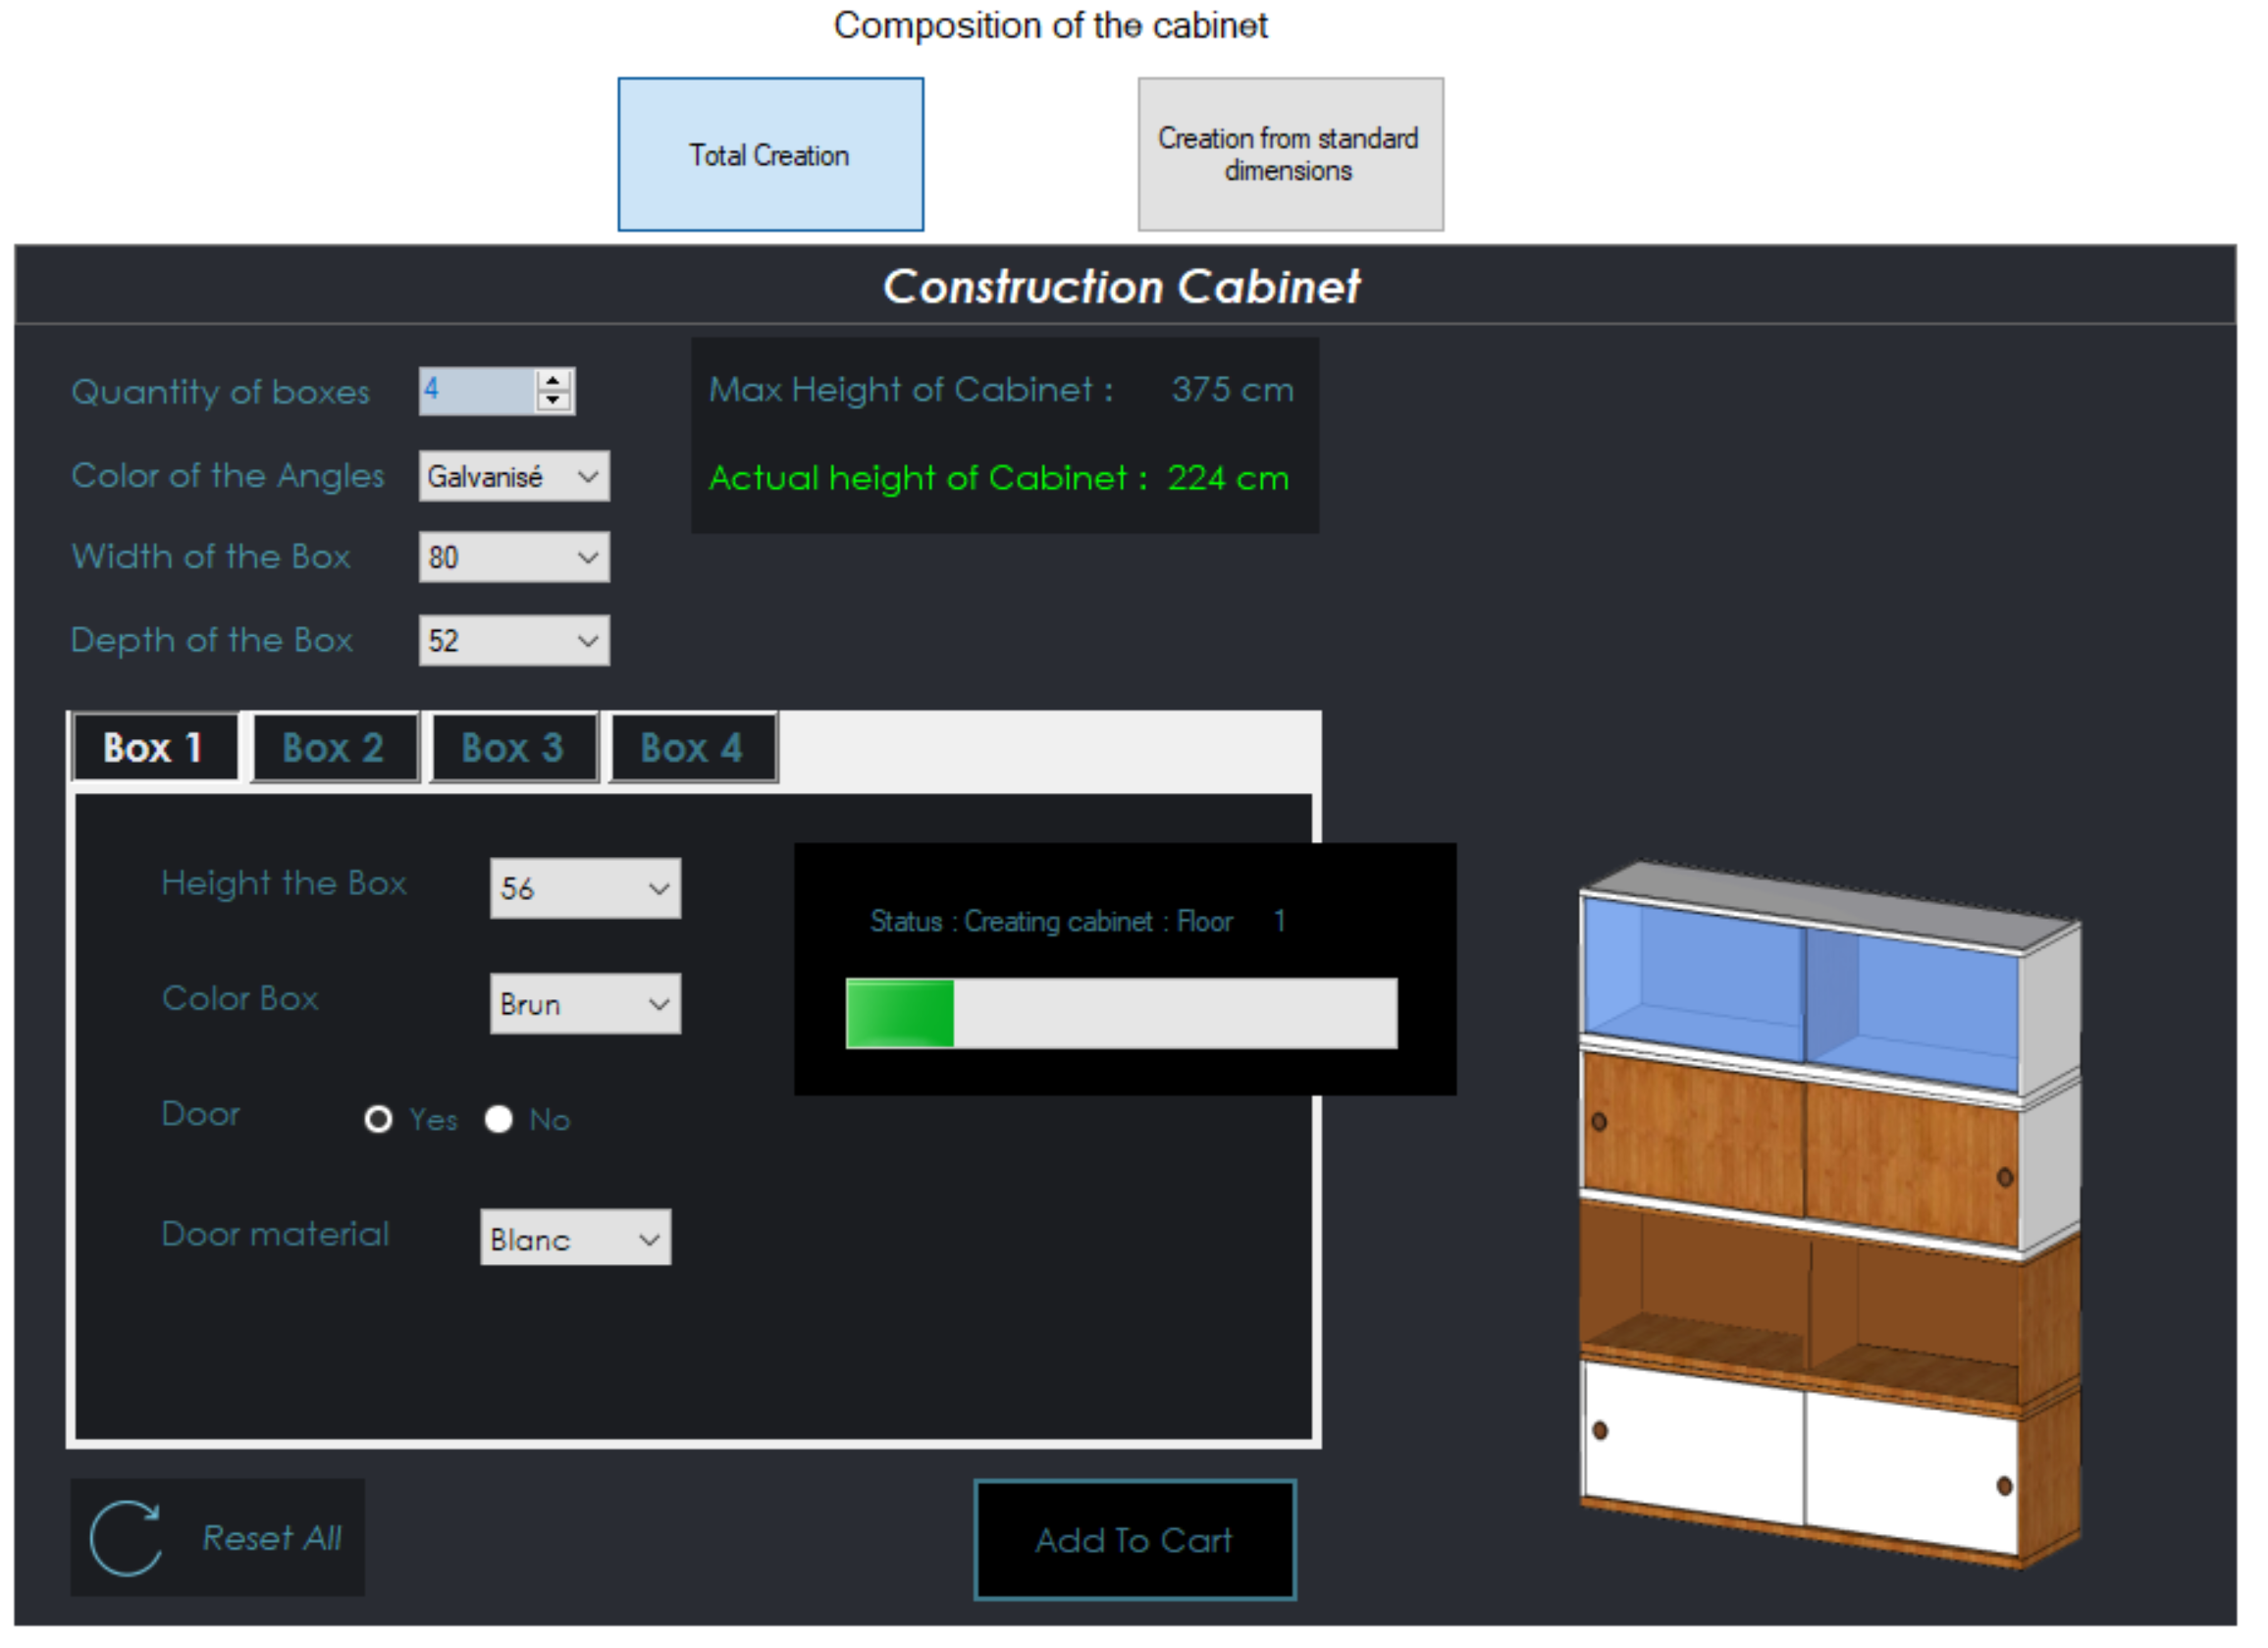
\includegraphics[width = 1\textwidth]{Figures/CreationScratchLoading.PNG}
    			\caption{Creation From Scratch Interface loading bar}
    			\label{fig:LoadingBar}
    		\end{figure*}
            \vspace{\baselineskip}
        
        \newpage
        \subsubsection{Creation from standard dimension}
            \paragraph{}
            If the user choose the other type of creation, he will only be able to choose from a set of prefixed heights for the cabinets as shown on \textit{Figure \ref{fig:fixedheight}}. 
            \vspace{\baselineskip}
            
            \begin{figure*}[h!]
                \centering
    			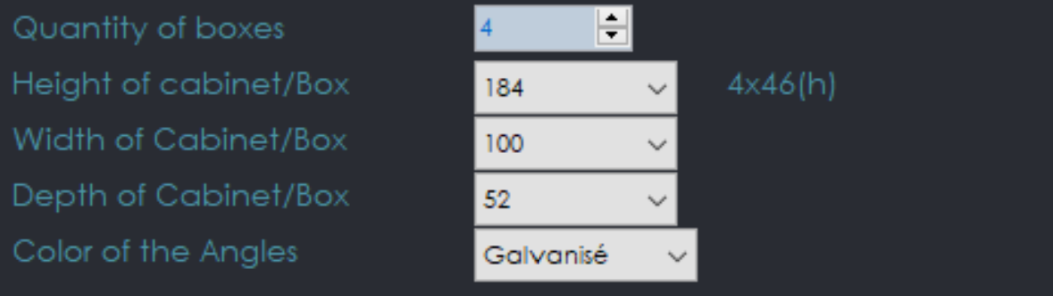
\includegraphics[width = 0.7\textwidth]{Figures/boxHeight.PNG}
    			\caption{Creation from standard dimensions with fixed height}
    			\label{fig:fixedheight}
    		\end{figure*}
            
            \paragraph{}
            As you can see, the user is first asked to choose the number of boxes he wants his cabinet to have.  Then he is asked to choose the height of cabinet. The values of those heights are updated each time the user changes the number of boxes he wants. Next to the combobox containing the cabinet height, the actual height of the boxes is displayed after selecting a height. Again, same as in the creation from scratch, the user is asked to choose the width, depth and angle colour of the cabinet. 
            
            \paragraph{}
            An extra feature has been added to this creation, which is enabling the user to choose to give the same colour to all his boxes of the cabinet. According to his choice, he will choose one and only colour or a colour for each box. And again he will be able to choose if he wants a door to be added to the box-level of his choice. 
            
            \paragraph{}
            Apart from the check box enabling the choice for a common colour, we are using the same forms as for the ‘creation from scratch’, namely comboboxes, radio buttons and numeric up down. The method charged to make changes according to the value inside the numeric up down is more complex than in the ‘creation from scratch’. This is due to the design choice we made at the beginning. What makes this design more complex, is the code needed for the transition between 1 and multiple boxes.
            
            \paragraph{}
            As you can see on \textit{Figure \ref{fig:oneBox}} and on \textit{Figure \ref{fig:MultiBoxes}}, when it transits from one to more than one box, the colour and door choices disposition changes. As we found it would not have a good visual aspect to have a big space between the colour and door choice for one boxes, we decided to add an exclusive panel if only one box was chosen. For more than one box, all the forms for the colour and door choices are grouped in a same panel to enable an easier management of the visibility and a better structure.
            \newpage
            
             \begin{figure*}[h!]
                \centering
    			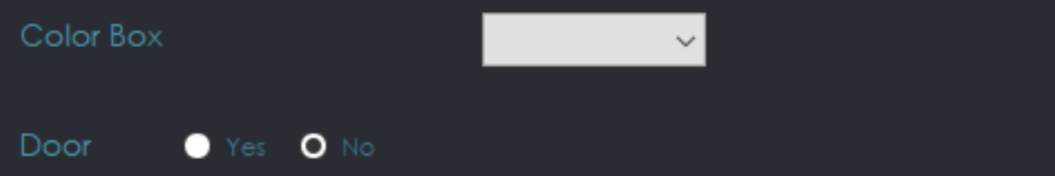
\includegraphics[width = 0.7\textwidth]{Figures/boxOne.PNG}
    			\caption{Creation from standard dimensions with one box}
    			\label{fig:oneBox}
    		\end{figure*}
    		\vspace{\baselineskip}
    		
    		 \begin{figure*}[h!]
                \centering
    			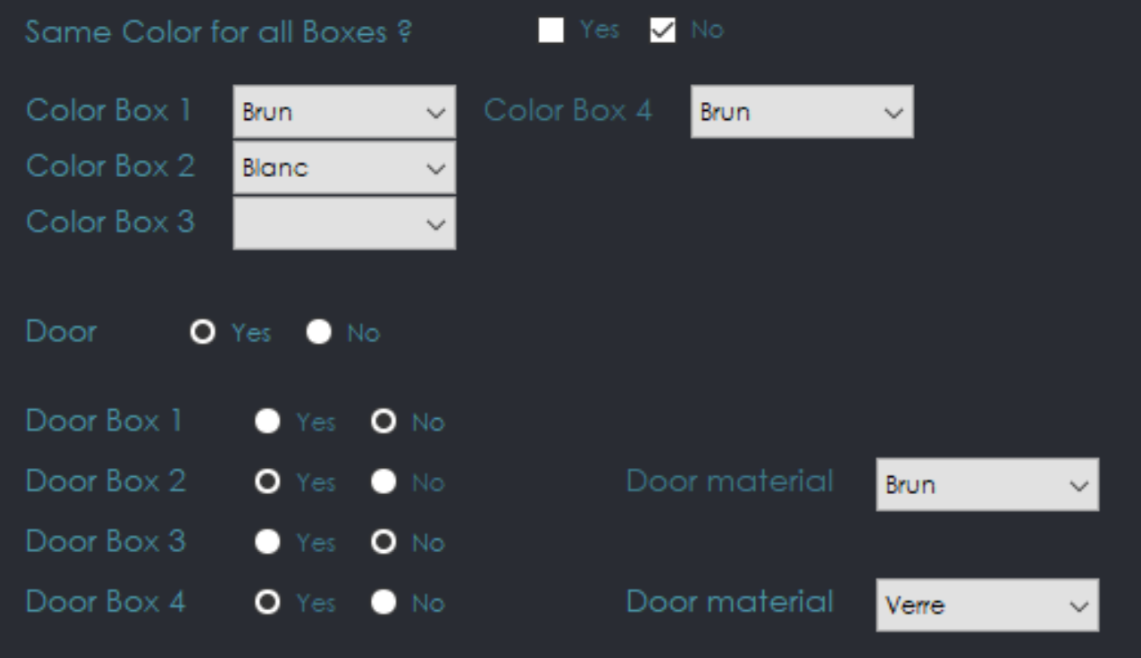
\includegraphics[width = 0.7\textwidth]{Figures/boxMultiple.PNG}
    			\caption{Creation from standard dimensions with multiple boxes}
    			\label{fig:MultiBoxes}
    		\end{figure*}
            
            \paragraph{}
            Thus, because of this design, the features chosen for the colour and door when one box is selected must be carried over to the new comboboxes that are being displayed if more than one box has been selected and vice versa. Besides that, it made it more difficult to manage the changes in the image of the cabinet. This part is thus definitely something that could be improved by using only one combobox for the colour and door of the first box or by taking the same design as the 'creation from scratch'.
            
            \paragraph{}
            The cabinet image rendition and the combobox data load is done in the same way as with the "creation from scratch" design. An extra method had to be added to enable having the same colour for each box. Again this design is also equipped with a “Reset” button and a “Add to cart” button. These two buttons are using kind of the same methods as for the “creation from scratch” design. Only difference here is that the max height cannot be exceeded. 
            
            And finally the outcomes are more or less the same too, except for the maximum height that cannot be exceeded.
           
    \newpage
    \subsection{Cart page}
        \paragraph{}
        When the customer is done with creating his own cabinets and as soon as he presses “Add to cart”, he will be able to access the cart page and see all the cabinets he created.
        \vspace{\baselineskip}
        
        \begin{figure*}[h!]
            \centering
    		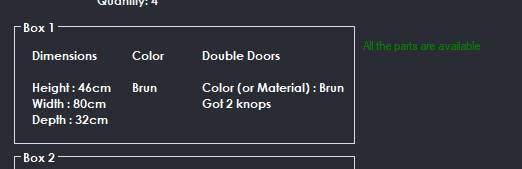
\includegraphics[scale=0.7]{Figures/AvailableLabel.PNG}
    		\caption{Storage box's description and availability label}
    		\label{avail}
    	\end{figure*}
    	
    	\paragraph{}
        As you can see in Figure \textit{\ref{carttab}}, the cart is designed so that the client can view each cabinet he created and review every storage box he has designed. For each cabinet, the colour, height, width, depth and angles’ length are displayed, then for each box level height, colour and door material is given too. Next to all the cabinet’s properties, a cabinet image is rendered in order to give a better idea of which cabinet the user is reviewing (\textit{Figure \ref{avail}} ).
        
        \begin{figure*}[h!]
            \centering
    		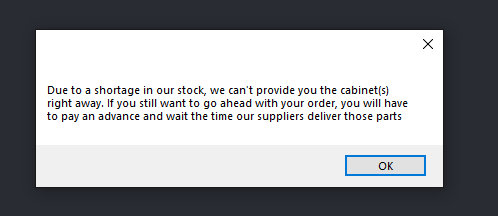
\includegraphics[scale=0.7]{Figures/ShortageMessage.PNG}
    		\caption{Notification of the missing parts}
    		\label{shortage}
    	\end{figure*}
    	
        \begin{figure*}[h!]
            \centering
    		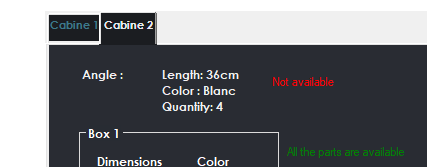
\includegraphics[scale=0.7]{Figures/UnavailibilityLabel.PNG}
    		\caption{Label for the missing part}
    		\label{unavail}
    	\end{figure*}
        
        \paragraph{}
        If a storage box’s part is missing in the company’s stock, the customer will get a message box, when entering the cart. This message box will tell the user some parts are missing and that he will have to wait until the company gets the missing parts in stock again (\textit{Figure \ref{shortage}} ). He will also be notified with a little label next to the concerned box (\textit{Figure \ref{unavail}} ). 
        
        \paragraph{}
        In case of errors appearing during creation or the user changing his mind, it is possible to delete a cabinet with the little button in the upper-right hand side. As for every cart, you can see the total price of this cart (\textit{Figure \ref{deleteButton}} ).
        \vspace{\baselineskip}
        
        \begin{figure*}[h!]
            \centering
    		
\includegraphics[scale=0.5]{Figures/DeleteButton.PNG}
    		\caption{Delete Button}
    		\label{deleteButton}
    	\end{figure*}

    	\paragraph{}
        Once the customer is satisfied with his cart, he just has to press the "Confirm cart" button to validate his cart. He will be redirected to a window where he is asked to enter his email address (\textit{Figure \ref{authtab}}). Therefore the company can keep track of his command. Admitting the customer enters a wrong text, the form won’t validate the order and he will be told it is incorrect. He is also given the choice to register to the newsletter. When confirmed, the cart will be send to the database and will be emptied for the next order.
    \vspace{\baselineskip}
    \vspace{\baselineskip}
       
    \subsection{About Us}
        \paragraph{}
        The last page we implemented is the “About Us” page, enabling our client, KitBox, to write a little bit about them in case any of their clients would be interested (\textit{Figure \ref{aboutus}}).
        \vspace{\baselineskip}

\newpage
\section{Storekeeper interface}
    \paragraph{}
    To fully understand the explanation below take the appendix \ref{Storekeeperinterface} in front of you.
   
    \subsection{Stock manager tab}
        \paragraph{}
        The first tab of this interface is the stock tab (\textit{Figure \ref{stocktab}}) where you find all the products and the stock that you currently have in storage. When you select an item, a blue link will appear in all the columns to have a good vision of each characteristics of the product, it is also used to fill the "Delete", "Update stock" and "Update Price" form. So you just need to modify the correspondent text box  by the new stock amount or the new price and then just click on update and it will be done. It is possible to delete a product from the database by selecting it and clicking on the Delete button.
    \vspace{\baselineskip}
        
    \subsection{New product or supplier tab}
        \paragraph{}
        In this tab (\textit{Figure \ref{suppliertab}}), the storekeeper is able to add to the database new products and supplier. To do it he just need to fill the form with all the information of the new product and by selecting the supplier in the table next to the form. If the supplier is not in it, he can be added by completing the second form.
        
        \paragraph{}
        The storekeeper has to select the zip code or by adding it to the list and it will fill the Zip Code text box. Then if he complete correctly the form, it will be added to the database and to the list for new product by clicking on the refresh button.
	\vspace{\baselineskip}
    \vspace{\baselineskip}
    
    \subsection{Order tab}
        \paragraph{}
        In one of the most important tab (\textit{Figure \ref{ordermanagertab}}) for the storekeeper, we find all the information about the orders except the complete list of the pieces to make the shelf. So when a client takes out his order, the storekeeper can give it by finding the correct order id and then he has to complete the order by filling the deliver date text box.
        
        \paragraph{}
        The order will go from the "in progress" table to the complete table with a certain amount of time because the system need to remove from the stock the parts of the order. The storekeeper can also delete a “in progress” order by selecting it and clicking on the Delete button.
        
    
    \newpage
    \subsection{Client tab}
        \paragraph{}
        The last tab (\textit{Figure \ref{clientmanagertab}}) is dedicated to the management of the clients. As you can see, the storekeeper has an overview of all the clients and he is able to add a new one by fulfilling the last grey square with their information. Like in the previous tab, there is a table with the zip code. So when he add a new client, the storekeeper has to select the zip code or add it to the table and it will fill in the Zip Code text box. Then by completing the form, the Client information table will refresh and display the new client in the list.
        
\newpage
\section{Conclusion}
    \paragraph{}
    In the end, our application works as expected. We developed a box creation tool which is capable of building a cabinet with all dimensions. Thanks to the interfaces and abstract class, it can be expanded in the future. We designed and created a modern user interface for both customer and  storekeeper. We also worked on the creation of a complete database and the integration of it in the application.
    
    \paragraph{}
    However, our application can be improved. For example, during the creation of the cabinet, we observed a long execution time due to all the SQL requests made in the background. Unfortunately,as we did not succeeded to solve it, we choose to inform the user by means of a progress bar.
    
    \paragraph{}
    A next major update that could have been done to the that interface is adding a catalogue page enabling the users to access quickly to the prices and available choices. In addition to that, it would allow our client to update their catalogue easily as the program would do it. This would need an update of the database, as the catalogue should be much more user friendly with images for each parts.
    
    \paragraph{}
    During our application's development, we choose to use some tools to help us. For safety and collaboration, we worked with GitHub. It allows us to work together at the same time without impacting each other's code. Also, it gives us an history of all the changes made.  While merging branches in GitHub, we encountered some difficulties due to code corruption or merge failure. This is caused by GitHub and old code version inside branches thus we had to fix them one by one.
    We also worked with Trello to manage our task and to check our progress in the project. We created a Discord server to communicate easier while we were not together. Thanks to screen sharing in Discord we could see the code of someone else to help him if needed.
    
    \paragraph{}
    In the beginning, we divided the work into parts. Some people worked on the user interface, while others on the database or the cabinet generation. When someone finished a task, he helped someone with their task. This method of collaboration helped us to speed up programming. In our group, we all had some facilities in some area of programming, so when we chose what we wanted to do, we were much more productive. When all the big parts where finished, we merged them all and made the finishing touch.
    
    \paragraph{}
    In conclusion, with this project, we developed our skills in object-oriented programming as well as in software engineering. We have discovered the power of WinForm and all the possibilities it offered to us. We learned how to work in a group and how to be organised. Moreover, we are proud of what we have accomplished together.


% Appendix A

\chapter{Appendix} % Main appendix title

\label{AppendixA} % For referencing this appendix elsewhere, use \ref{AppendixA}

%-----------------------------------
%	SECTION Python code
%-----------------------------------
\vspace{\baselineskip}
\vspace{\baselineskip}

\section{Glossary}
    \subsection{French}
        Acompte [\textit{Advance}] : paiement partiel à valoir sur le montant d'une somme due.\\
        AR [\textit{Back}] : arrière.\\
        Armoire [\textit{Cabinet}] : meuble permettant de stocker différents objets.\\
        AV [\textit{Front}] : avant.\\
        Casier [\textit{Storage box}] : sous partie de l’armoire. \\
        Clôturer [\textit{Close}] : finaliser, terminer une commande. \\
        Cornière [\textit{Angle}] : pièce verticale formant les coins de l’armoire. \\
        Coupelle [\textit{Knop}] : pièce de plastique placé sur la porte permettant d’agripper la porte et de la déplacer facilement. \\
        Facture [\textit{Bill-Invoice}] : pièce comptable par laquelle le vendeur fait connaître à l'acheteur le détail et le prix des marchandises vendues et services exécutés. \\
        Fournisseur [\textit{Supplier}] : personne/société qui fournit des marchandises de façon habituelle. \\
        GD [\textit{Left/Right}] : gauche - droite.\\
        HB [\textit{Up/Down}] : haut - bas.\\
        Magasinier [\textit{Storekeeper}] : employé s’occupant du magasin, du stock et des clients. \\
        Panneau [\textit{Panel}] : plaque de bois formant les parois de l’armoire.\\
        Parois [\textit{side}] :  côtés de l’armoire. \\
        Porte [\textit{Door}] : parois de bois ou de verre permettant de fermer le casier. \\
        Rainure [\textit{Groove}] : entaille longue dans une pièce permettant de faire passer la porte et de pouvoir la coulisser. \\
        Standardisées [\textit{Standardized}] : adjectif donner à un produit, une production à une norme, à un modèle unique. \\
        Tablettes [\textit{Shelf}] : plaque horizontale sur laquelle on peut poser divers objets. \\
        Tasseau [\textit{Cleat}] : petite pièce de bois destinée à soutenir l'extrémité d’un panneau. \\
        Tiroir [\textit{Drawer}] : Compartiment ouvert sur le haut, glissé dans un meuble. \\
        Traverse [\textit{Beam/Tie}] : pièce horizontale faisant partie de l’armature (arêtes) de l’armoire.
    
    \newpage
    \subsection{English}
        Advance [\textit{Acompte}]: partial payment on a total sum due.  \\
        Angle [\textit{Cornière}]: vertical part strengthening the cabinet’s corners. \\
        Back [\textit{AR}] \\
        Beam/Tie [\textit{Travèrse}]: horizontal part of the cabinet. It gives its strength to the cabinet. \\
        Bill [\textit{Facture}]: Accounting document by which the seller informs the buyer of the details and the price of the goods sold and services executed. \\
        Cabinet [\textit{Armoire}]: furniture to stock different objects. \\
        Cleat [\textit{Tasseau}]: small part made of wood supporting the extremity of a panel. \\
        Close [\textit{Clôturer}]: finalize, end an order.  \\
        Door [\textit{Porte}]: Wooden or glass plate allowing the storage box to be closed. 
        Down [\textit{HB}] \\
        Drawer [\textit{Tiroir}]: compartment opens on the upper side, slid into furniture. \\ 
        Front [\textit{AV}] \\
        Groove [\textit{Rainure}]: long cut in a part to place a sliding door. \\
        Invoice [\textit{Facture}]: Accounting document by which the seller informs the buyer of the details and the price of the goods sold and services executed. \\
        Knop [\textit{Coupelle}]: plastic part placed on the door to move it easier. \\
        Left [\textit{GD}] \\
        Panel [\textit{Panneau}]: wooden plate forming the cabinet’s wall. \\
        Right [\textit{GD}] \\
        Shelf [\textit{Tablette}]: horizontal plate to place objects. \\
        Side [\textit{Parois}]: cabinet or storage box wall. \\
        Standardized [\textit{Standardisée}]: adjective given to a product, a production with a norm or a unique model. \\
        Storage box [\textit{Casier}]: subpart of the cabinet. \\
        Storekeeper [\textit{Magasinier}]: Employee managing the store, the stock and the customers. \\
        Supplier [\textit{Fournisseur}]: person or company supplying regularly the commodity.\\ 
        Up [\textit{HB}]
%-----------------------------------
%	SECTION Python code
%-----------------------------------



\newpage
\section{Diagrams}
\label{diagrams}
    \subsection{Activity Diagram}
        \vfill
        \begin{figure*}[h!]
            \centering
			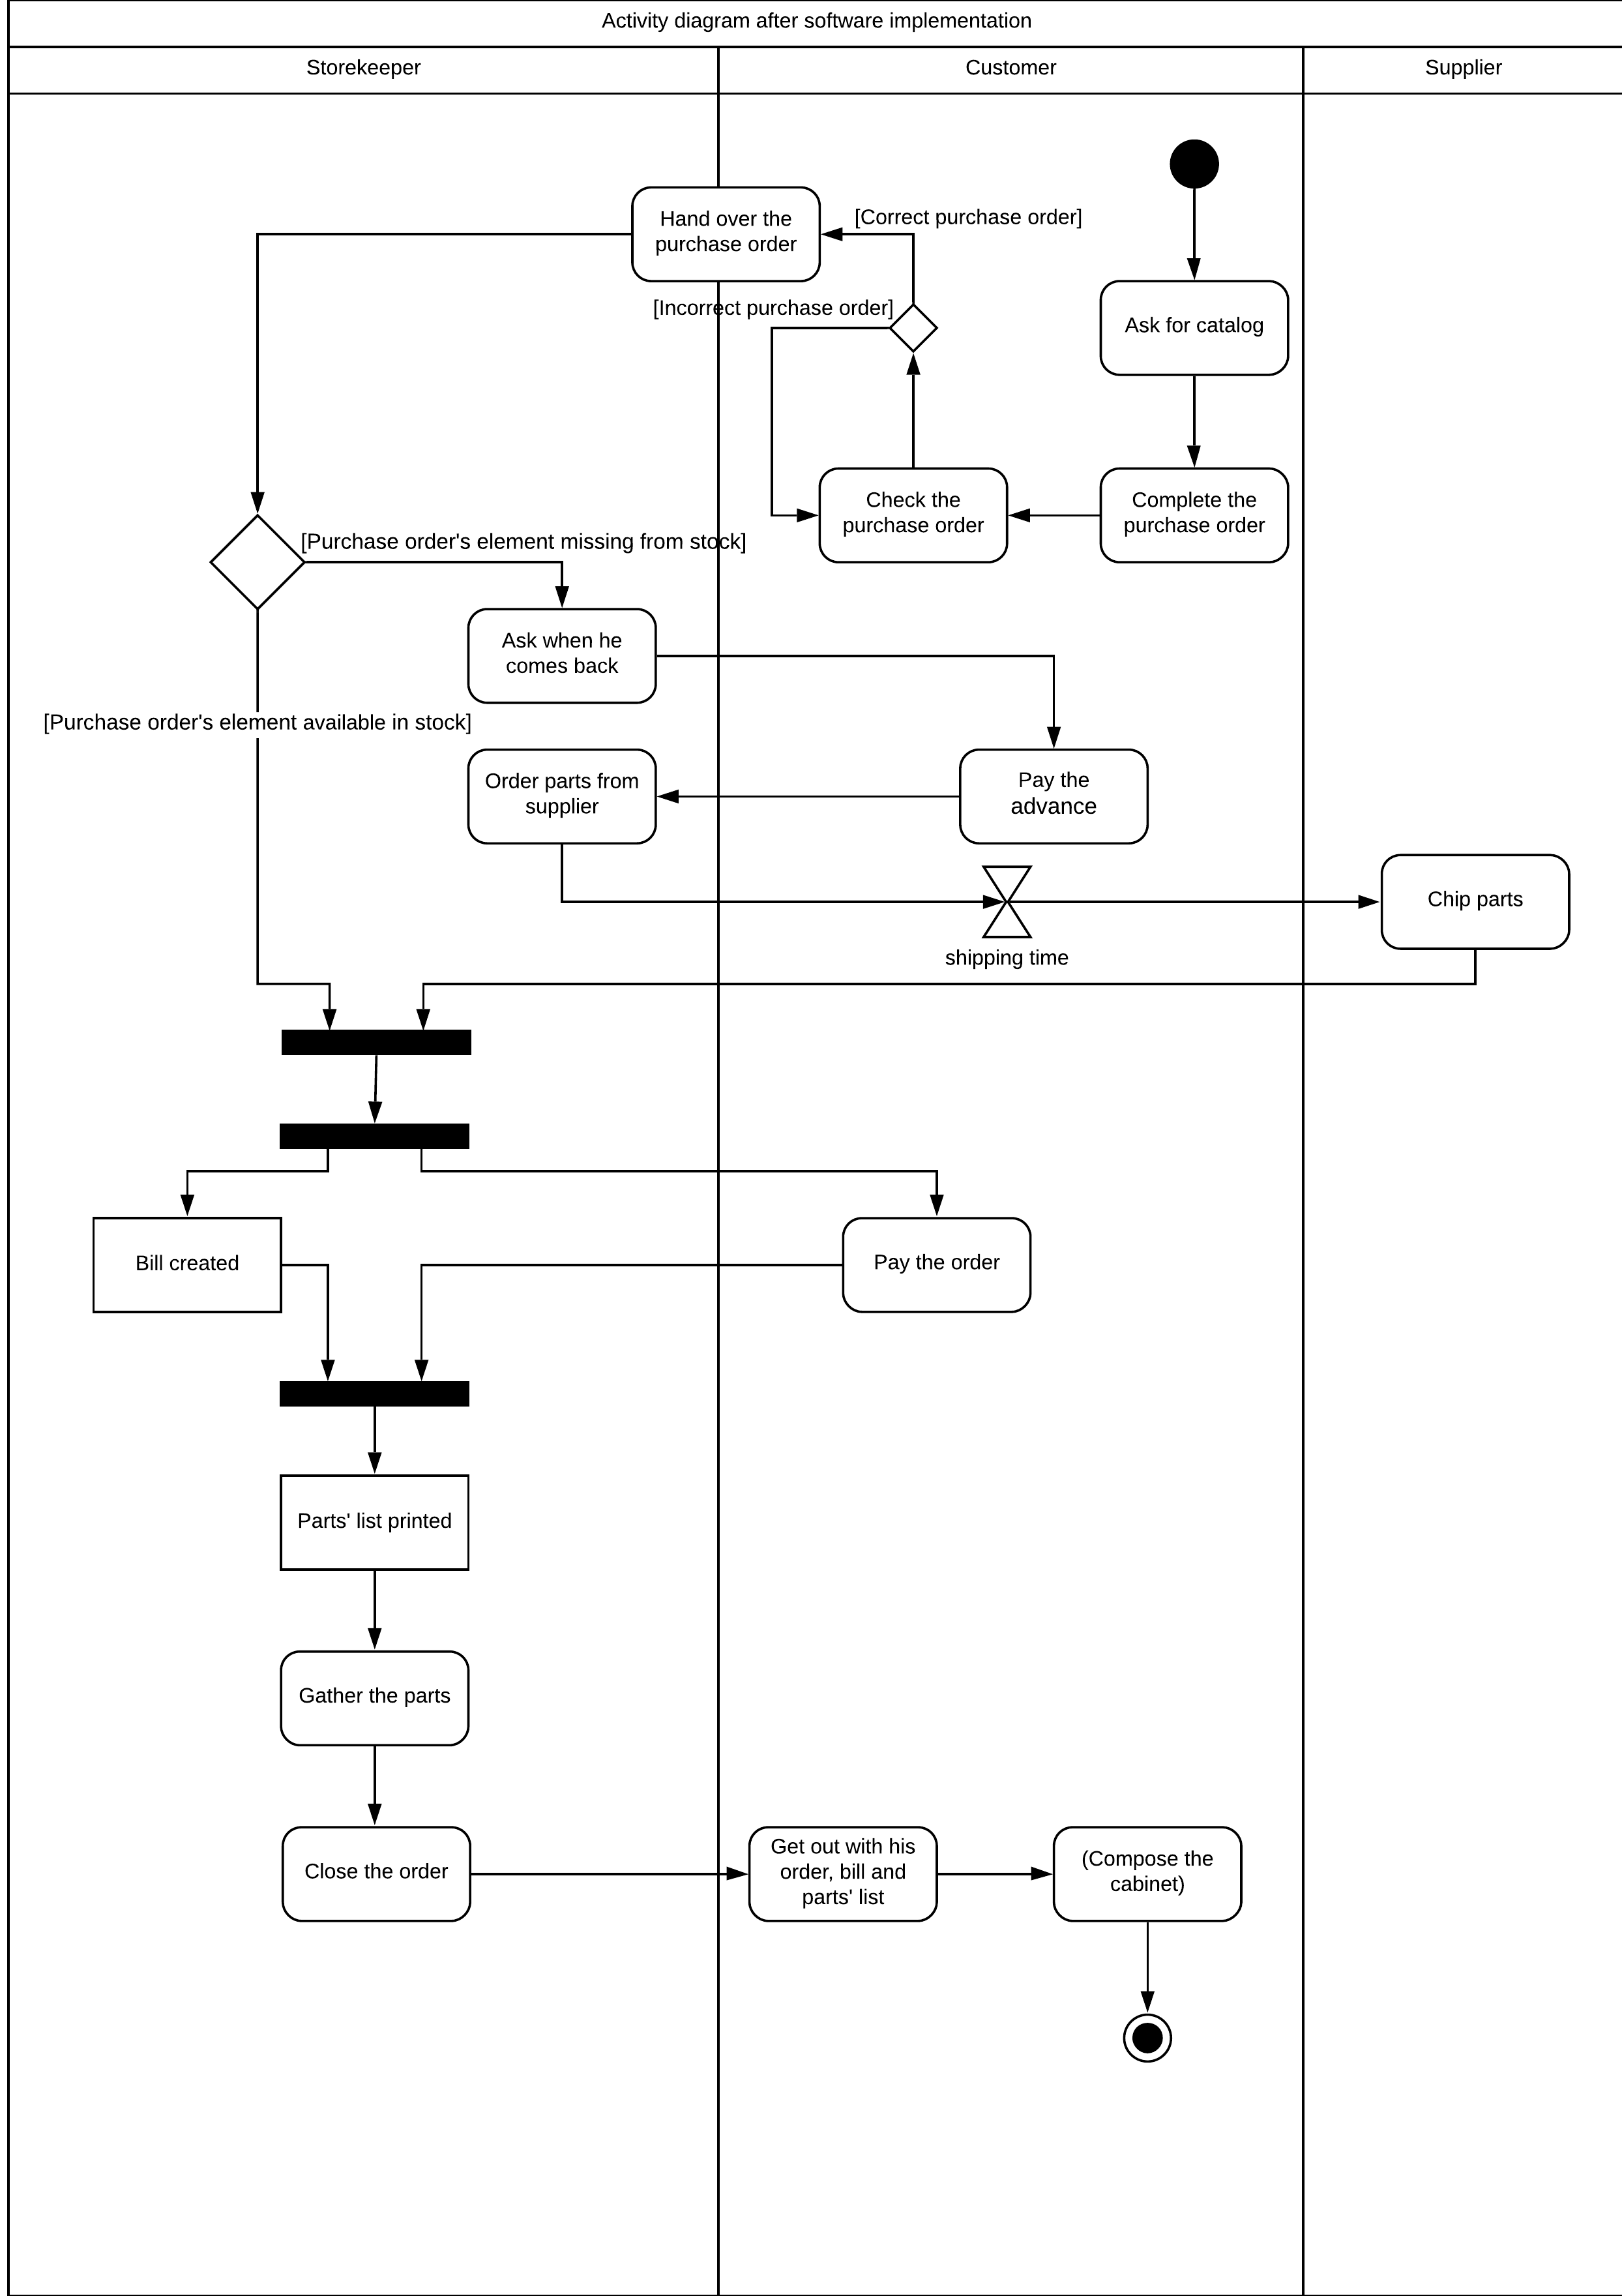
\includegraphics[width =0.8\textwidth]{Figures/ActivityDiagram.png}
			\rule{35em}{0.5pt}
			\caption{Activity Diagram}
			\label{activitydiagram}
    	\end{figure*}
        \vfill
        
    \newpage
    \subsection{Activity Standard Dimension Diagram}
        \vfill
        \begin{figure*}[h!]
            \centering
			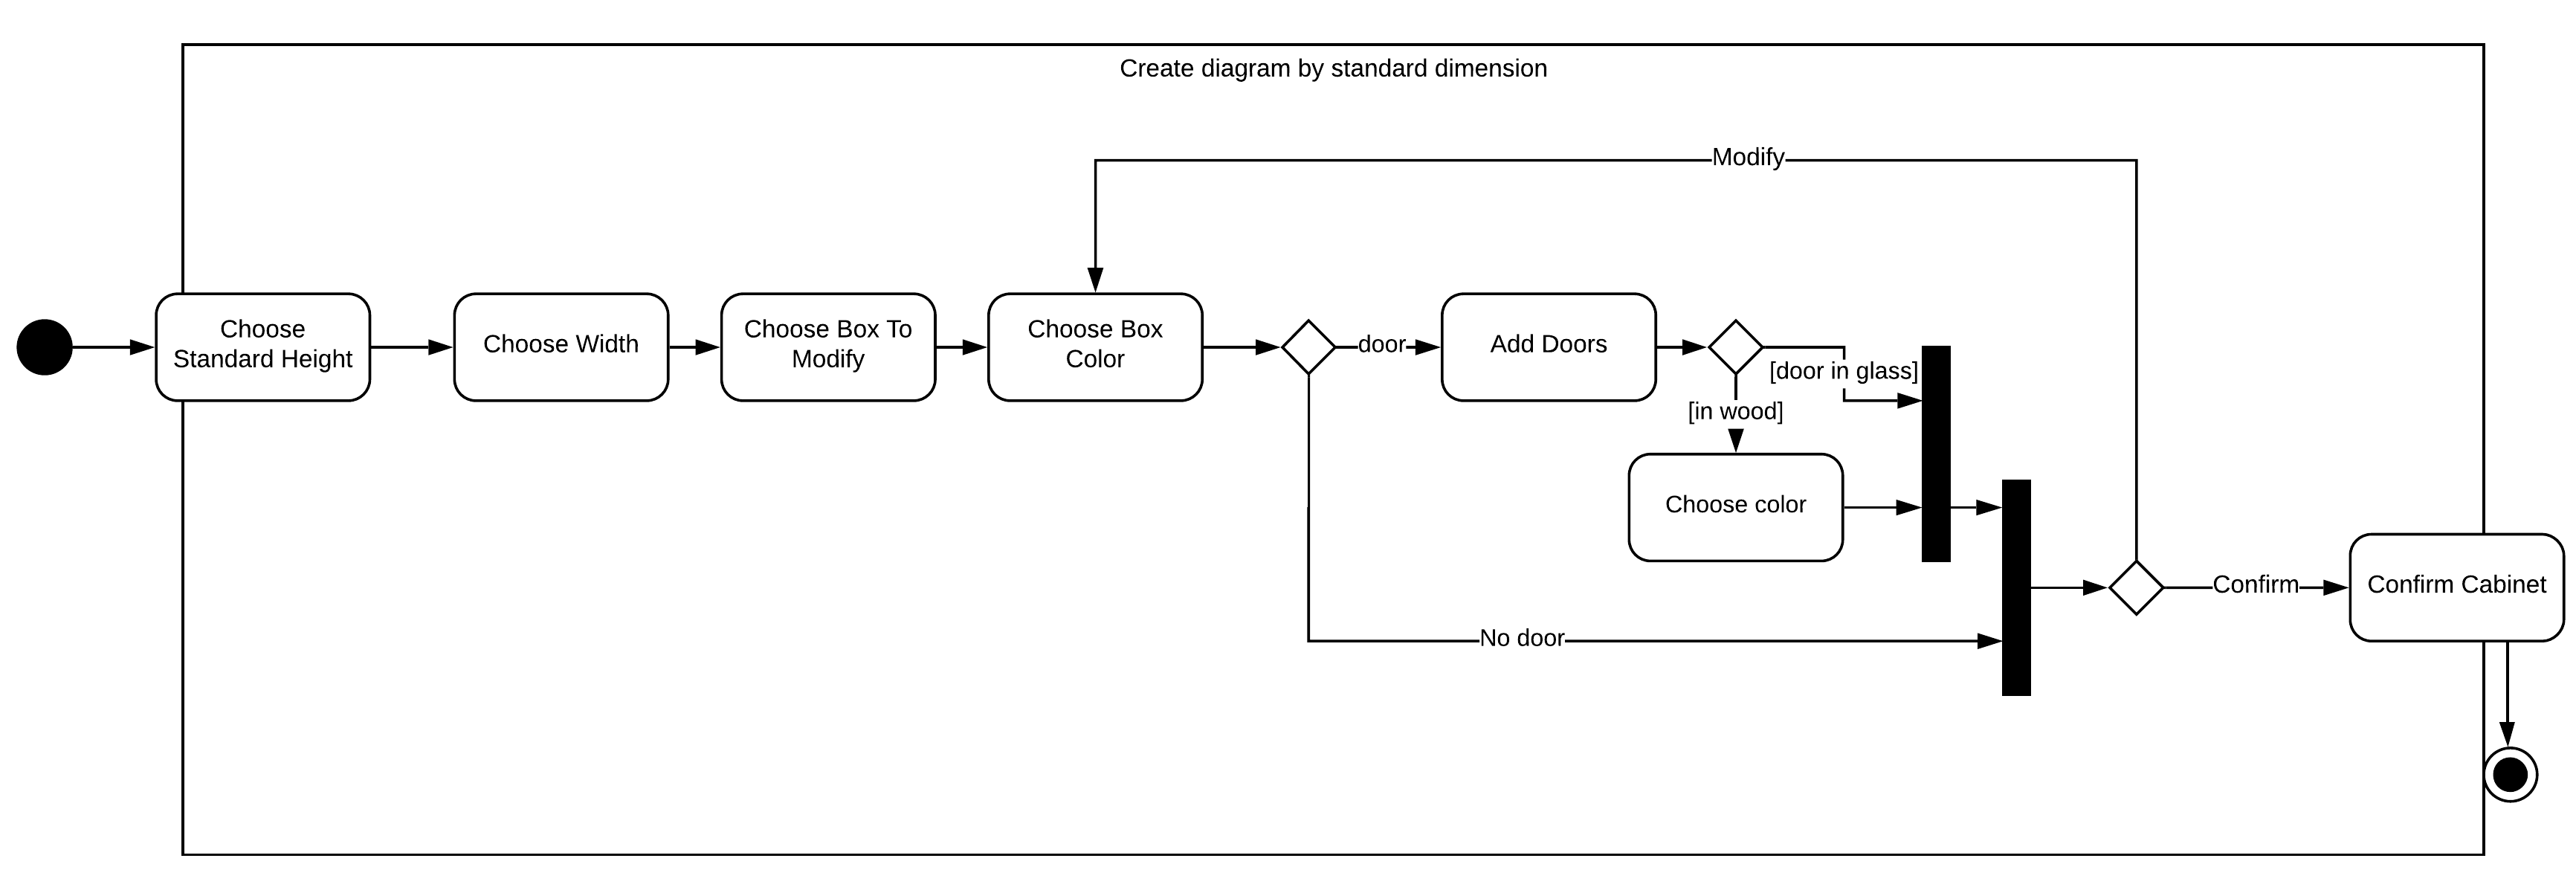
\includegraphics[angle = 90, height=185mm]{Figures/ActivityStandardDiagram.png}
			\rule{35em}{0.5pt}
			\caption{Activity Standard Dimension Diagram}
			\label{activitystandartdiagram}
    	\end{figure*}
        \vfill
        
    \newpage
    \subsection{Activity Cabinet Creation Diagram}
        \vfill
        \begin{figure*}[h!]
            \centering
			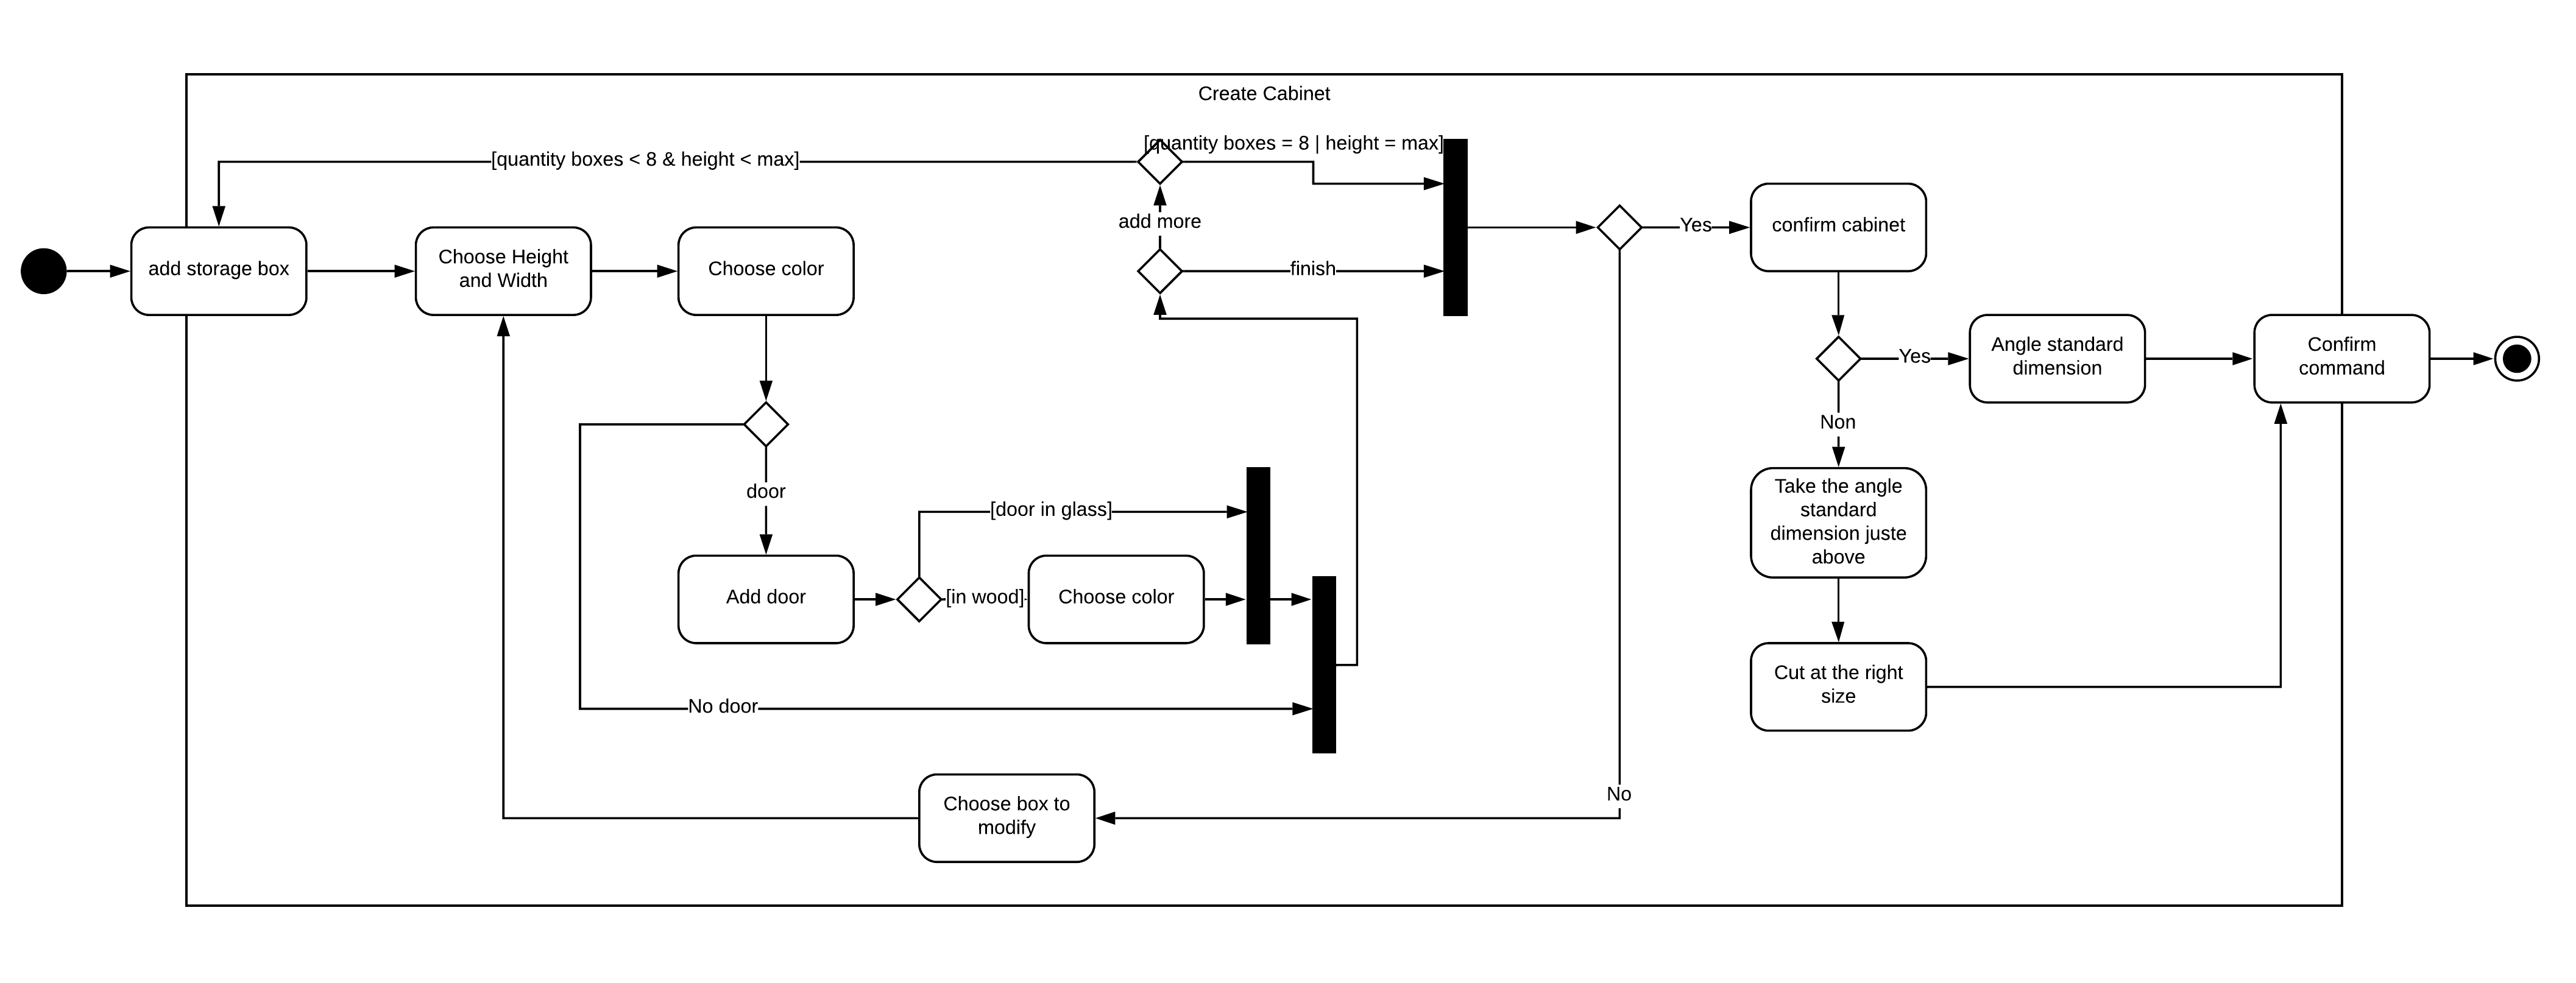
\includegraphics [angle = 90, height=185mm]{Figures/ActivityCabinetDiagram.png}
			\rule{35em}{0.5pt}
			\caption{Activity Cabinet Creation Diagram}
			\label{activitycabinetdiagram}
    	\end{figure*}
        \vfill
        
    \newpage
    \subsection{Use Case Diagram}
        \vfill
        \begin{figure*}[h!]
            \centering
			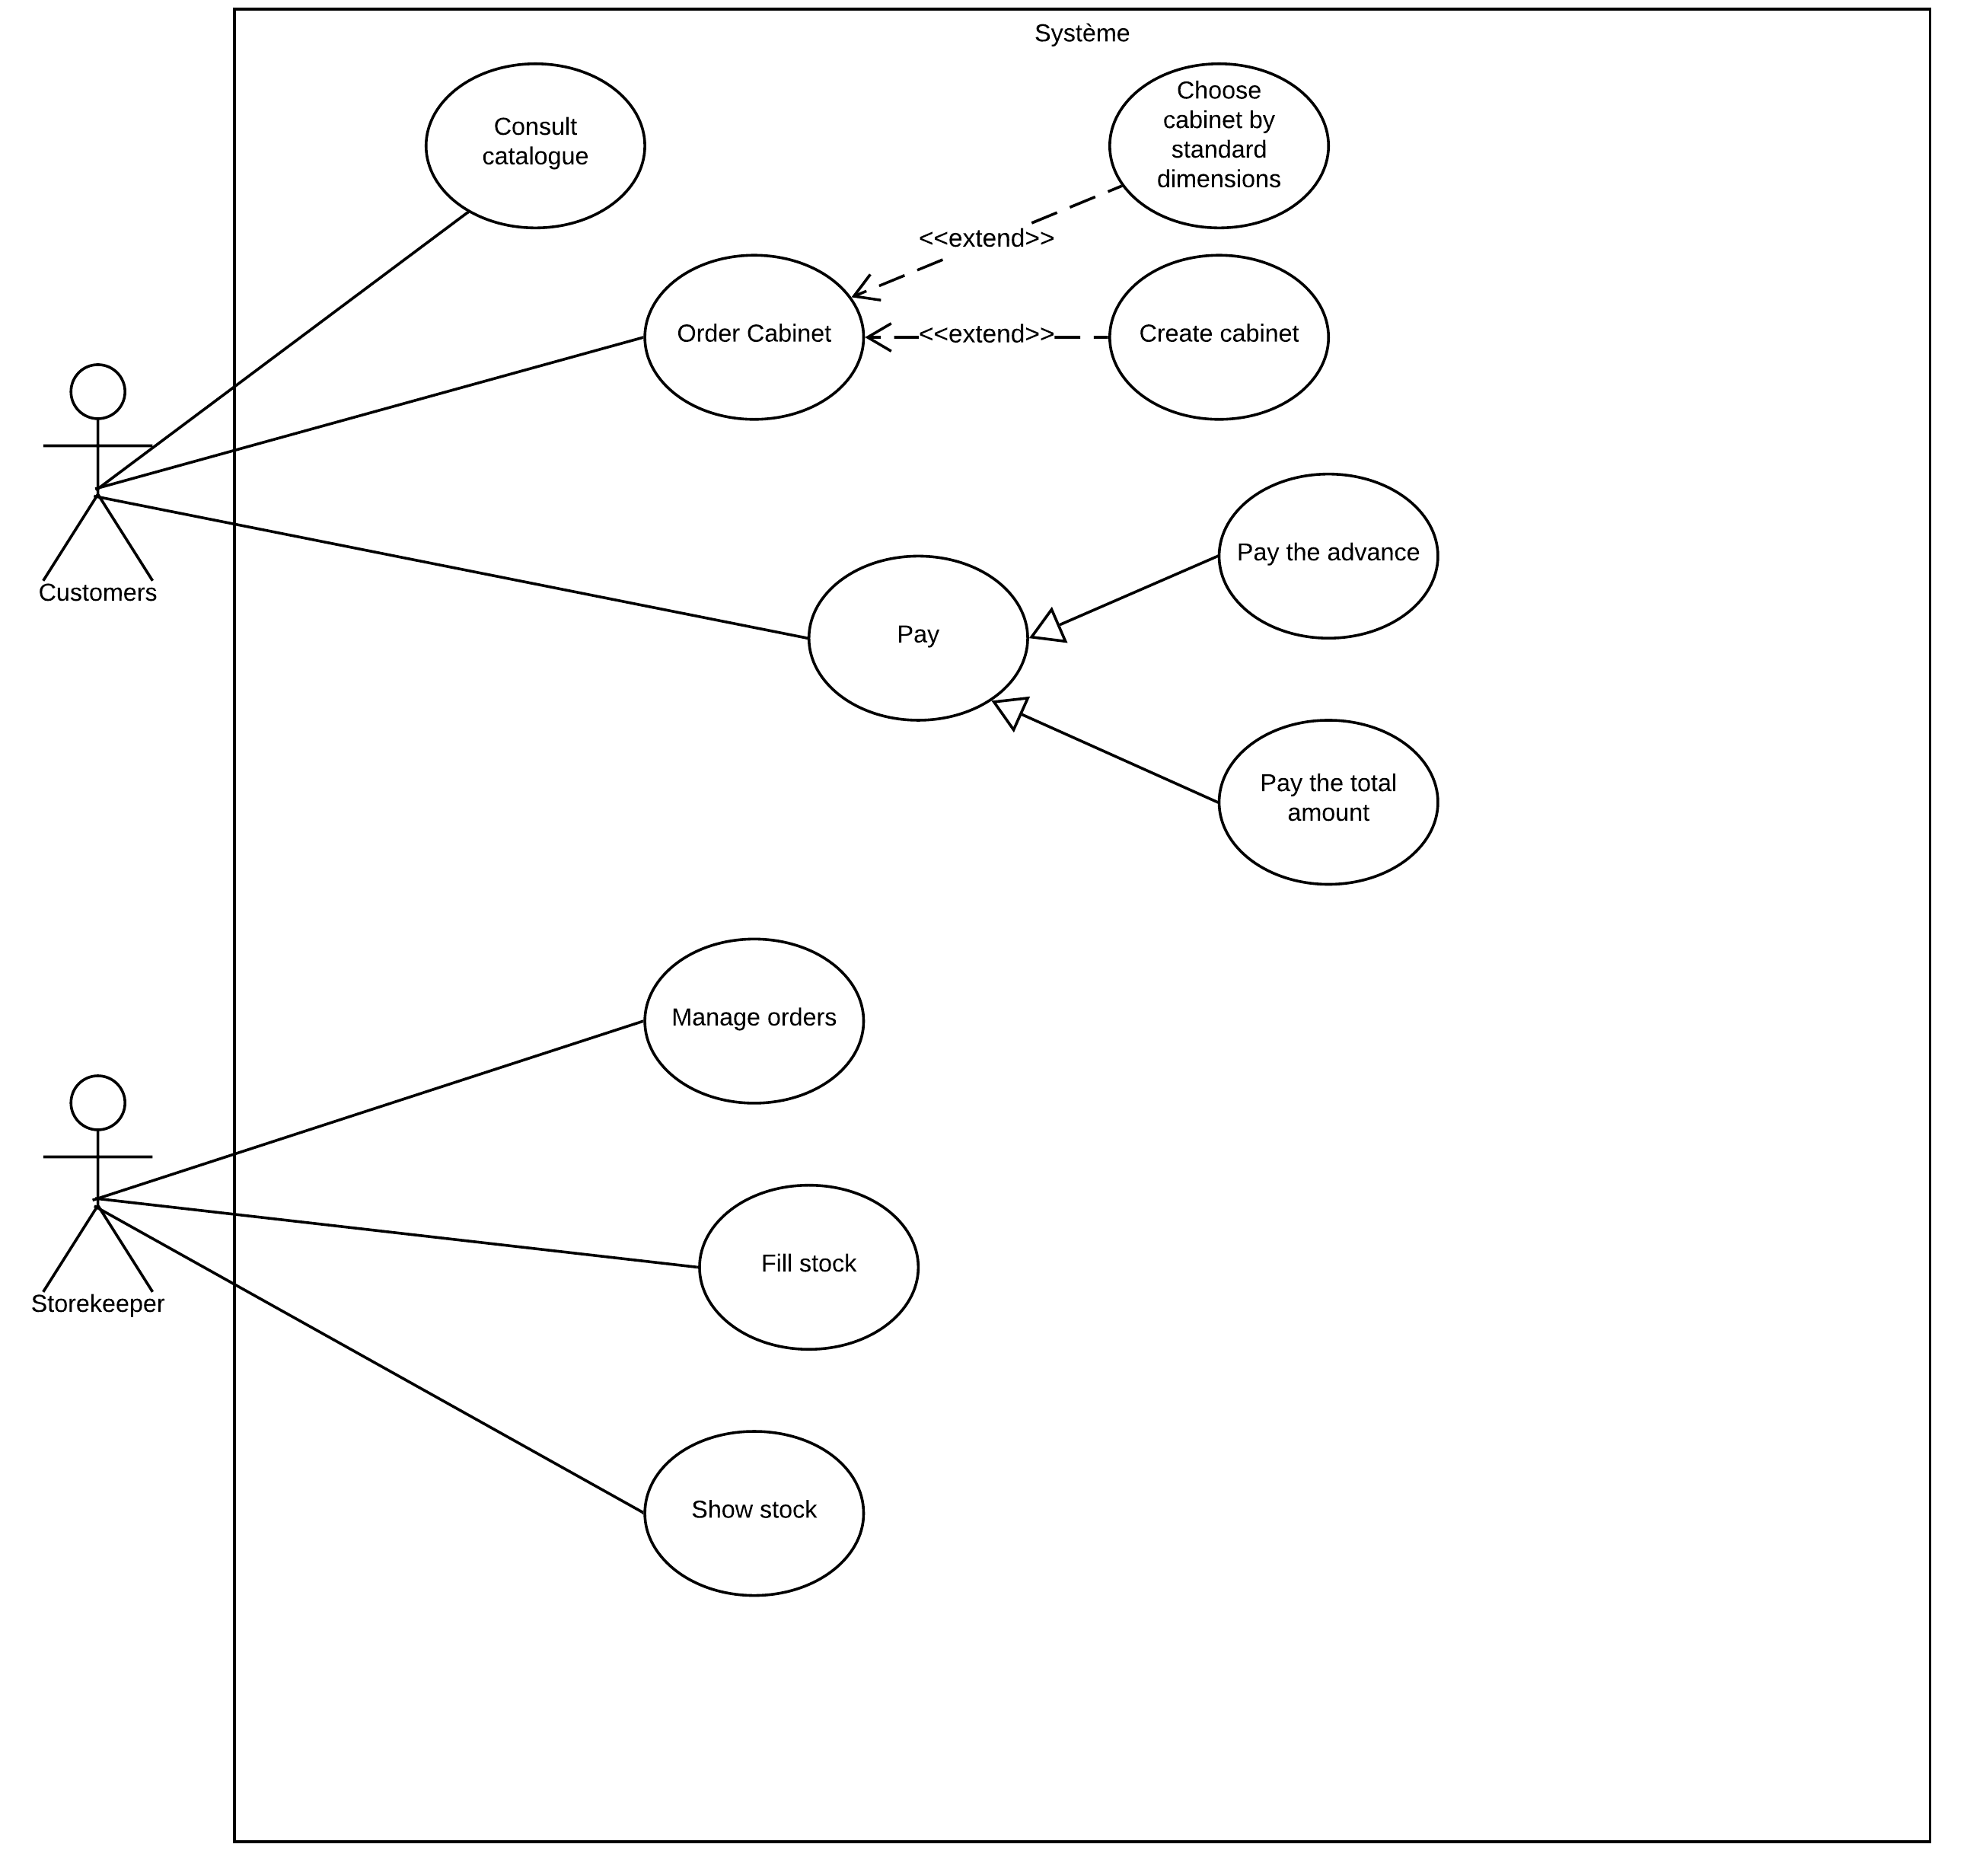
\includegraphics[width =\textwidth]{Figures/UseCaseDiagram.png}
			\rule{35em}{0.5pt}
			\caption{Use Case Diagram}
			\label{usecasediagram}
    	\end{figure*}
        \vfill
        
    \newpage
    \subsection{Class Diagram}
        \begin{figure*}[h!]
            \centering
			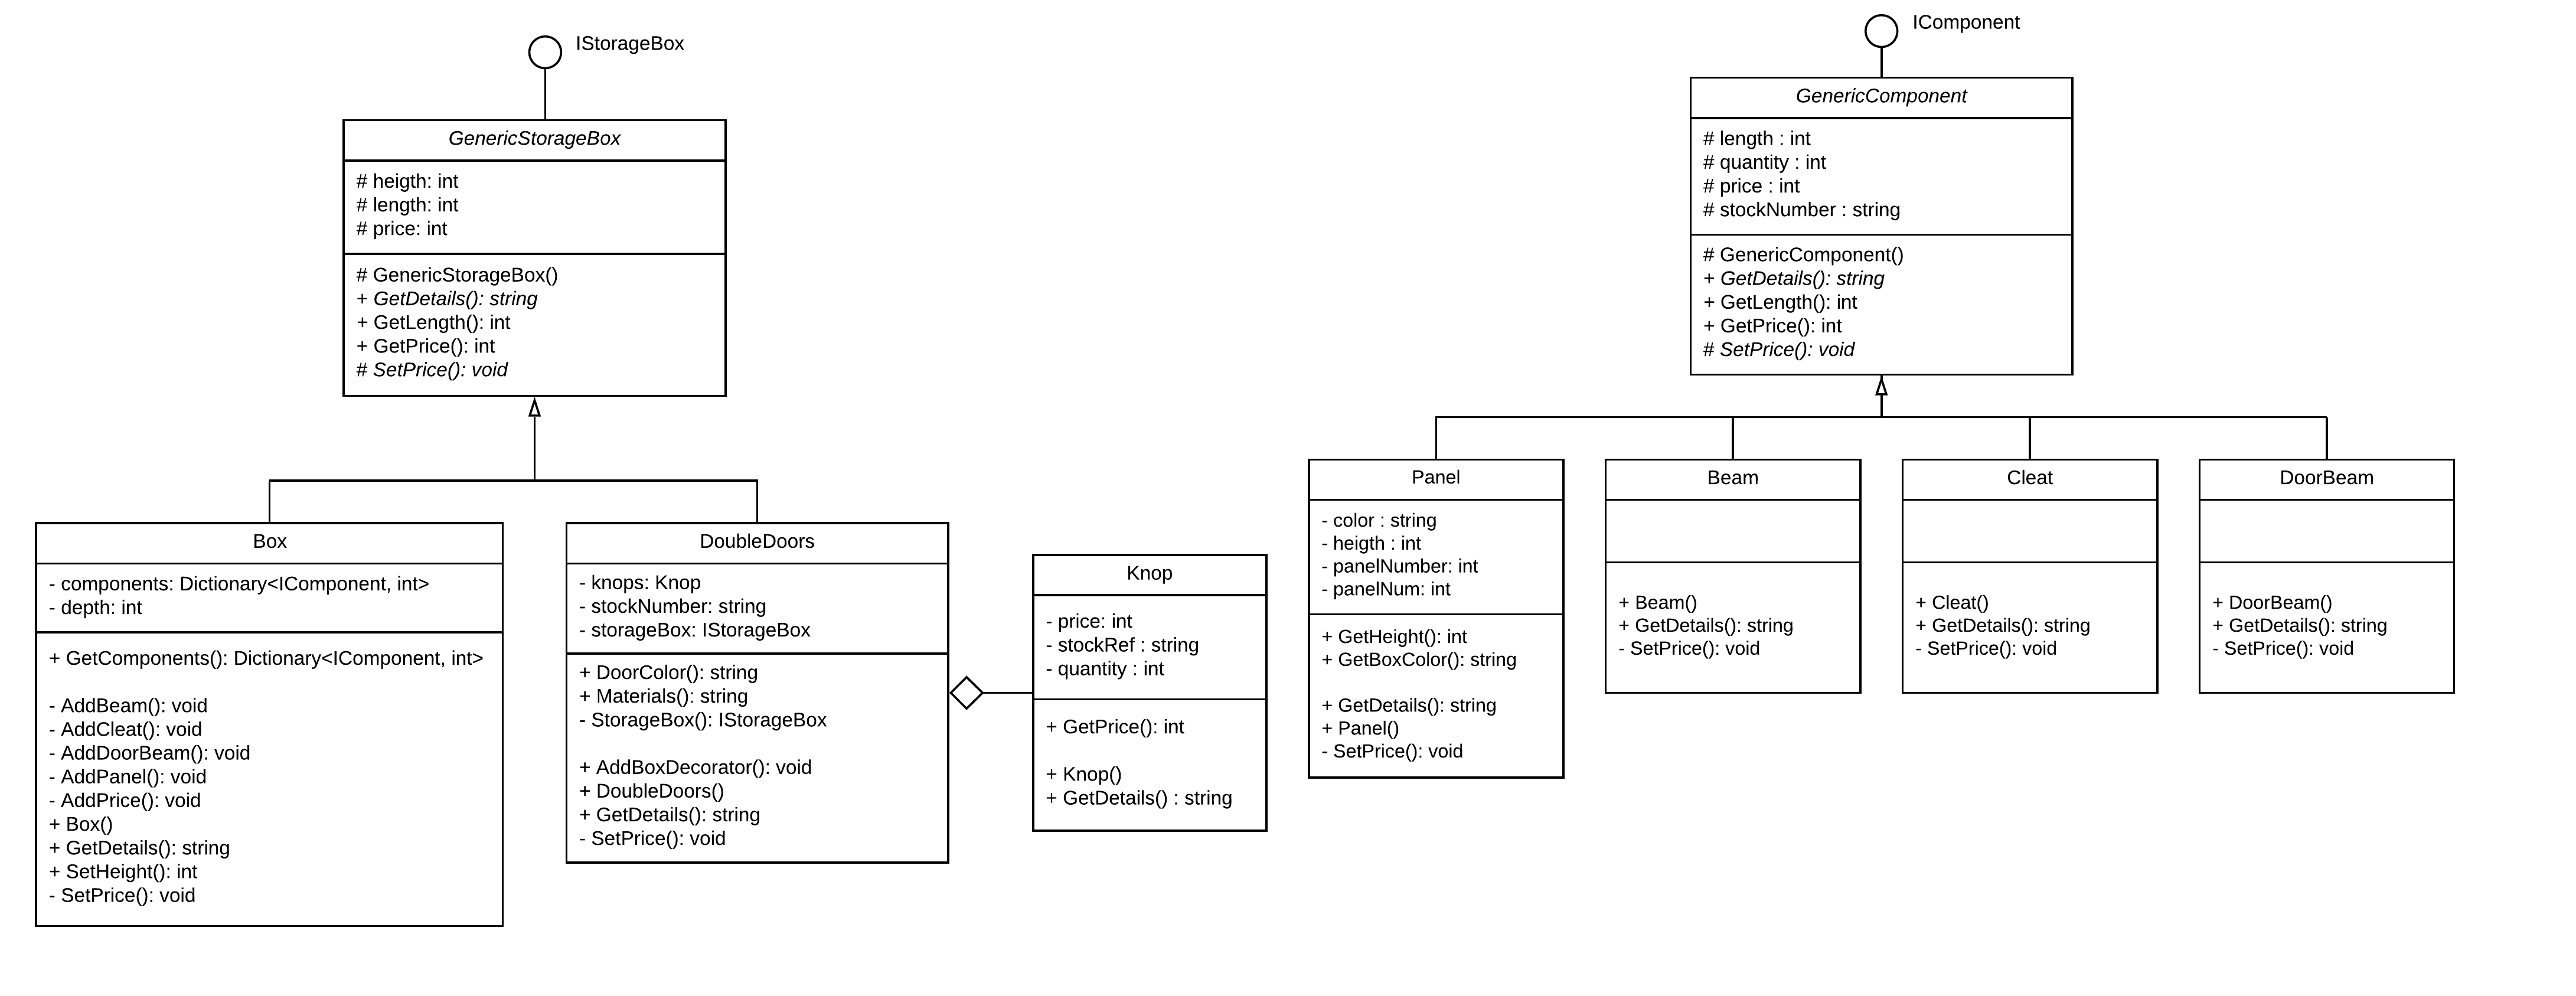
\includegraphics[width = 1.3\textwidth,angle = 90]{Figures/ClassDiagram-1.png}
			\rule{35em}{0.5pt}
			\caption{Class Diagram}
			\label{classdiagram}
    	\end{figure*}
    
    \newpage
    \subsection{Class Diagram – 2}
        \vfill
        \begin{figure*}[h!]
            \centering
			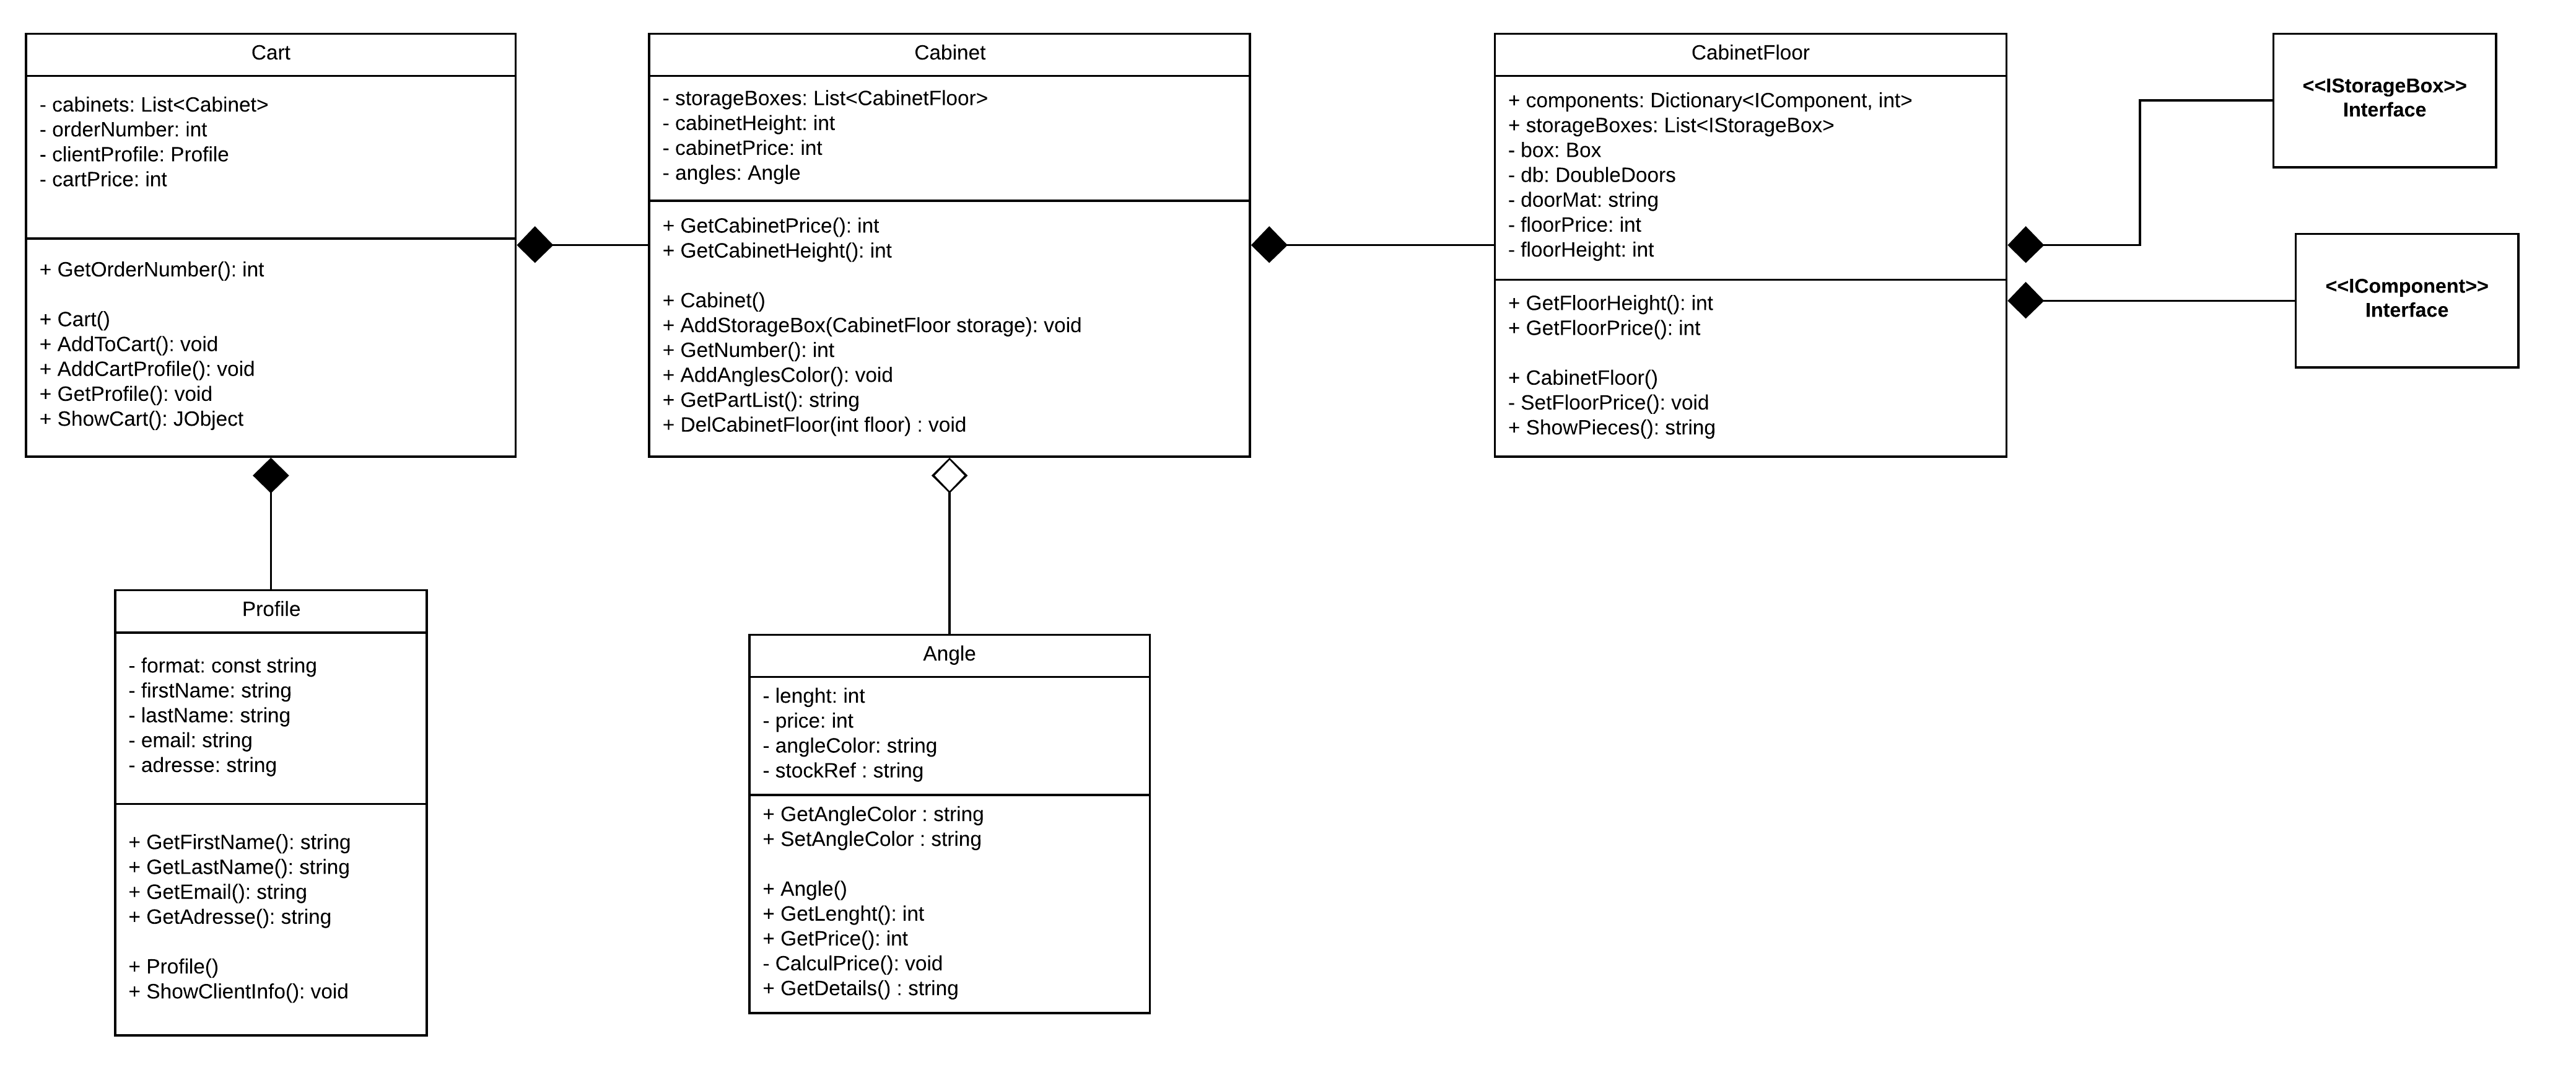
\includegraphics[width = 1.3\textwidth,angle = 90]{Figures/ClassDiagram-2.png}
			\rule{35em}{0.5pt}
			\caption{Class Diagram – 2}
			\label{classdiagram2}
    	\end{figure*}
        \vfill

\newpage
\section{User Interface}
\label{Userinterface}
    \subsection{Homepage}
        \vfill
        \begin{figure*}[h!]
            \centering
    		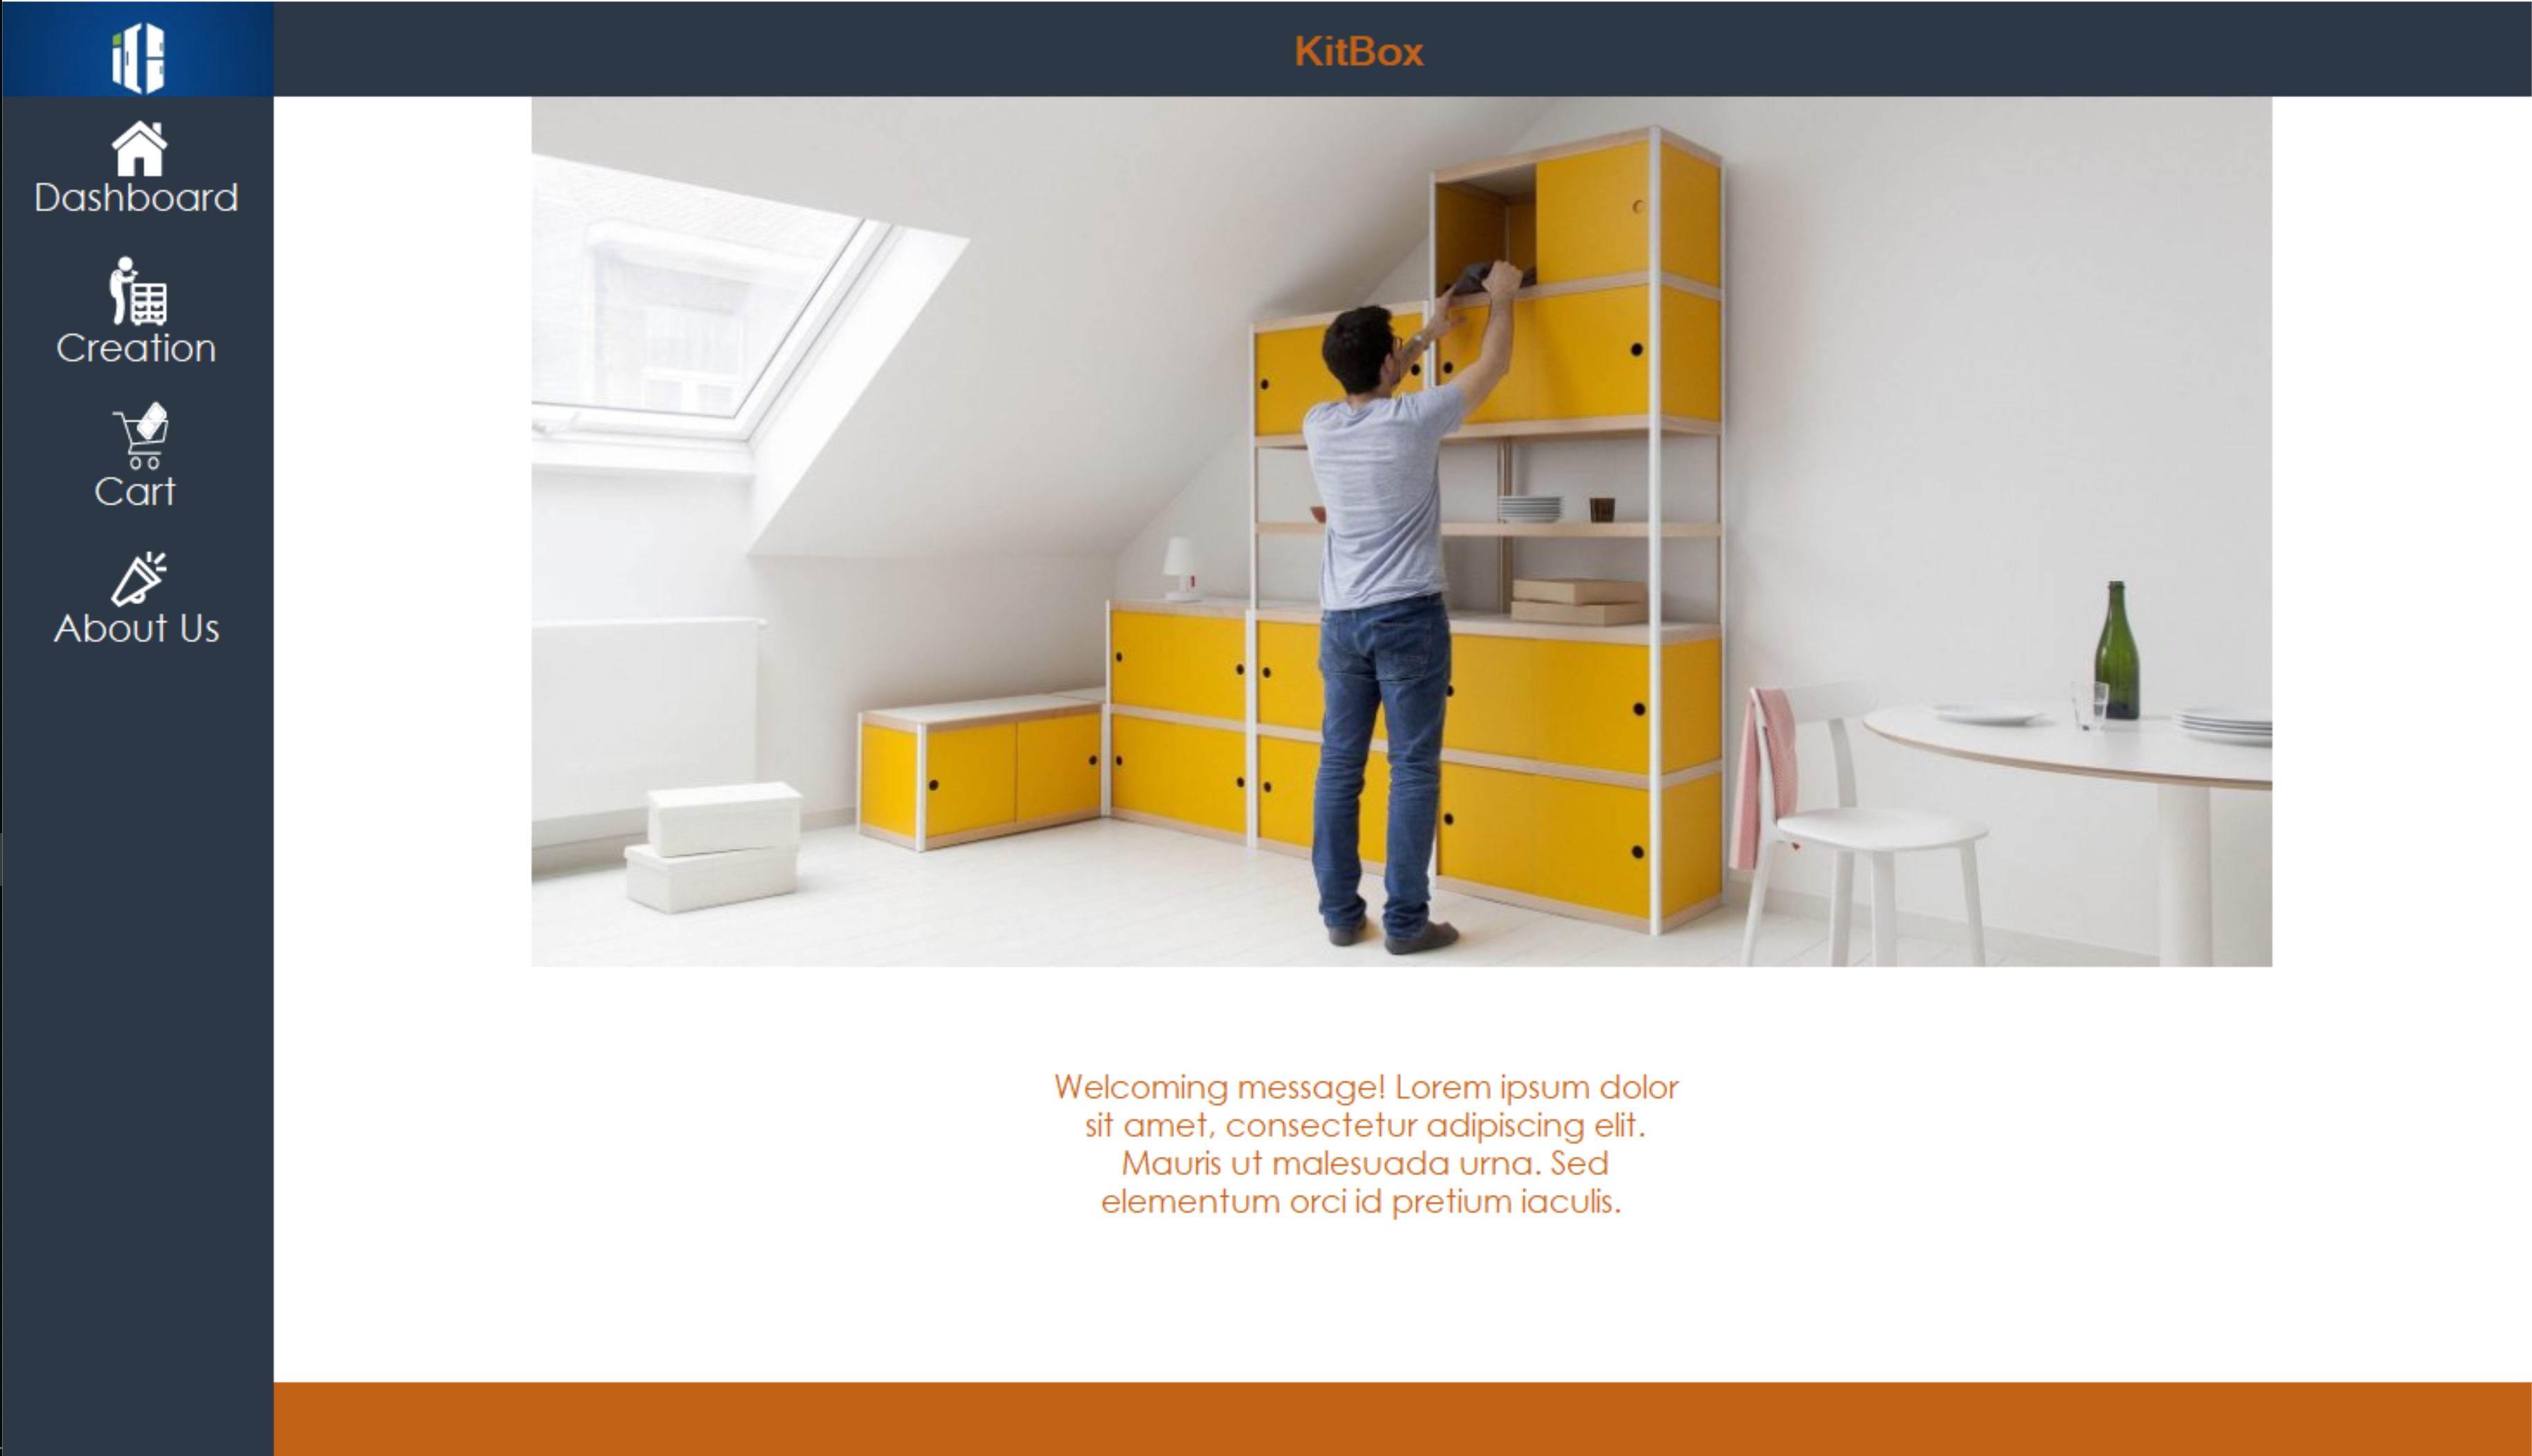
\includegraphics[width =1.2\textwidth,angle = 90]{Figures/Homepage.PNG}
    		\rule{35em}{0.5pt}
    		\caption{Home welcoming page}
    		\label{homepage}
    	\end{figure*}
    	\vfill
    	
	\newpage
	\subsection{Creation welcoming page}
    	\vfill
        \begin{figure*}[h!]
            \centering
    		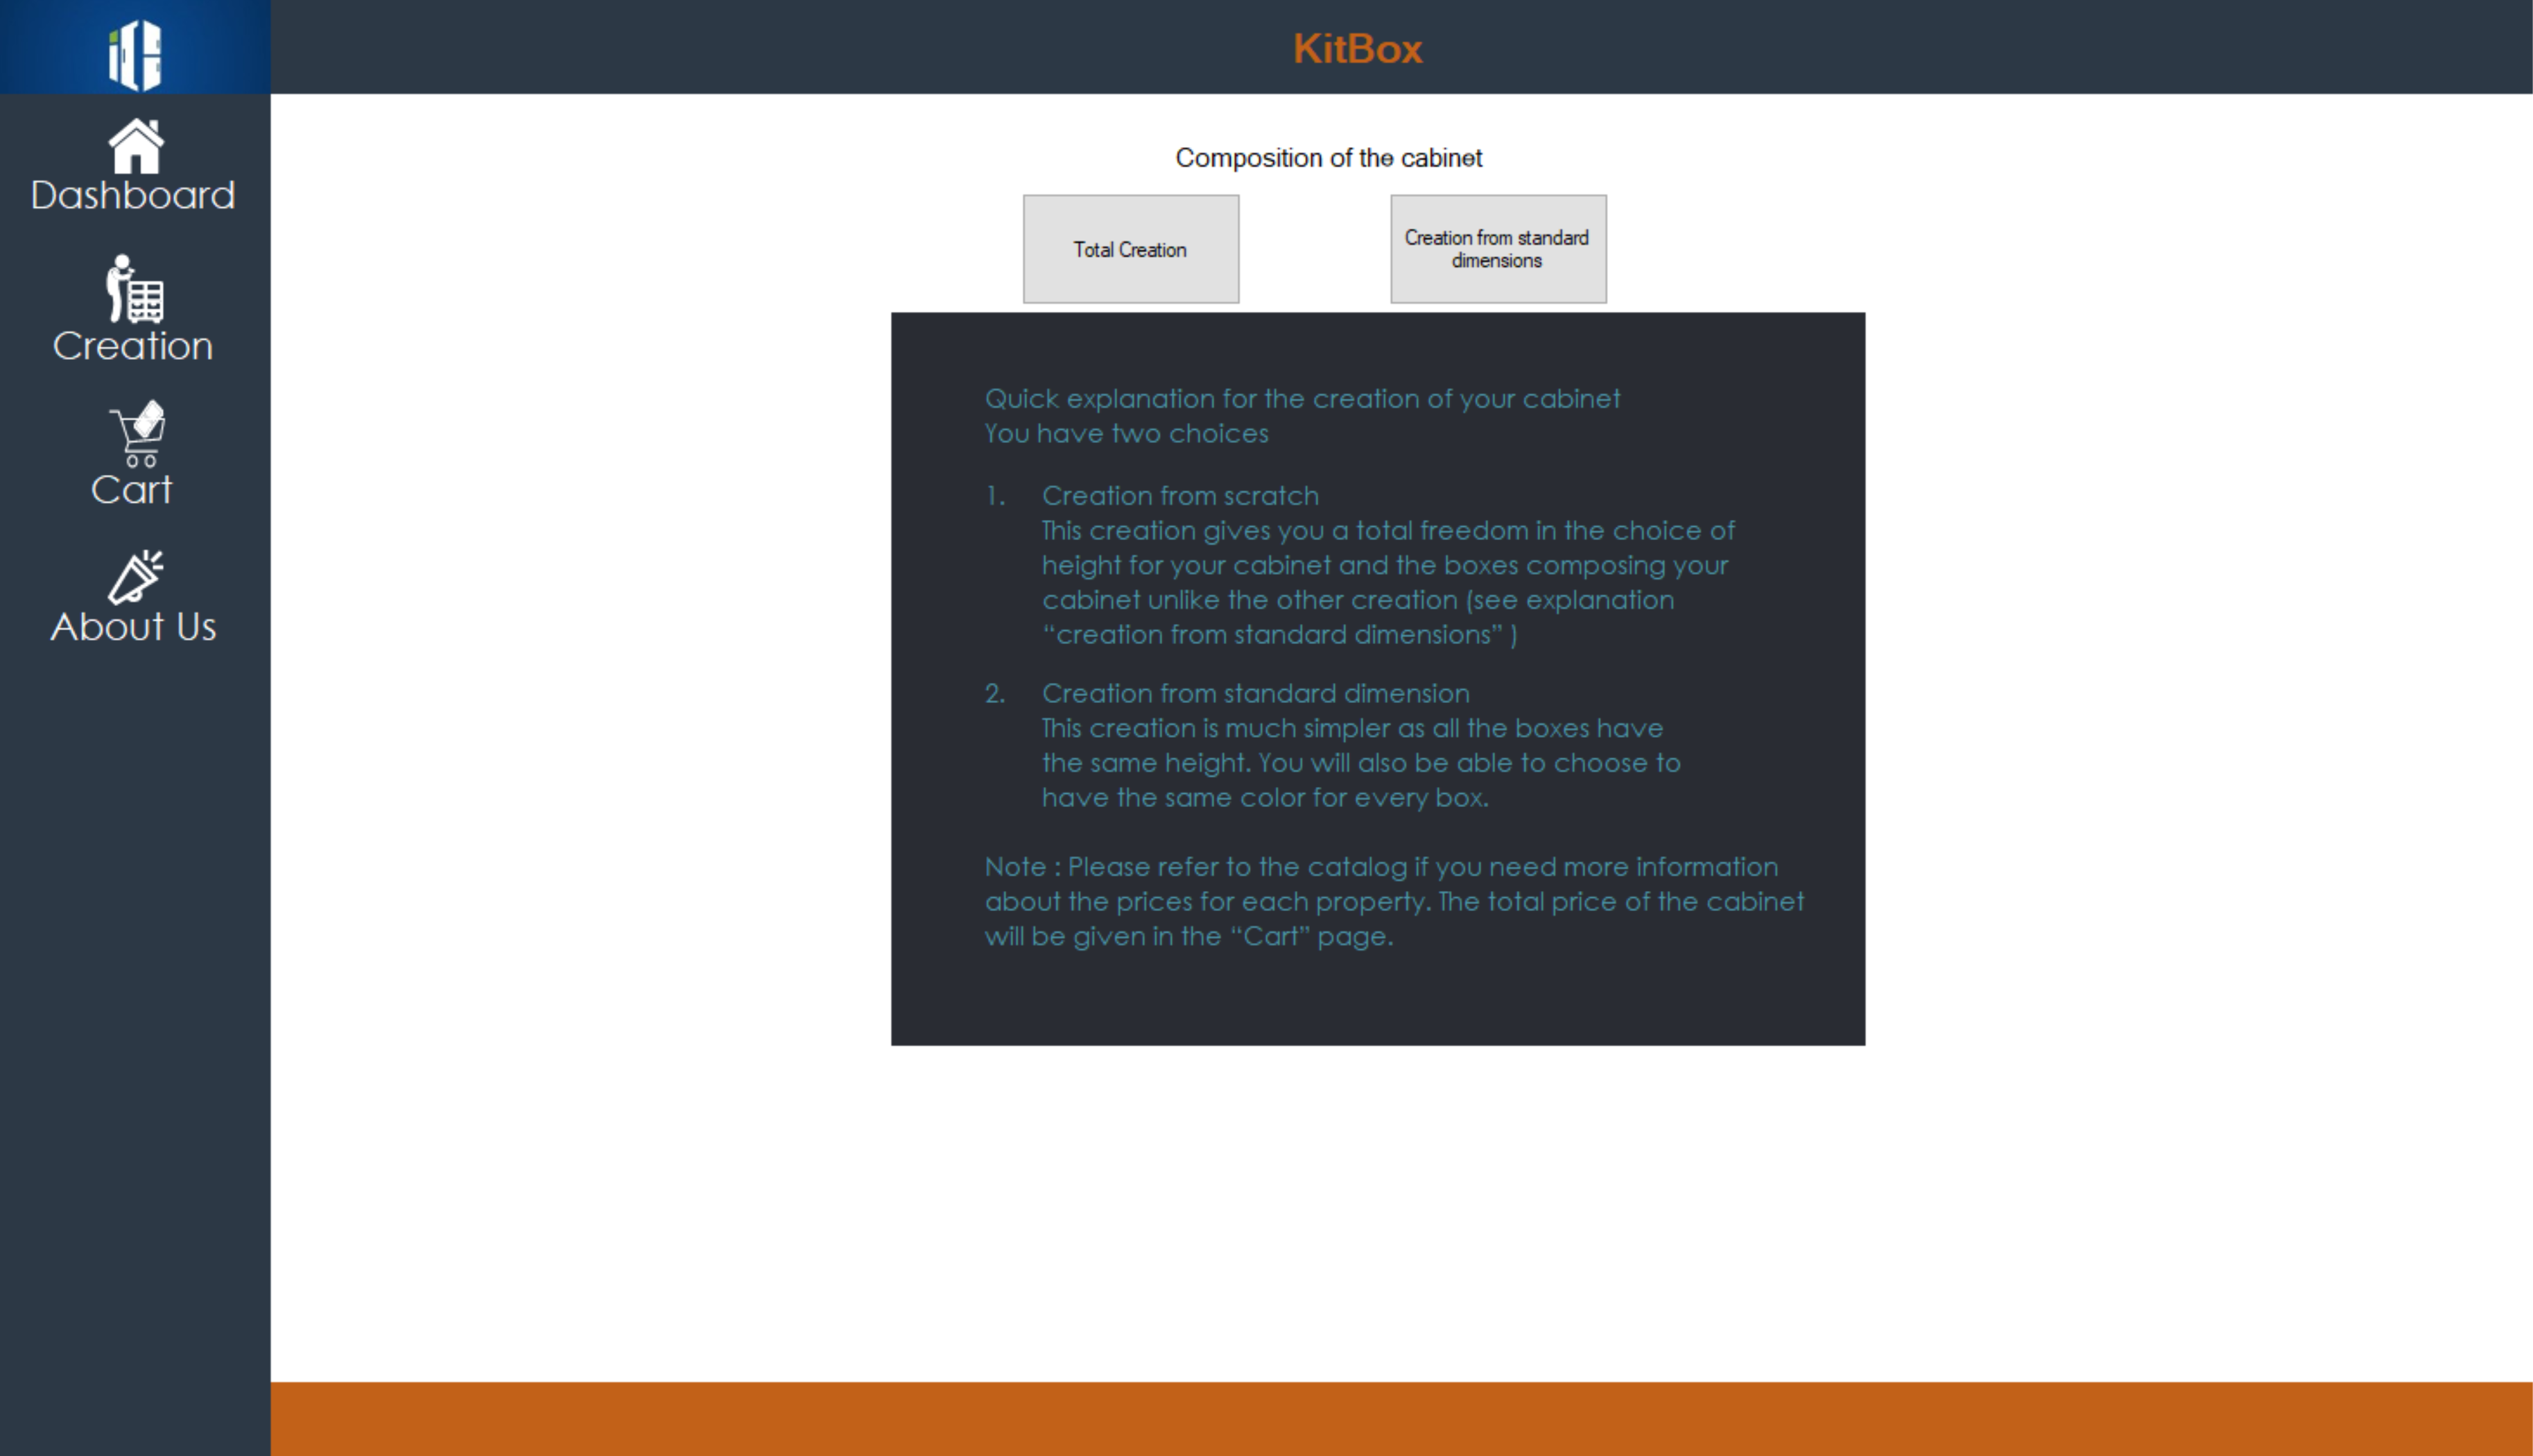
\includegraphics[width =1.2\textwidth,angle = 90]{Figures/creationWelcome.PNG}
    		\rule{35em}{0.5pt}
    		\caption{Creation welcoming page explaining the choices of creation}
    		\label{welcomtab}
    	\end{figure*}
    	\vfill
    	
	\newpage
	\subsection{Creation from Scratch}
    	\vfill
        \begin{figure*}[h!]
            \centering
    		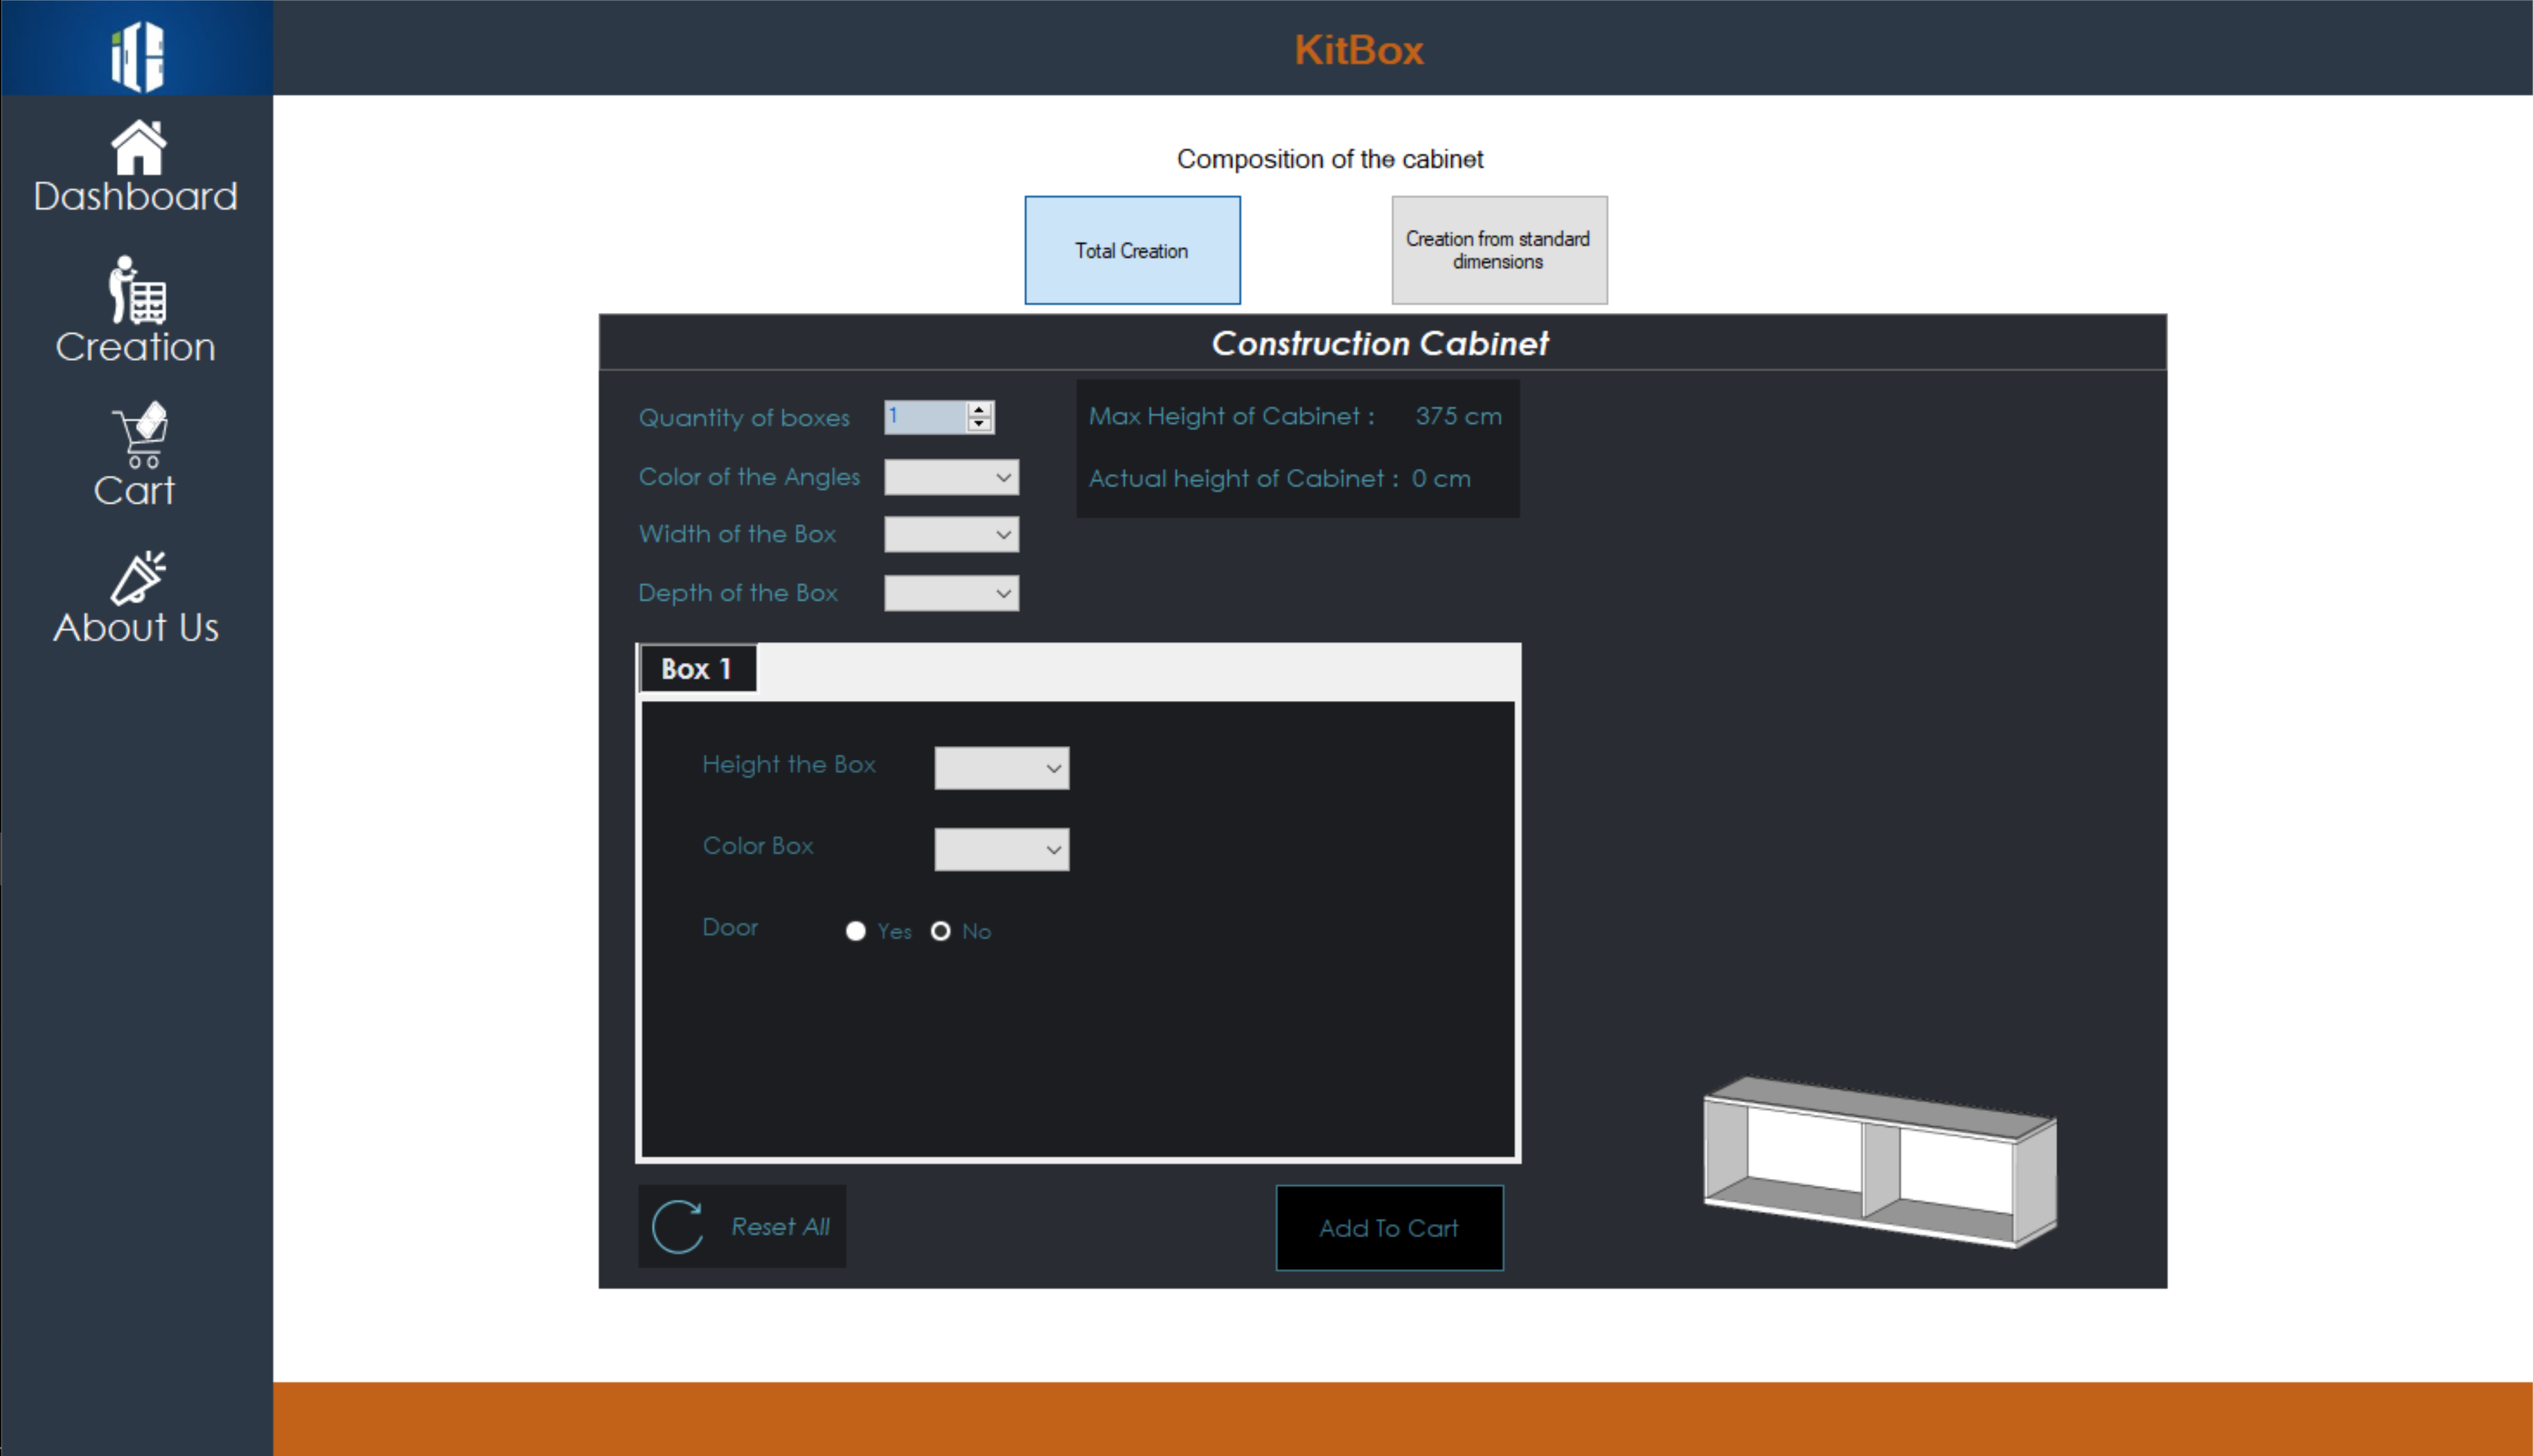
\includegraphics[width =1.2\textwidth,angle = 90]{Figures/CreationScratch.PNG}
    		\rule{35em}{0.5pt}
    		\caption{Creation from Scratch initial state}
    		\label{ordertab}
    	\end{figure*}
    	\vfill
    	
	\newpage
	\subsection{Creation from Scratch filled}
    	\vfill
        \begin{figure*}[h!]
            \centering
    		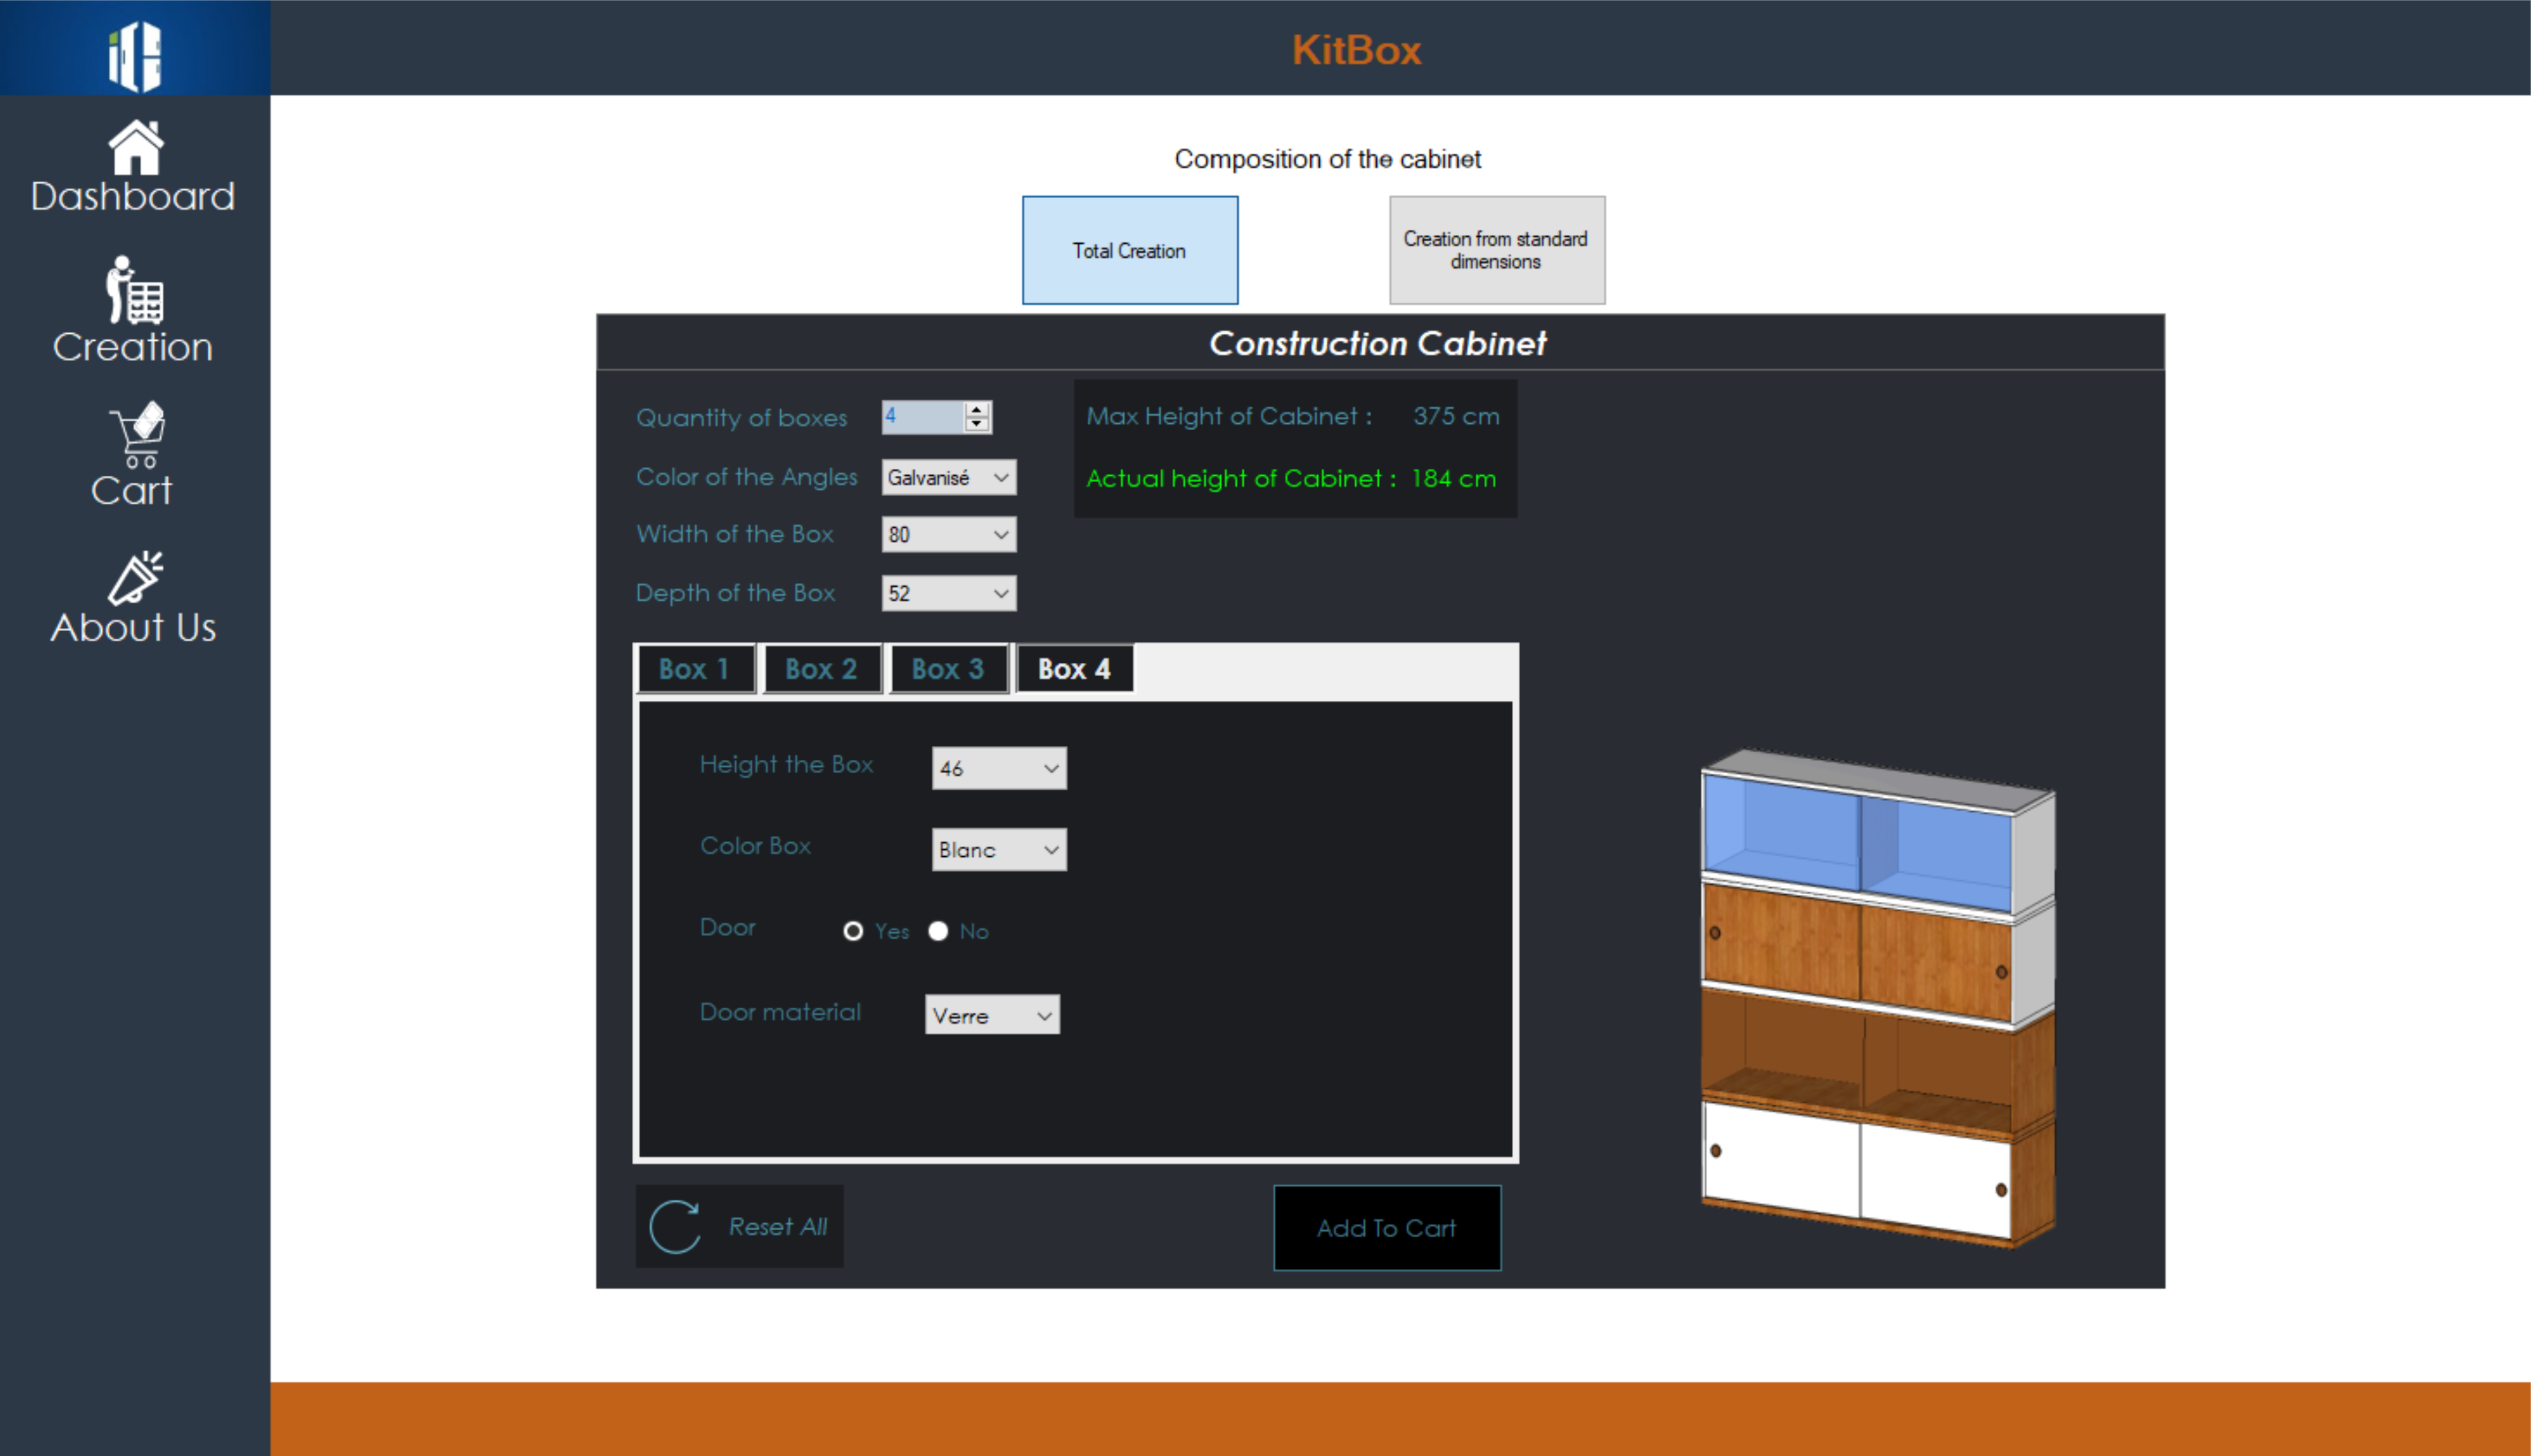
\includegraphics[width =1.2\textwidth,angle = 90]{Figures/CreationScratchFilled.PNG}
    		\rule{35em}{0.5pt}
    		\caption{Creation from Scratch after filling all the features}
    		\label{scratchtab}
    	\end{figure*}
    	\vfill
    	
	\newpage
	\subsection{Creation from standard dimensions}
    	\vfill
        \begin{figure*}[h!]
            \centering
    		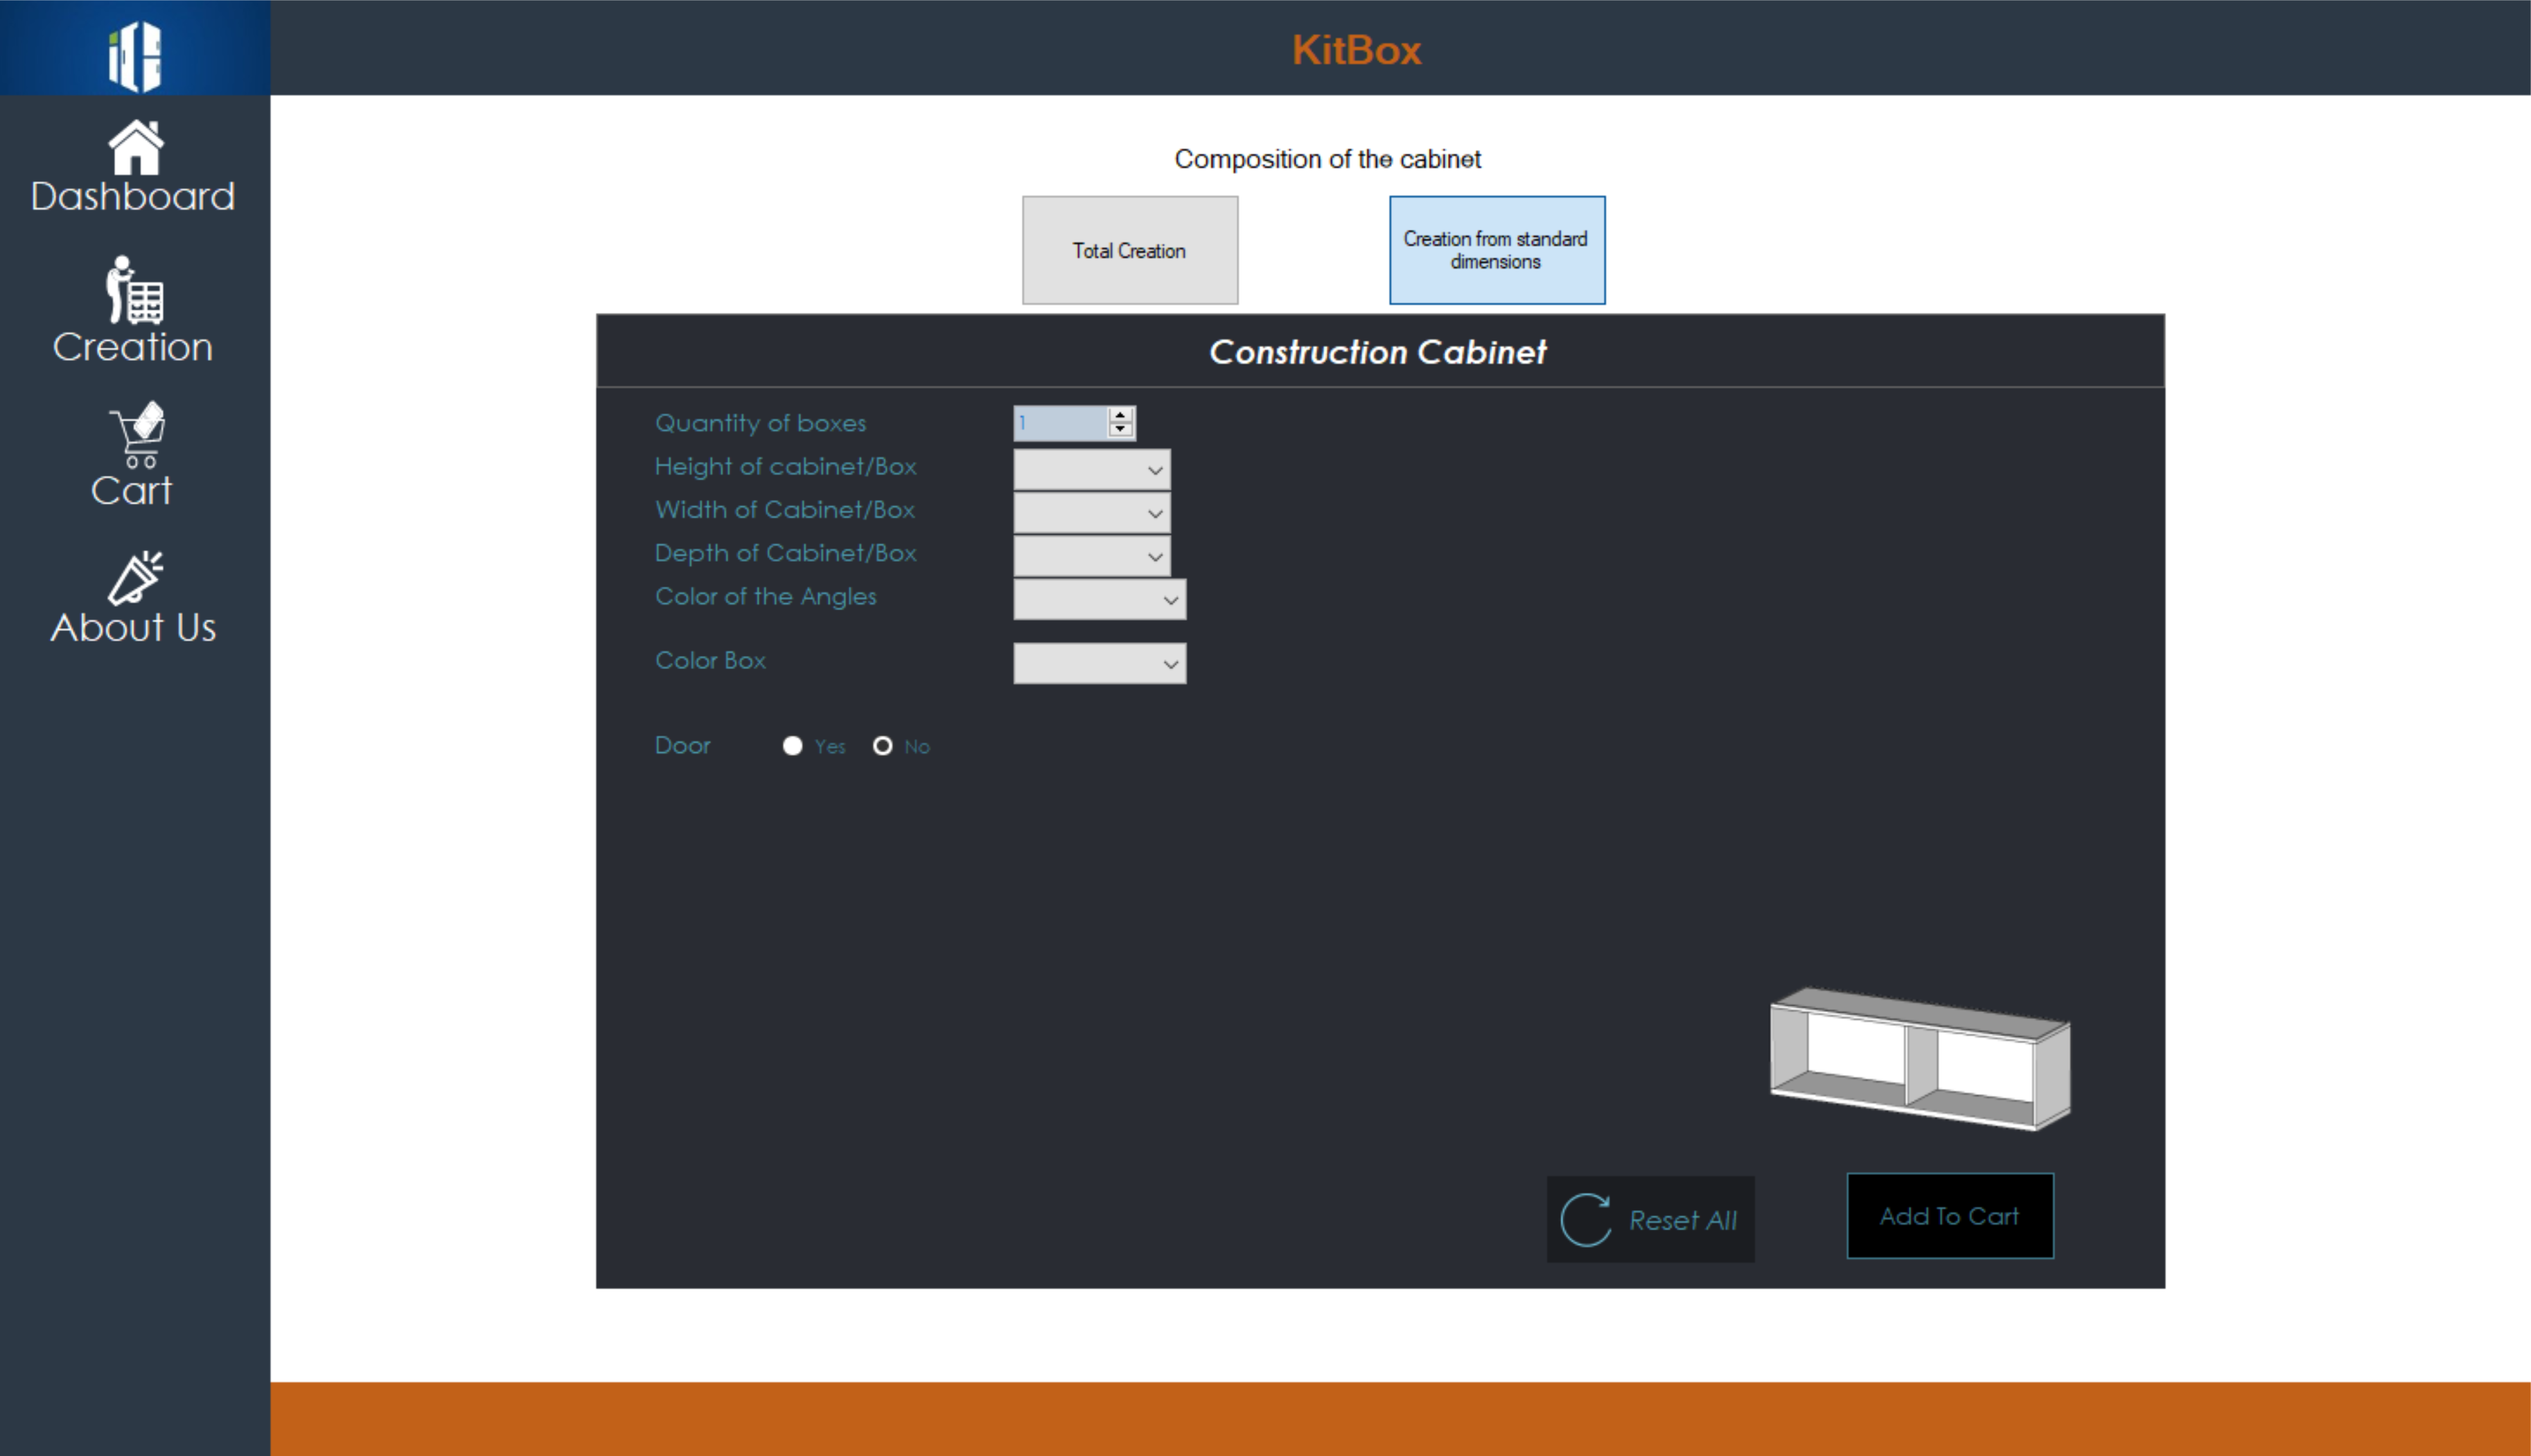
\includegraphics[height=110truemm,angle = 90]{Figures/CreationStandard.PNG}
    		\rule{35em}{0.5pt}
    		\caption{Creation from standard dimensions initial state}
    		\label{standardtab}
    	\end{figure*}
    	\vfill
    	
	\newpage
	\subsection{Creation from standard dimensions filled}
    	\vfill
        \begin{figure*}[h!]
            \centering
    		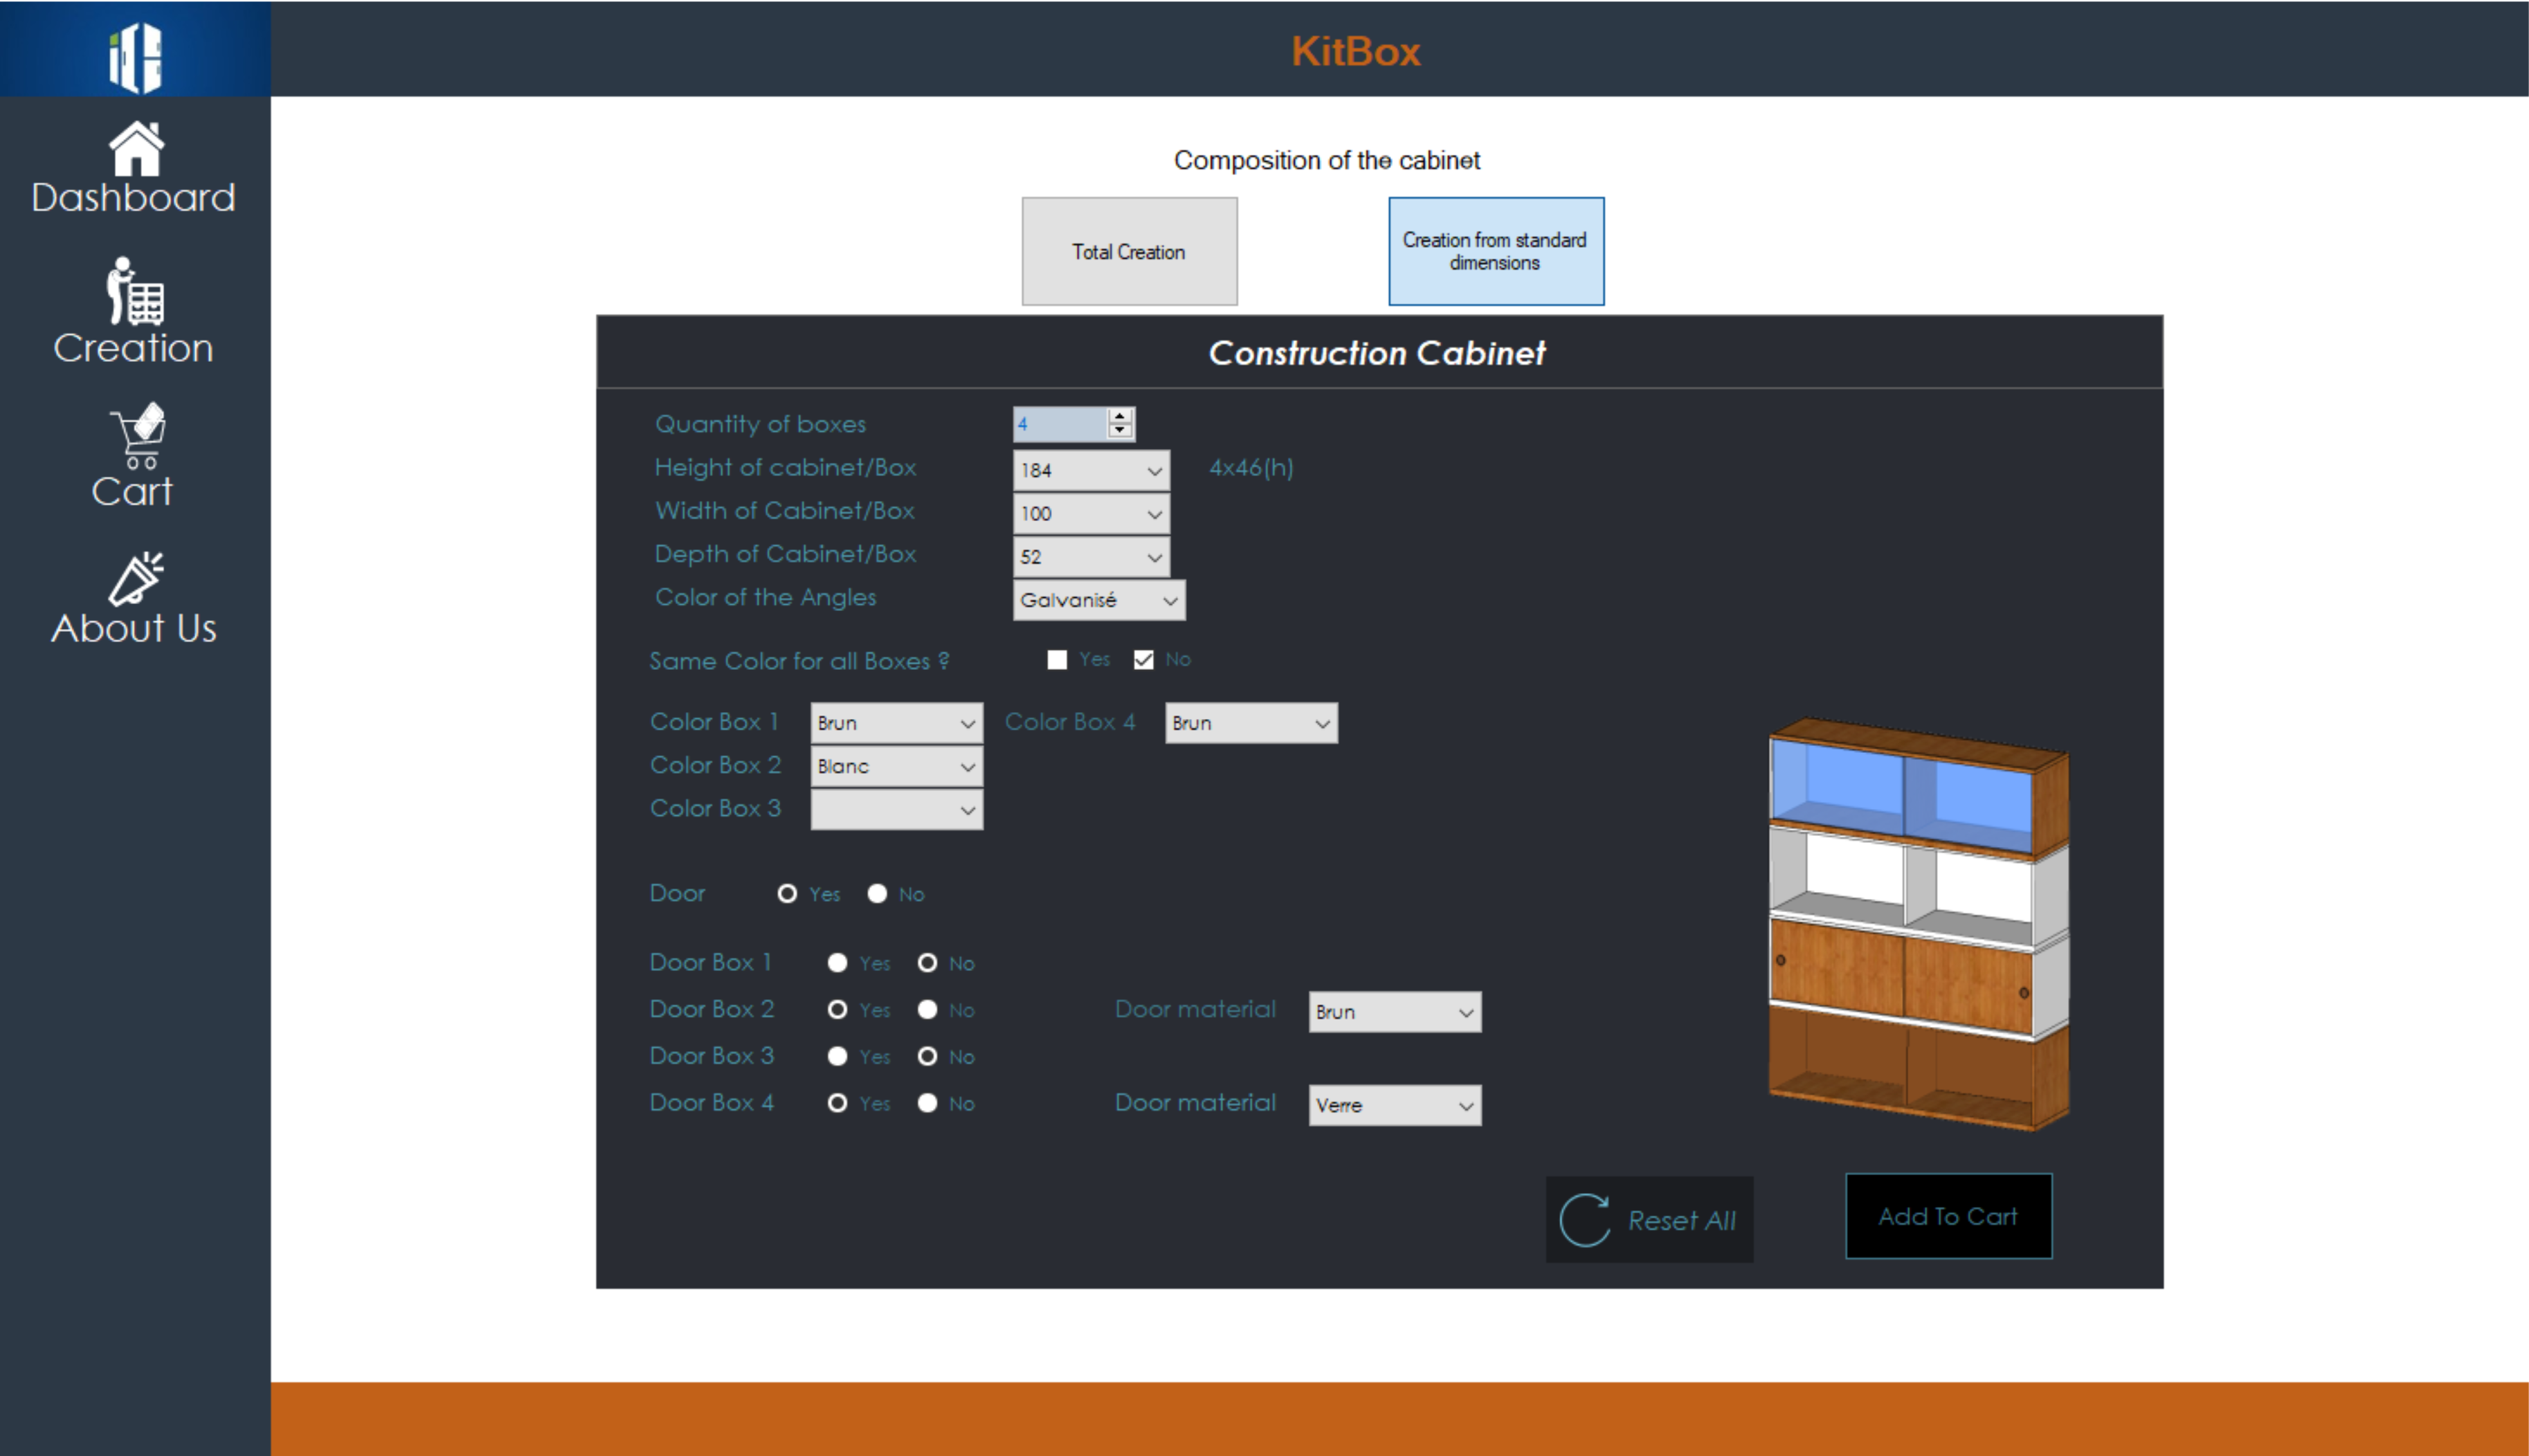
\includegraphics[height=110truemm,angle = 90]{Figures/CreationStandardFilled.PNG}
    		\rule{35em}{0.5pt}
    		\caption{Creation from standard dimensions after filling all features}
    		\label{standardtabfilled}
    	\end{figure*}
    	\vfill
	
	\newpage
	\subsection{Cart page}
    	\vfill
        \begin{figure*}[h!]
            \centering
    		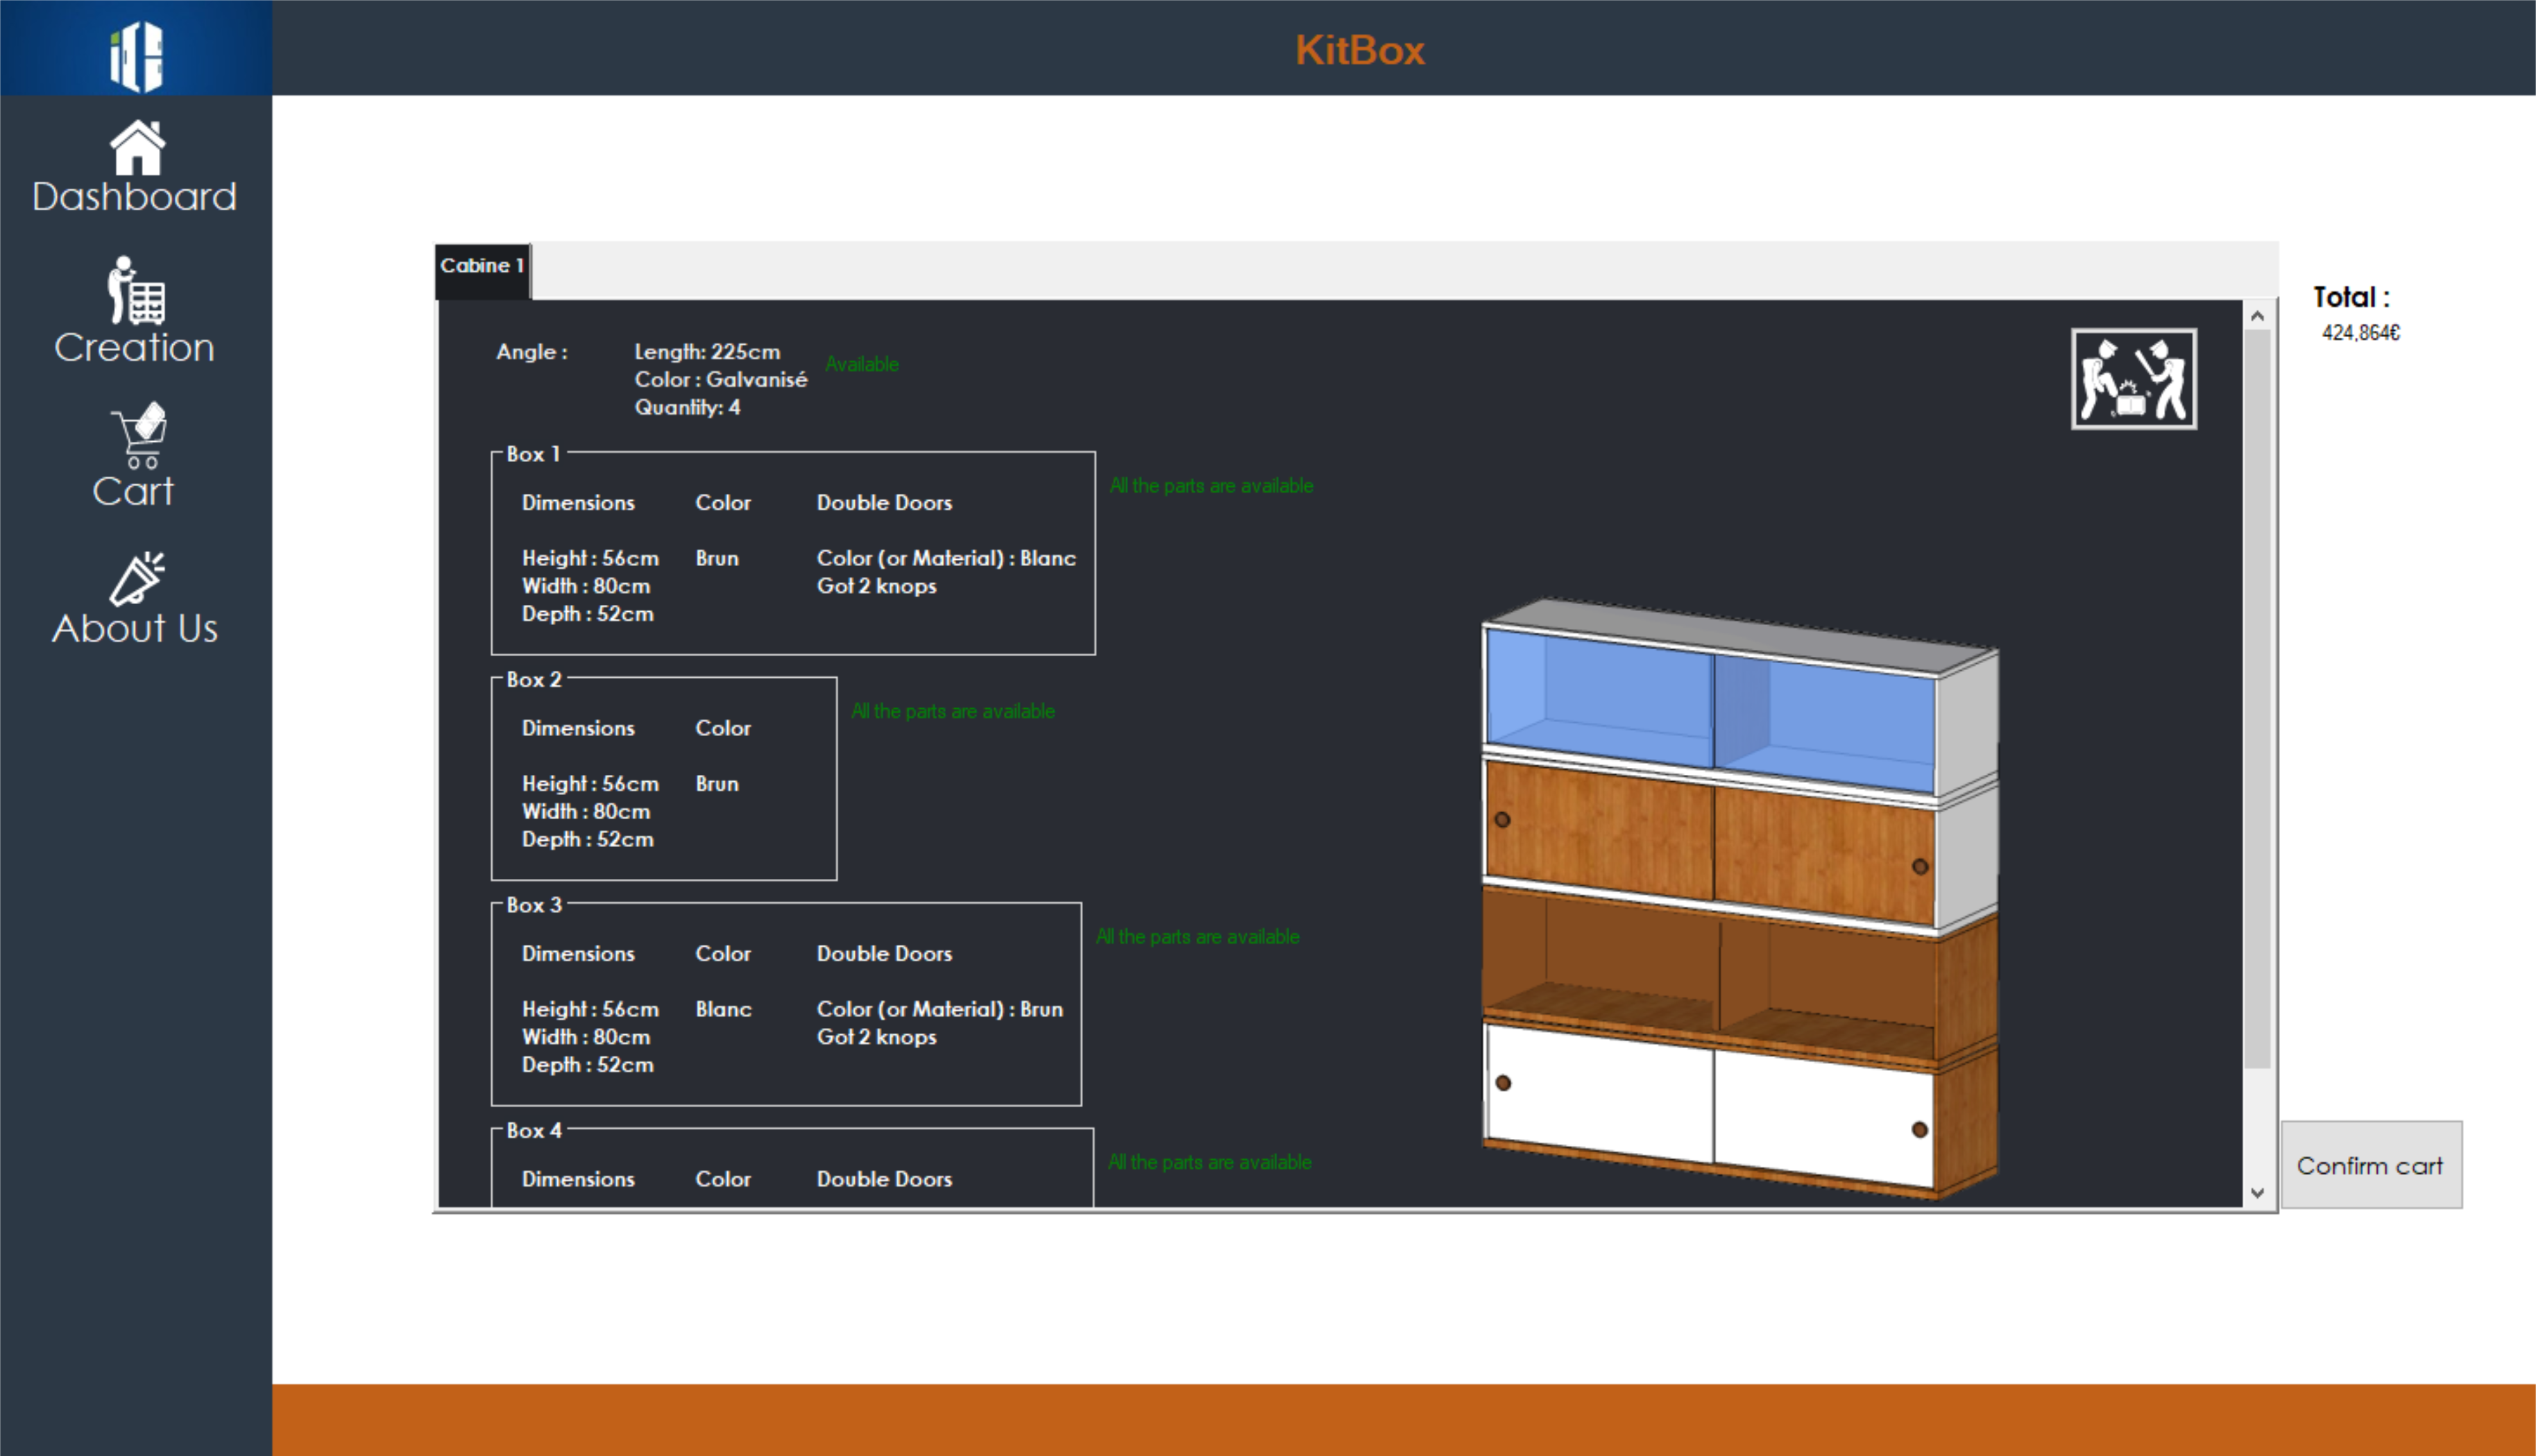
\includegraphics[width =1.2\textwidth,angle = 90]{Figures/CartPage.PNG}
    		\rule{35em}{0.5pt}
    		\caption{Cart page containing one four floors cabinet}
    		\label{carttab}
    	\end{figure*}
    	\vfill
    	
    \newpage
	\subsection{Cart page with mail}
    	\vfill
        \begin{figure*}[h!]
            \centering
    		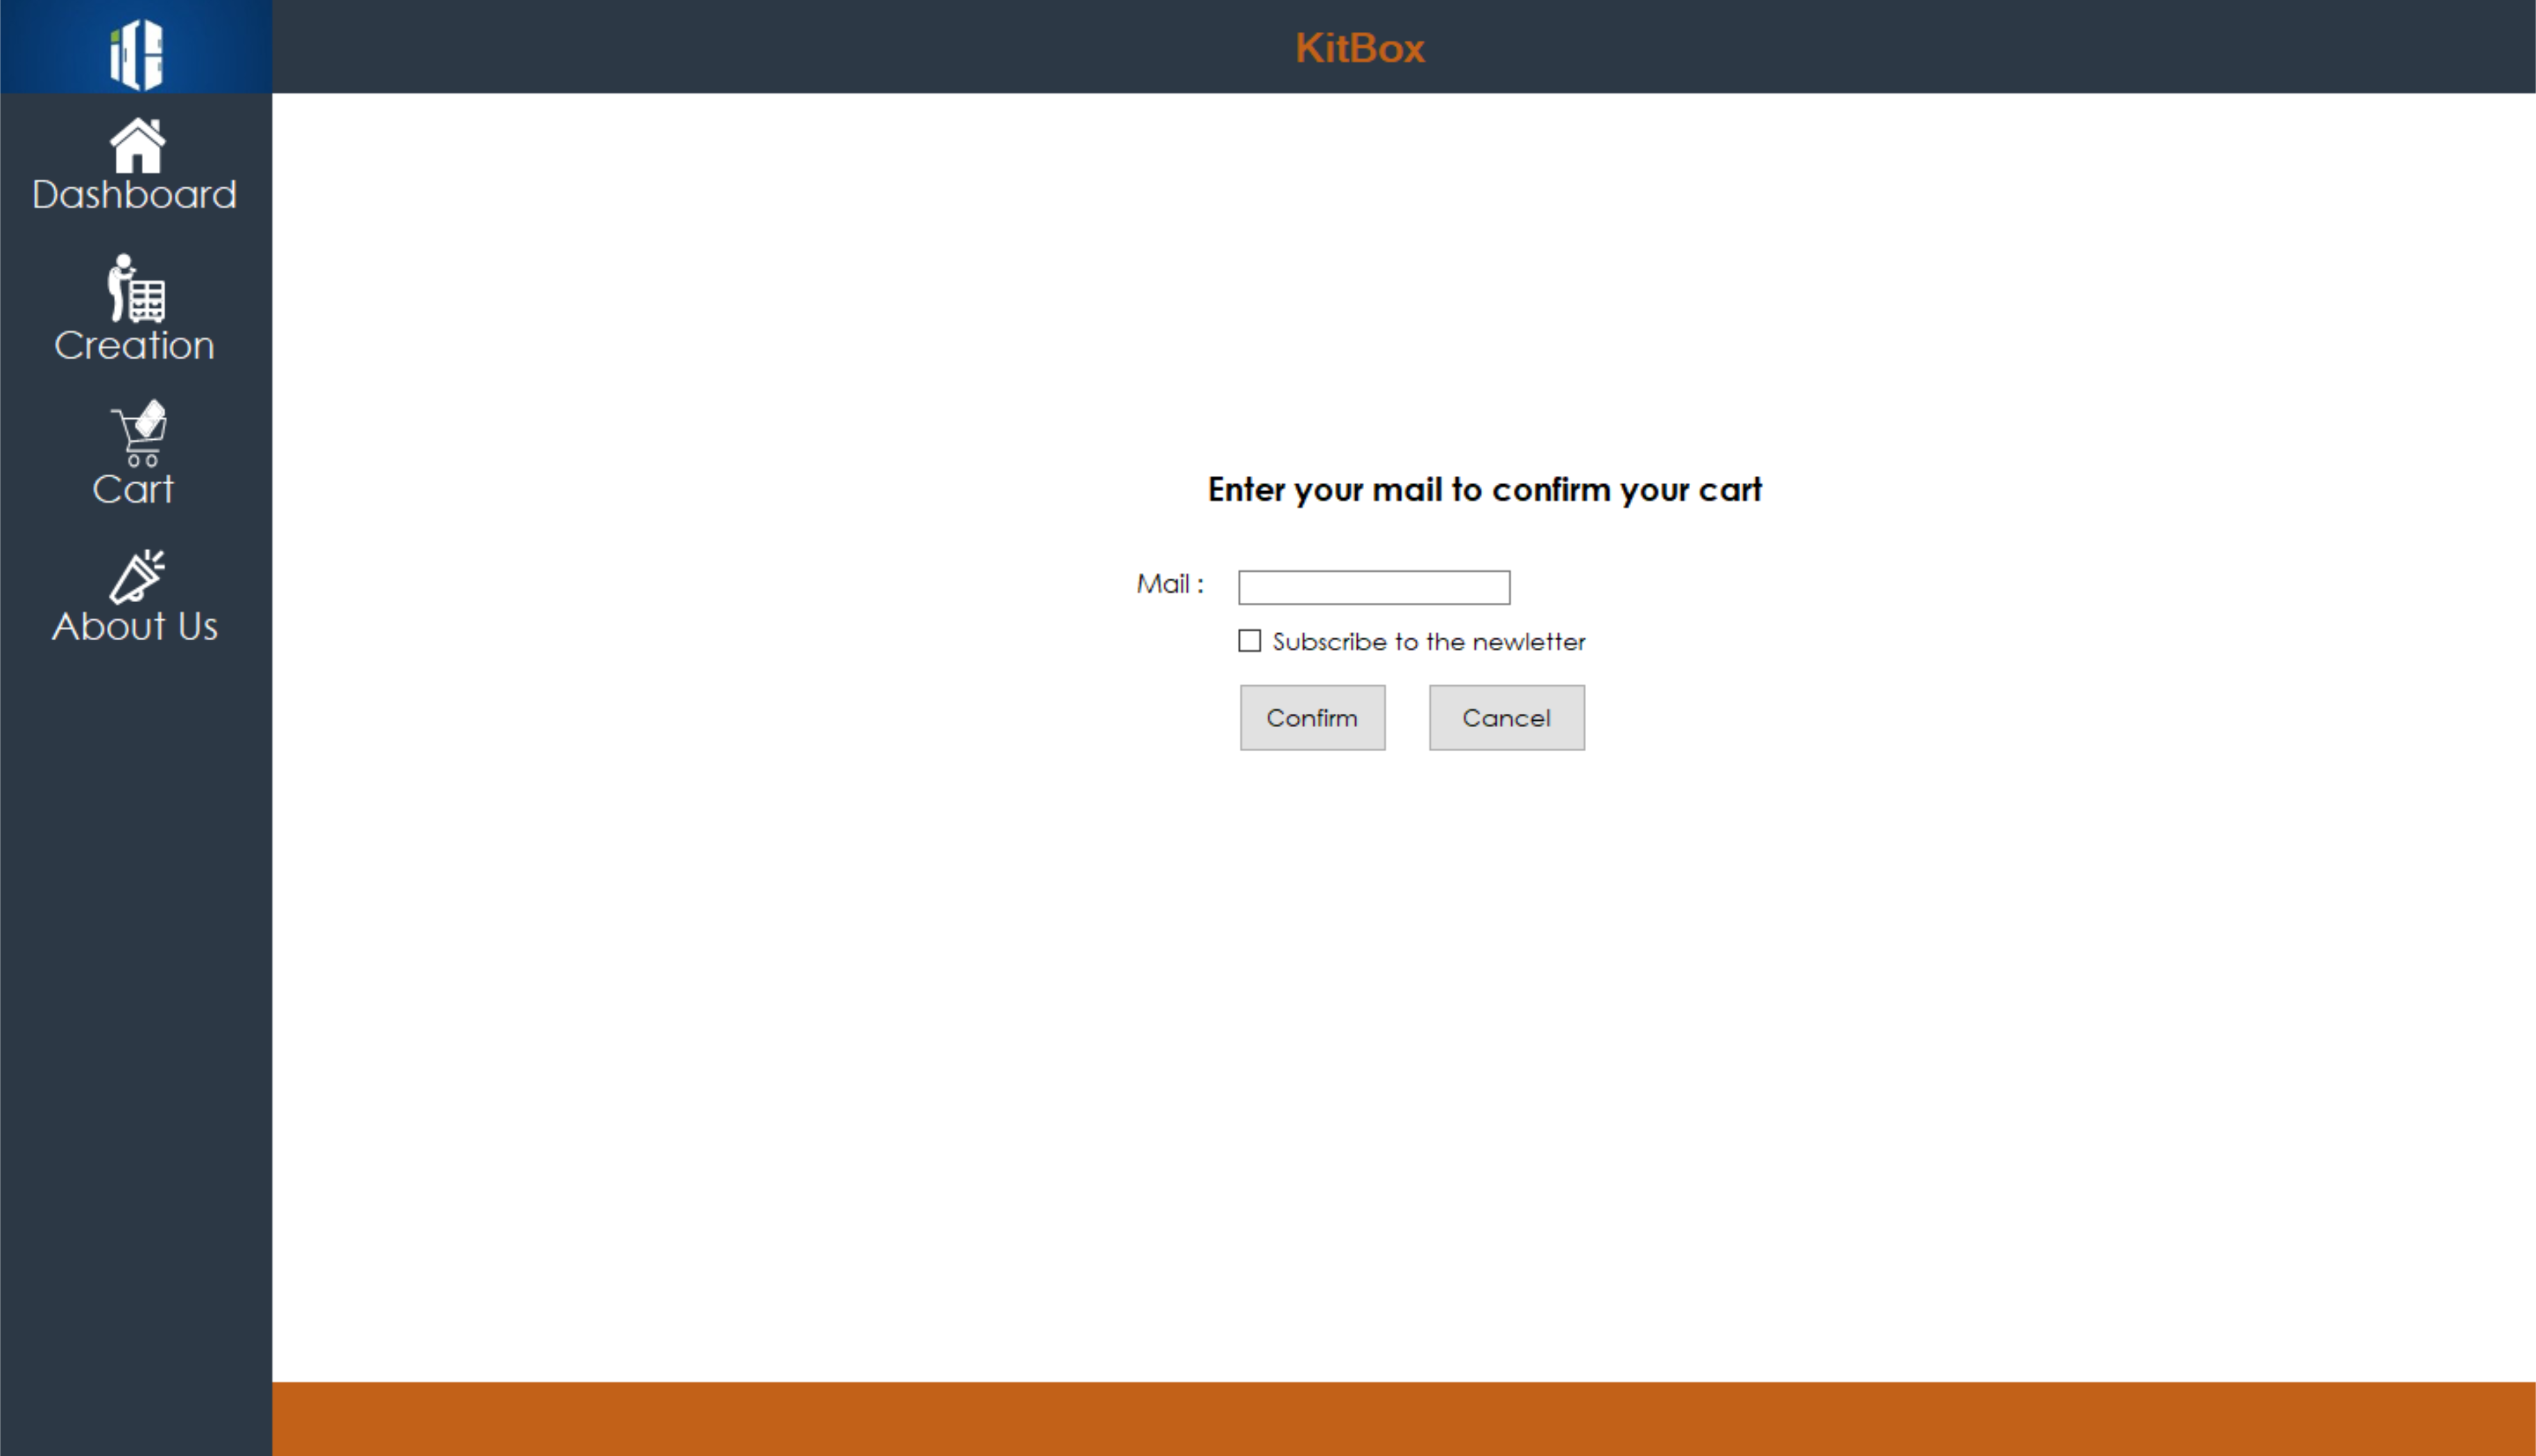
\includegraphics[width =1.2\textwidth,angle = 90]{Figures/CartPageMail.PNG}
    		\rule{35em}{0.5pt}
    		\caption{Client credentials to order cabinet}
    		\label{authtab}
    	\end{figure*}
    	\vfill
    	
    \newpage
	\subsection{About Us page}
    	\vfill
        \begin{figure*}[h!]
            \centering
    		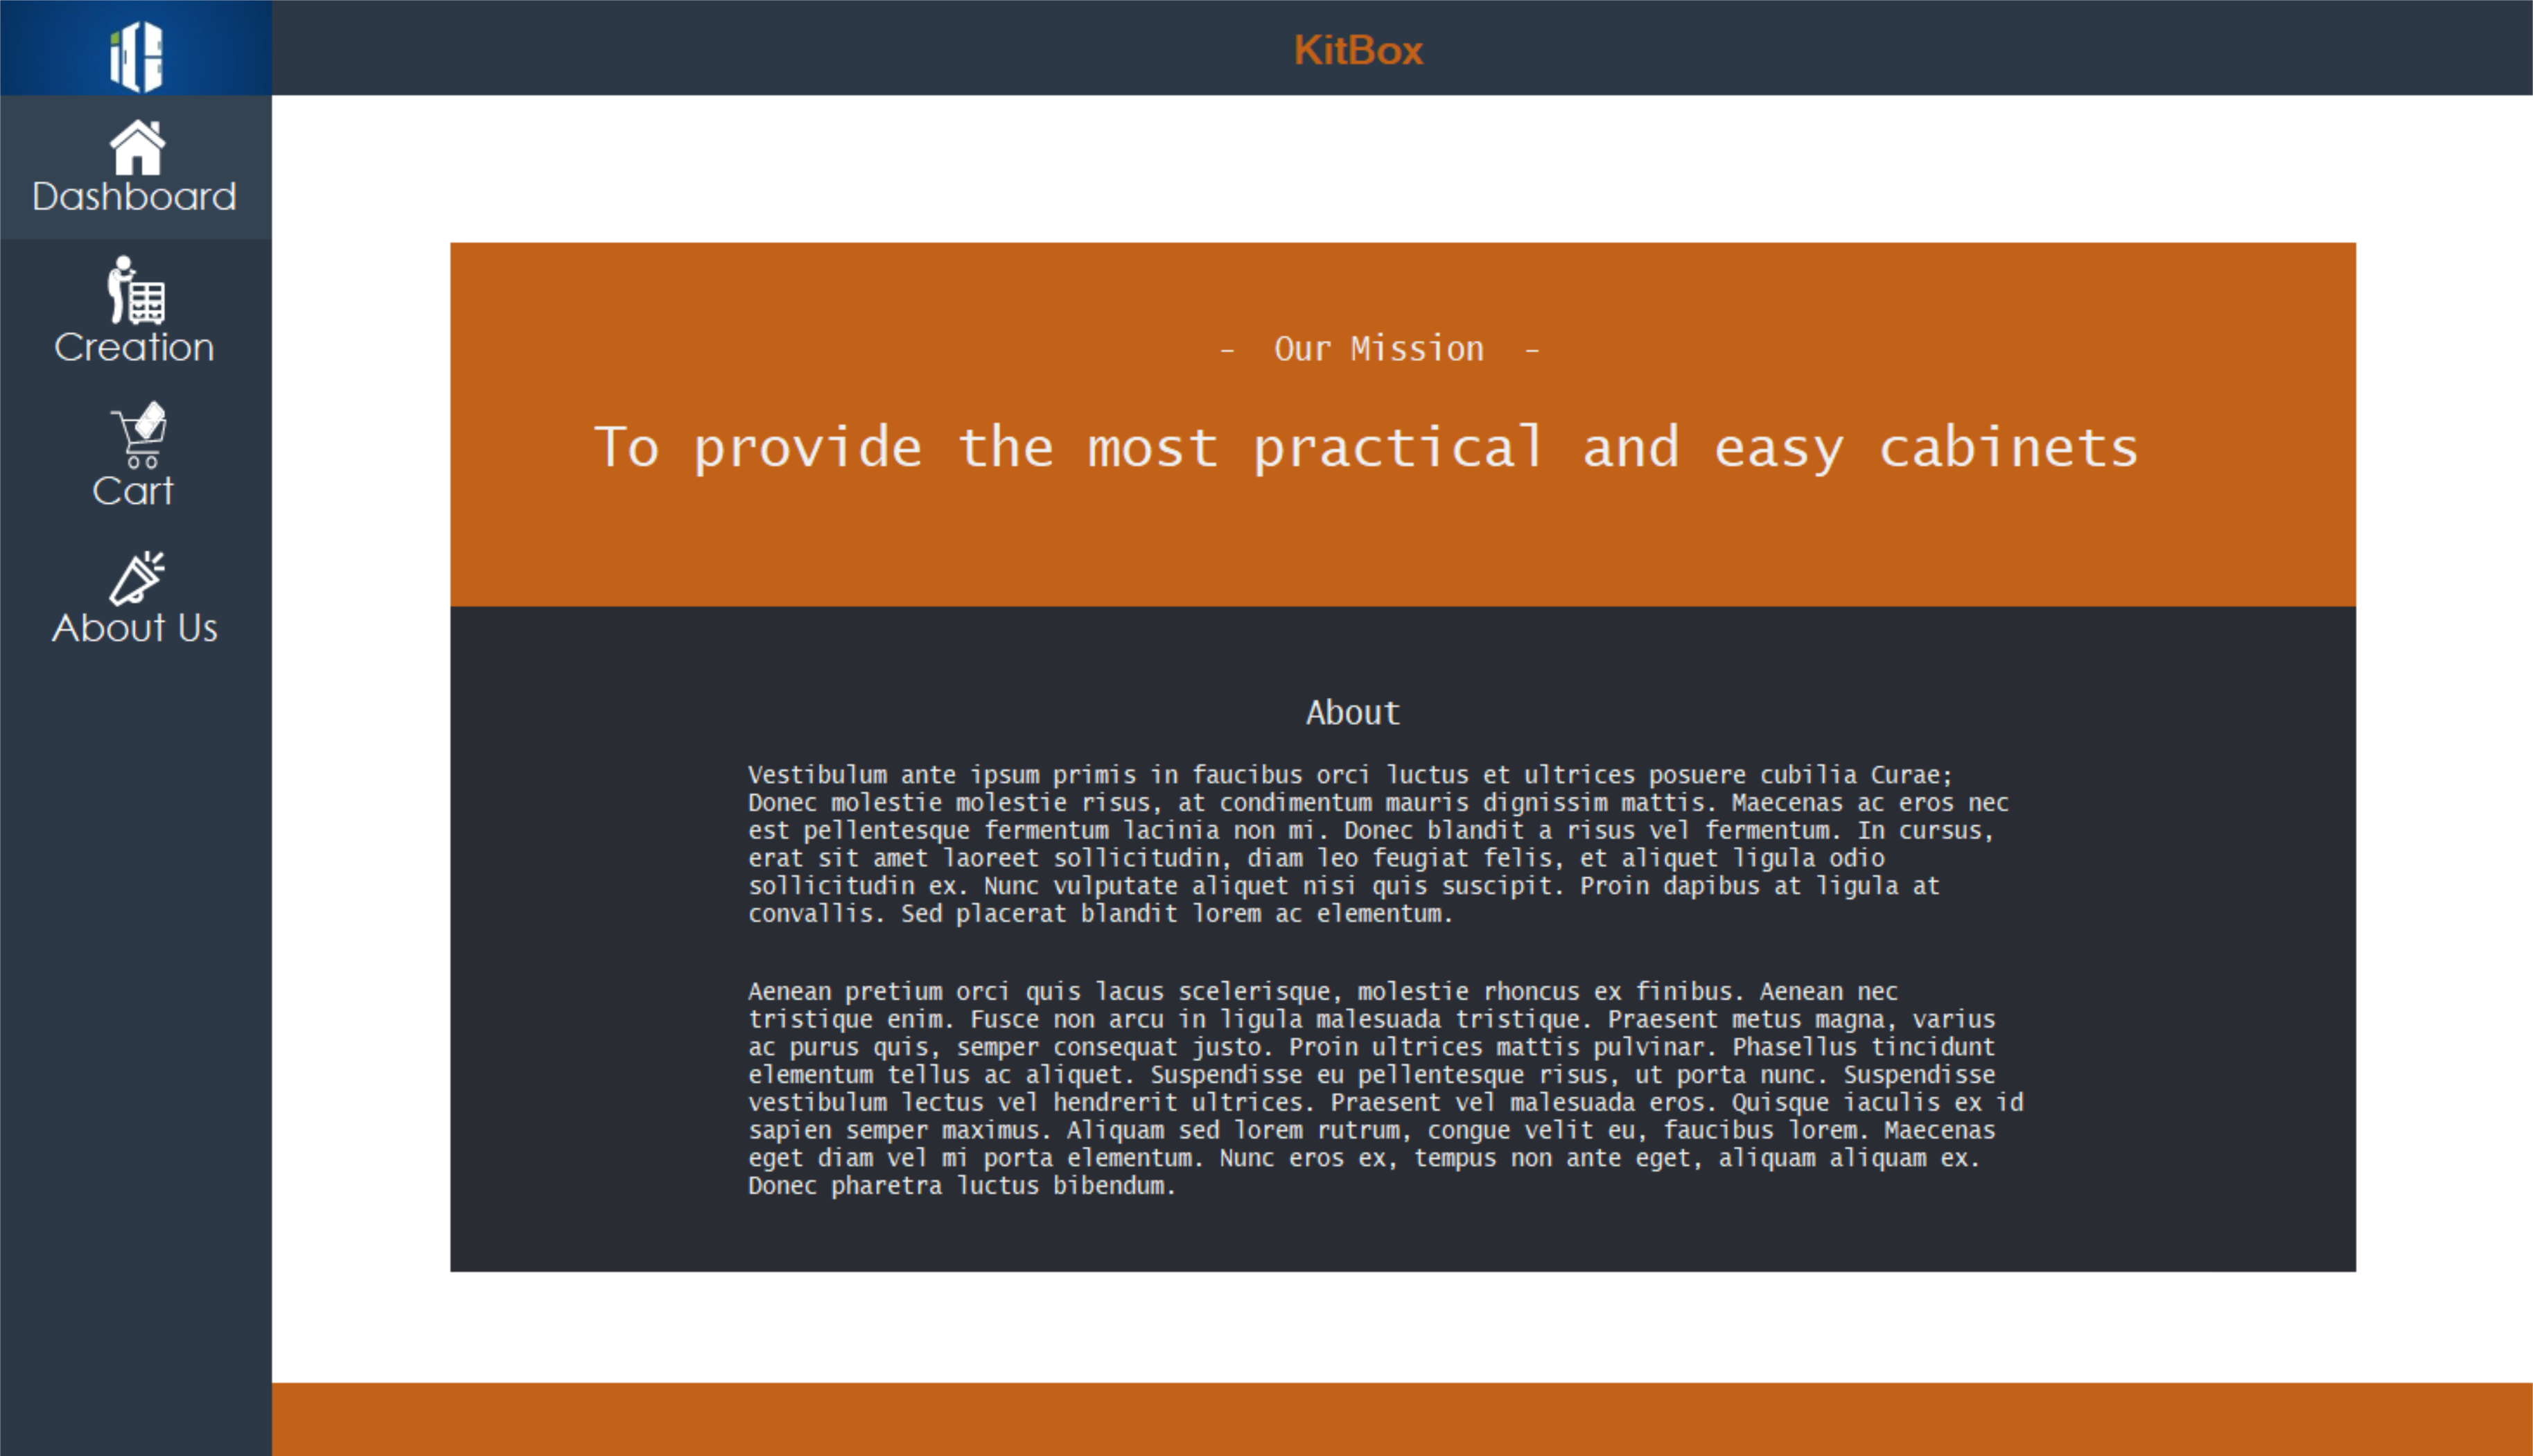
\includegraphics[width =1.2\textwidth,angle = 90]{Figures/AboutUs.PNG}
    		\rule{35em}{0.5pt}
    		\caption{About Us page}
    		\label{aboutus}
    	\end{figure*}
    	\vfill

\newpage
\section{Storekeeper Interface}
\label{Storekeeperinterface}
    \subsection{Stock Manager Tab Interface}
        \vfill
        \begin{figure*}[h!]
            \centering
    		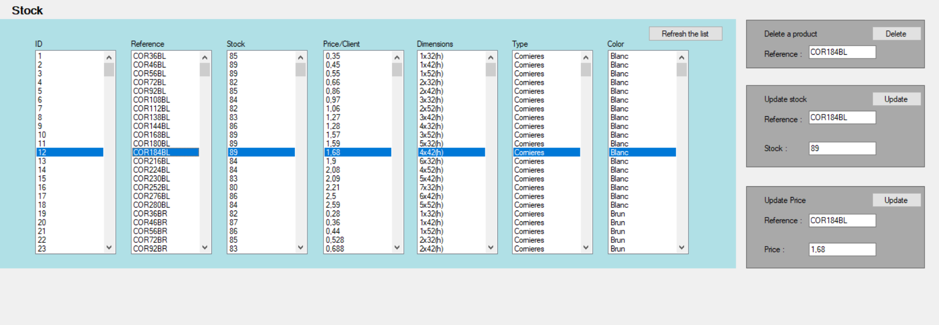
\includegraphics[width =1.2\textwidth,angle = 90]{Figures/StockManagerTab.png}
    		\rule{35em}{0.5pt}
    		\caption{Stock Manager Interface}
    		\label{stocktab}
    	\end{figure*}
    	\vfill
    	
	\newpage
	\subsection{New Product or Supplier Tab Interface}
    	\vfill
        \begin{figure*}[h!]
            \centering
    		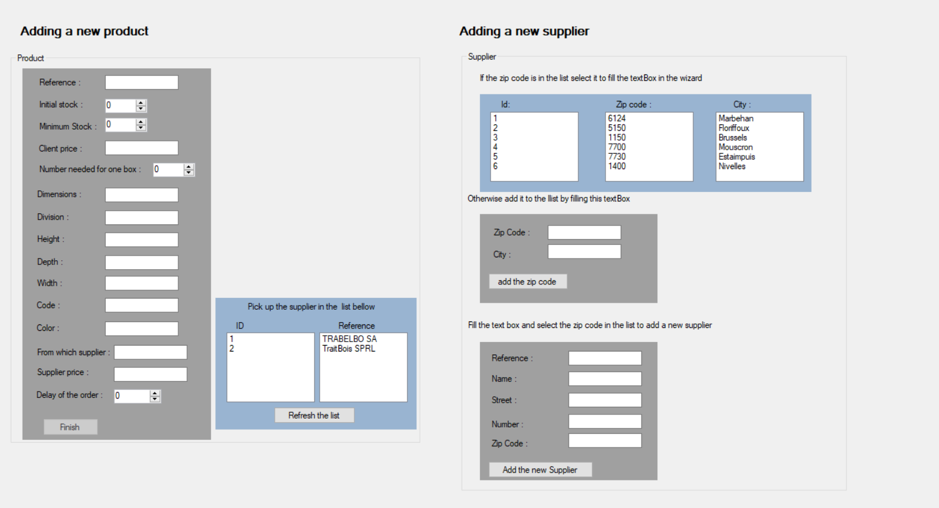
\includegraphics[width =1.2\textwidth,angle = 90]{Figures/SupplierTab.png}
    		\rule{35em}{0.5pt}
    		\caption{New Product and Supplier Interface}
    		\label{suppliertab}
    	\end{figure*}
    	\vfill
    	
	\newpage
	\subsection{Order Tab Interface}
    	\vfill
        \begin{figure*}[h!]
            \centering
    		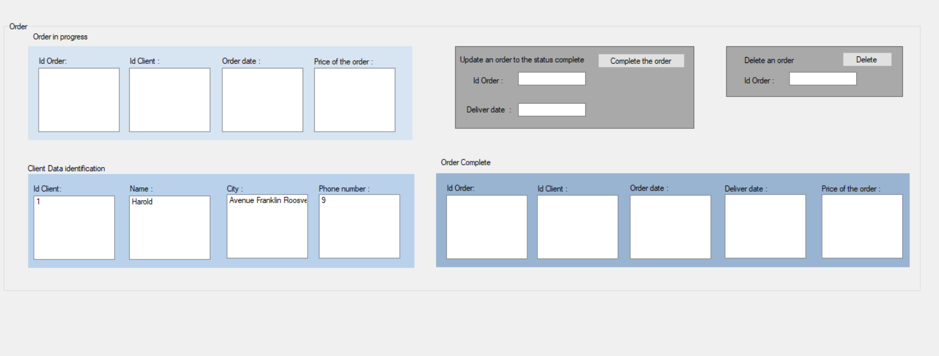
\includegraphics[width =1.2\textwidth,angle = 90]{Figures/OrderTab.png}
    		\rule{35em}{0.5pt}
    		\caption{Order Interface}
    		\label{ordermanagertab}
    	\end{figure*}
    	\vfill
    	
	\newpage
	\subsection{Client Tab Interface}
    	\vfill
        \begin{figure*}[h!]
            \centering
    		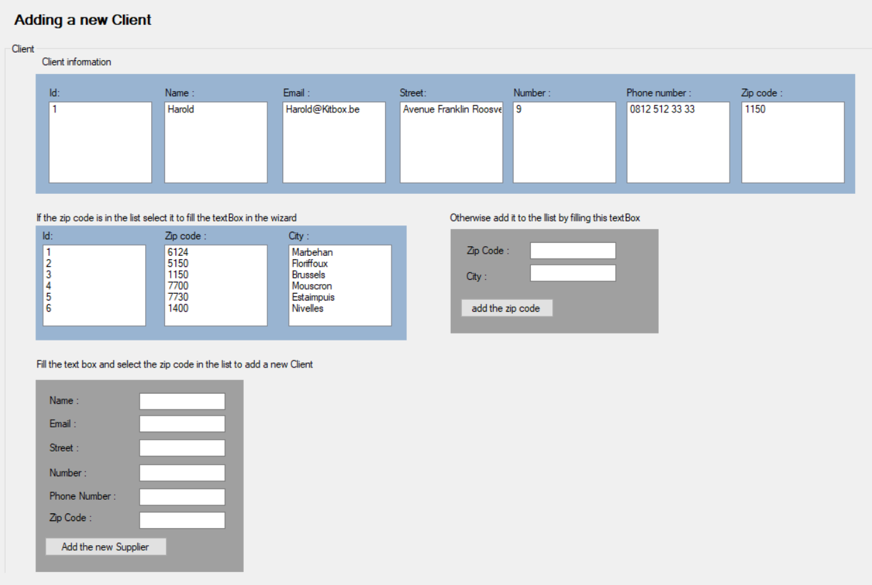
\includegraphics[width =1.2\textwidth,angle = 90]{Figures/ClientTab.png}
    		\rule{35em}{0.5pt}
    		\caption{Interface where you can find the customer's information}
    		\label{clientmanagertab}
    	\end{figure*}
    	\vfill
\end{document}
